\clearpage

\section{Validation of the $\bar{\nu}/\nu$ joint analysis}
\label{sec:validation}

The validation of the fit is performed first by comparing the confidence intervals, obtained
with Asimov data sets corresponding to the oscillation parameters in \cref{tab:osc_params_joint_asimov}
%as well as the Run 1-4 data, 
with the other group analyses \cite{Mach3JointFitRun16}.
Then the coverage study is performed for 1-dimensional $\delta_{CP}$ with reactor constraint fits,
in order to verify if the ``constant $\Delta \chi^2$" method is reliable or
the ``Feldman-Cousins" method is needed.
%Pull studies will be shown for 1-dimensional fits of the following oscillation parameters:
%$\delta_{CP}$, $\sin^2 \theta_{13}$, $\sin^2 \theta_{23}$ and $|\Delta m^2_{32}|$,
%for which $\pm 1 \sigma$ ranges will be quoted by using the ``constant $\Delta \chi^2$ method".
%Since the nuisance parameters are marginalised in the fit, pull studies for these parameters do not make sense
%and will not be shown.


%
% Sensitivities and comparisons with other analysis groups
%

\subsection{Sensitivity studies}
\label{sec:sensi}

The critical values of constant $\Delta \chi^2$ method
in 1-dimensional confidence intervals are given 
by $Z\sigma = \sqrt{\Delta \chi^2}$  
where $Z$ is the number of standard deviations that
defines the confidence level.
For 90\% CL the critical value is 2.71.
The critical values for 2-dimensional fits are 2.3 and 4.61
respectively for 68\% and 90\% CL.
A detailed table with the critical values for 1- and 2-dimensional confidence
intervals can be found in \cite{pdg_stat}.

In \cref{fig:validation_sensi_dcp} the sensitivity to $\delta_{CP}$ 
with reactor constraint and T2K only is shown for the Asimov data sets A and B.
%and compared with the result obtained by the other analysis groups.

\begin{figure*}[htb]
\center
%
\includegraphics[width=0.9\textwidth]{./images/missing_plot-eps-converted-to.pdf}
%
\includegraphics[width=0.9\textwidth]{./images/missing_plot-eps-converted-to.pdf}
\begin{subfigure}[b]{0.49\textwidth}
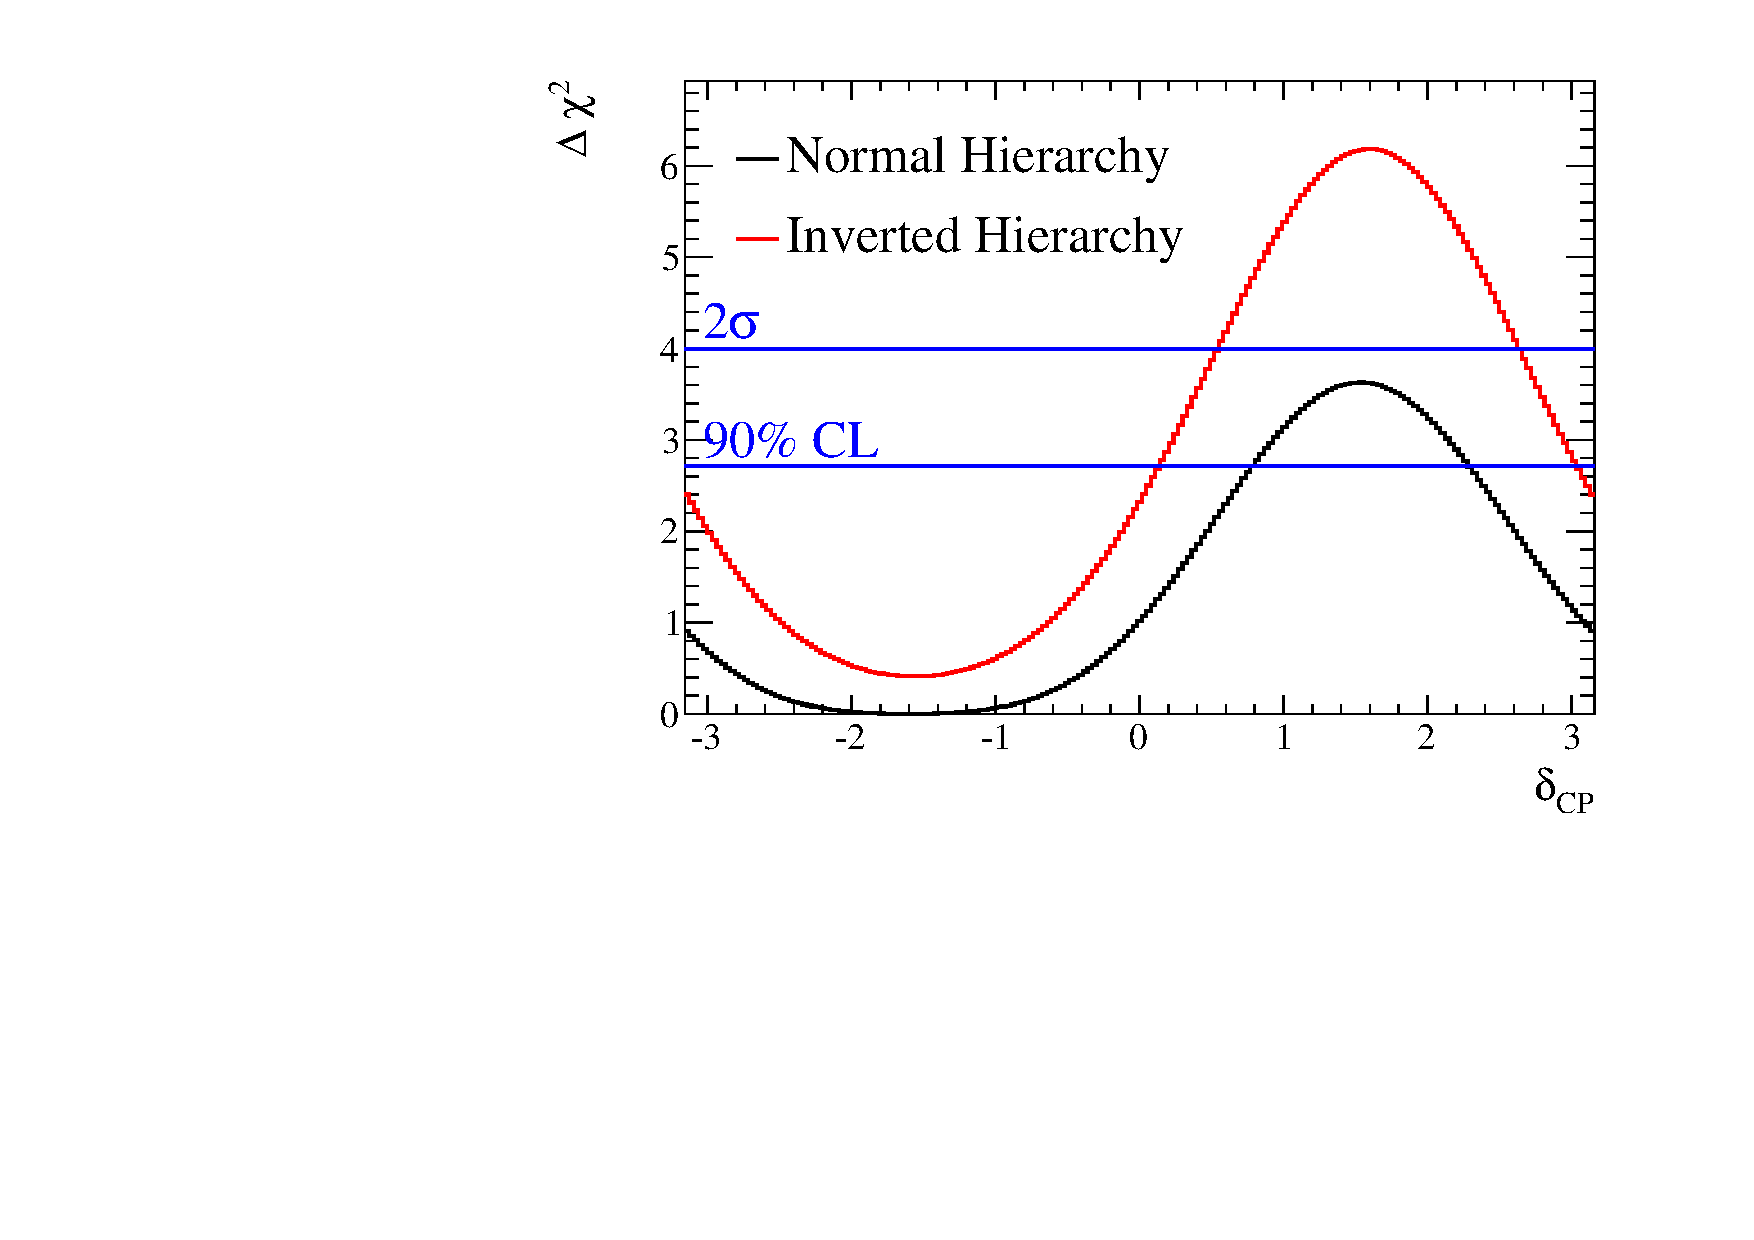
\includegraphics[width=0.9\textwidth]{./joint_plots/sensitivities/dcp_1D/dcp_react_Asimov_A.pdf}
\caption{Asimov A: with reactor constraint}
\end{subfigure}
\begin{subfigure}[b]{0.49\textwidth}
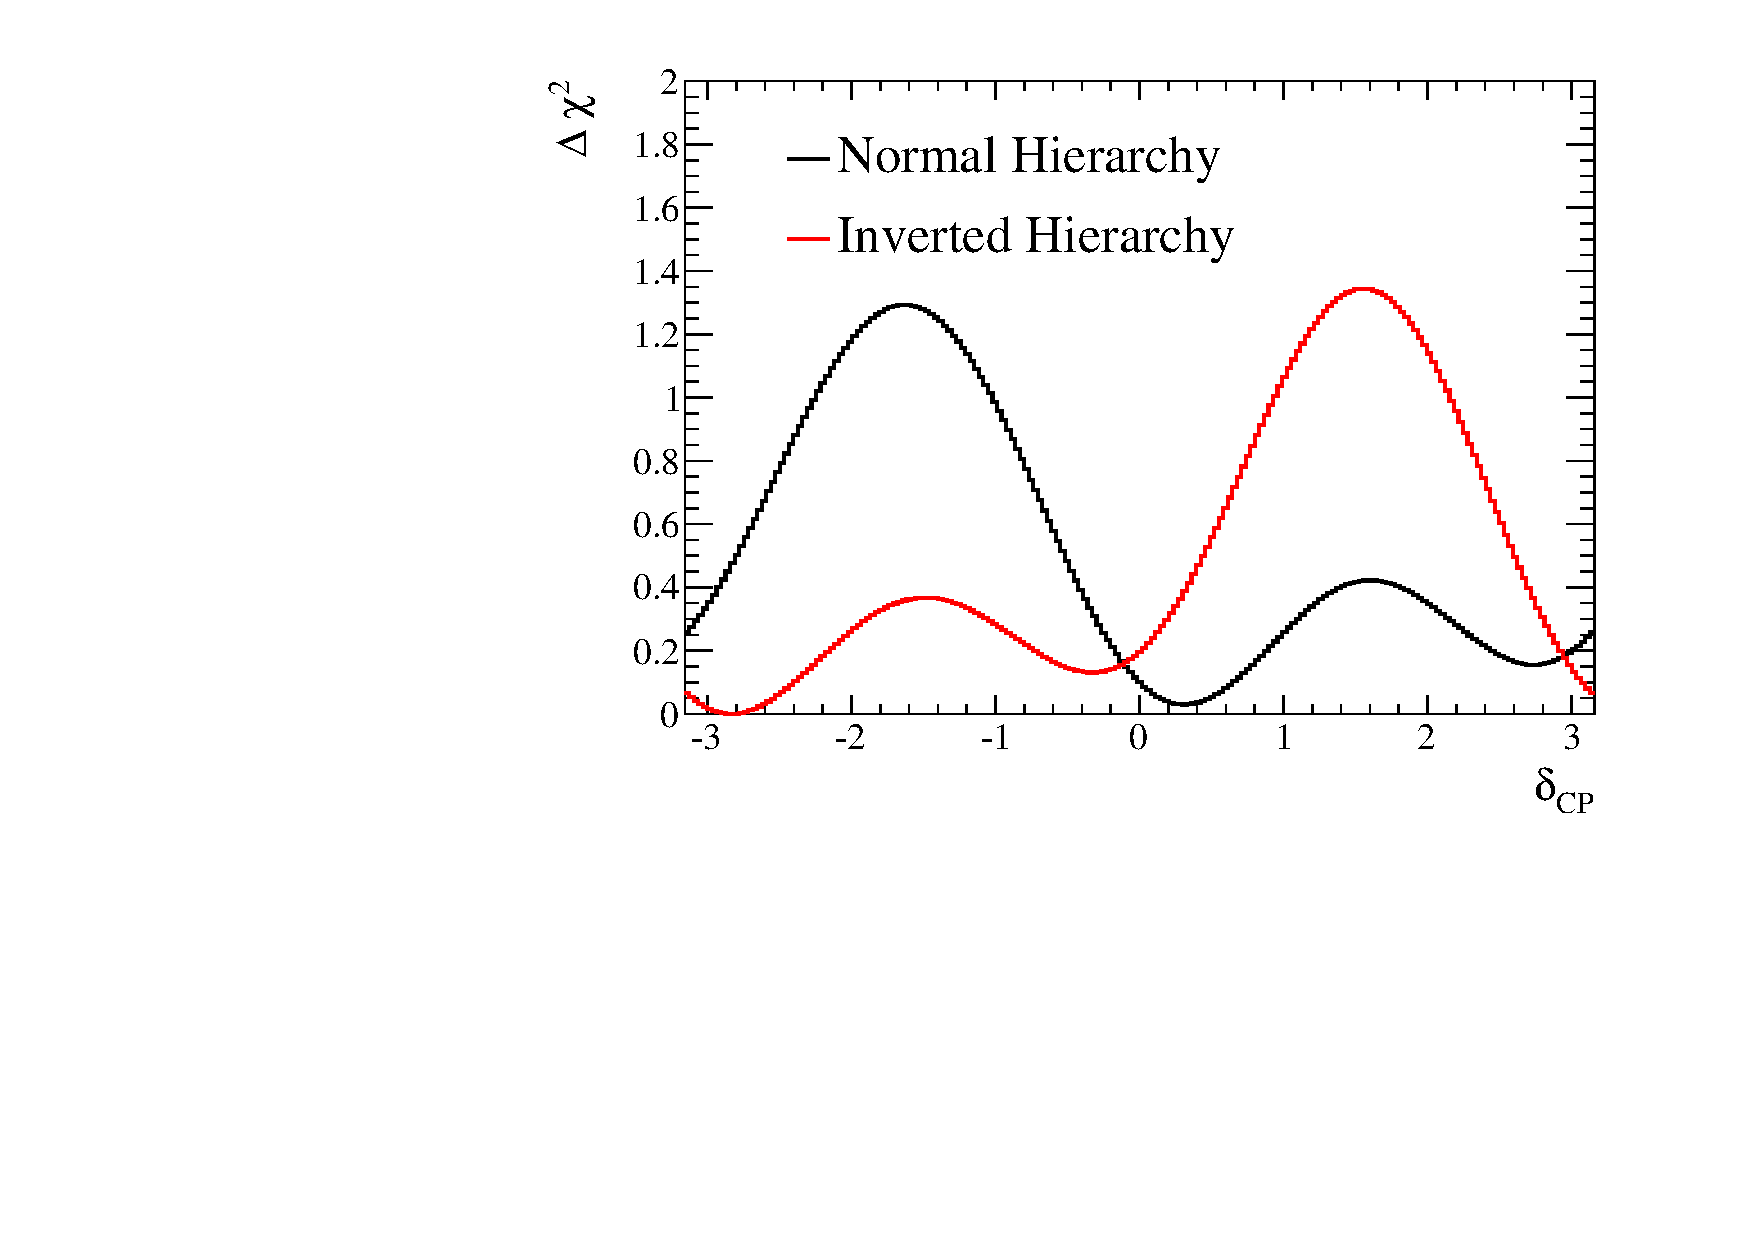
\includegraphics[width=0.9\textwidth]{./joint_plots/sensitivities/dcp_1D/dcp_react_Asimov_B.pdf} 
\caption{Asimov B: with reactor constraint}
\end{subfigure}
\begin{subfigure}[b]{0.49\textwidth}
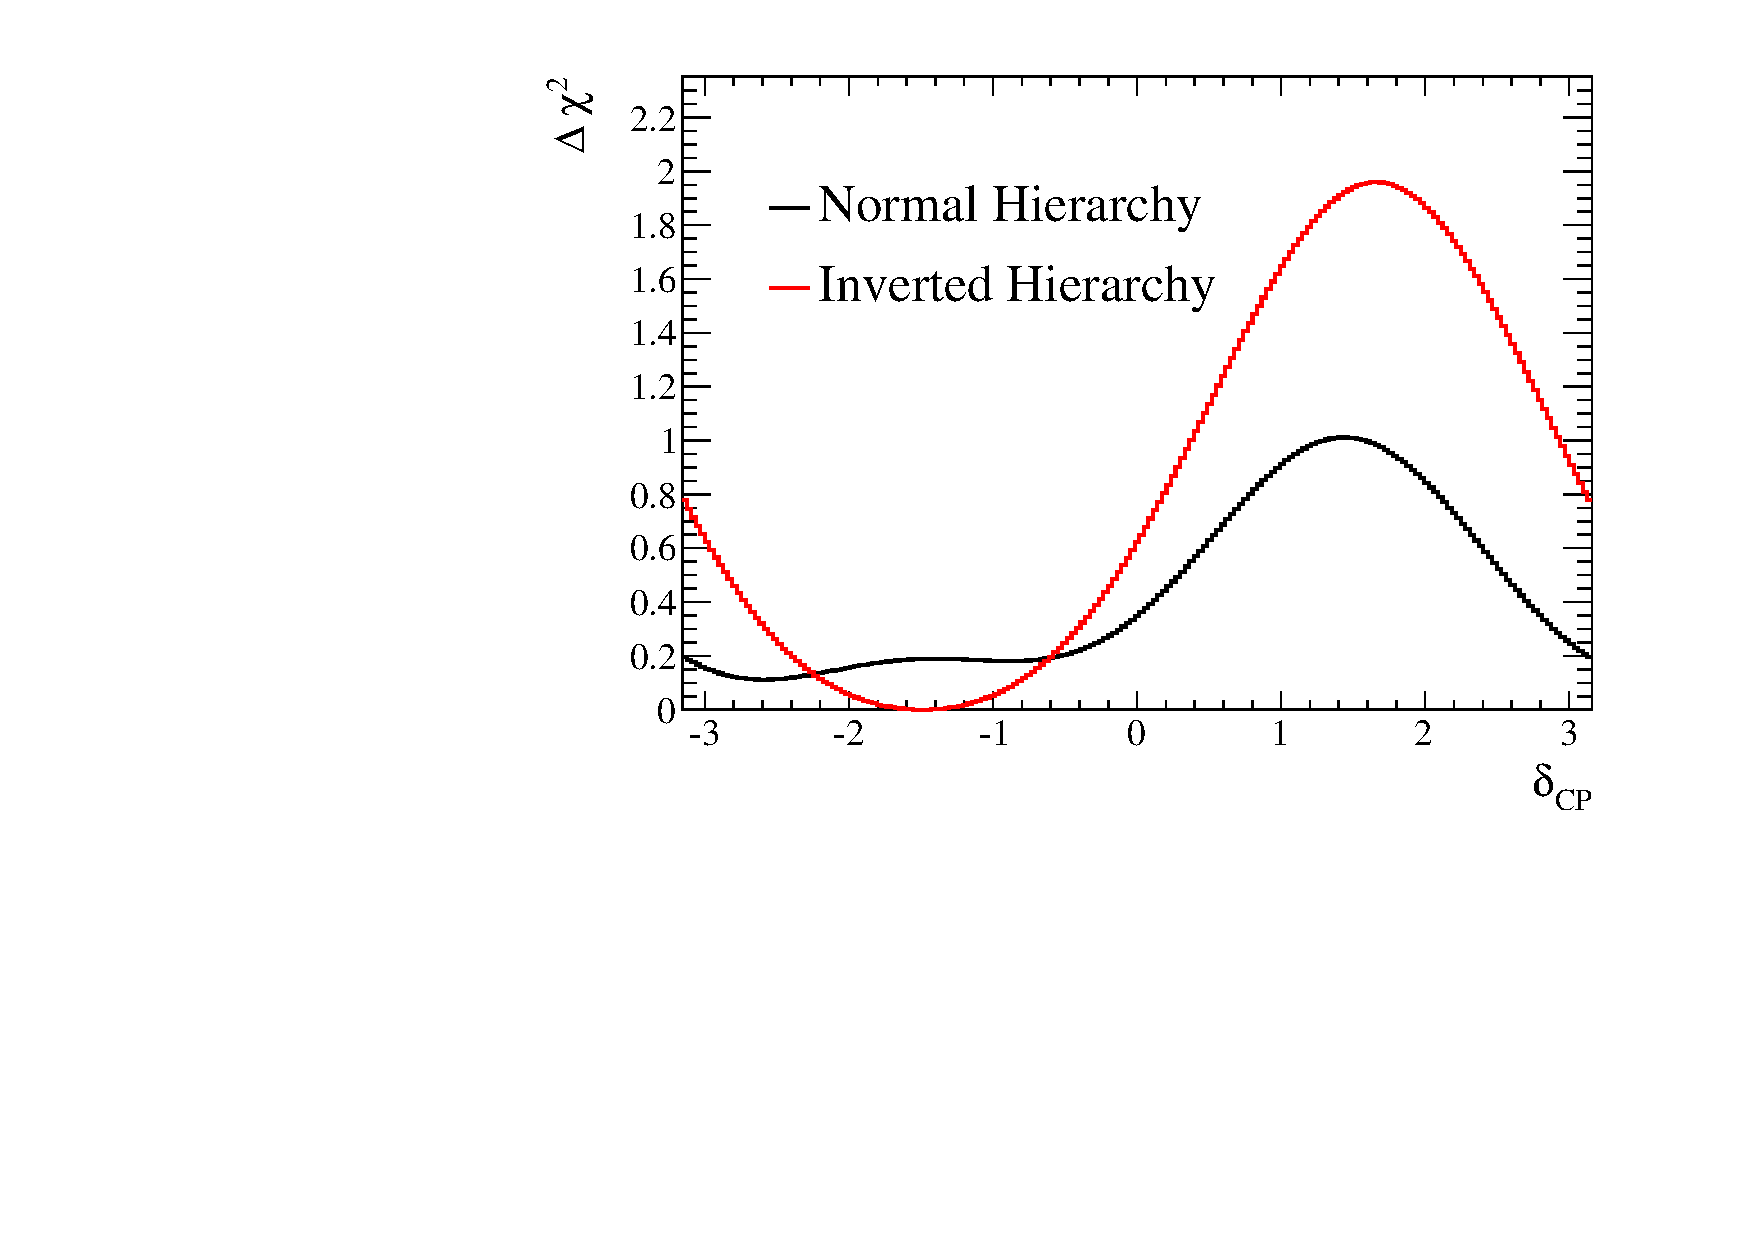
\includegraphics[width=0.9\textwidth]{./joint_plots/sensitivities/dcp_1D/dcp_t2konly_Asimov_A.pdf}
\caption{Asimov A: with T2K only}
\end{subfigure}
\begin{subfigure}[b]{0.49\textwidth}
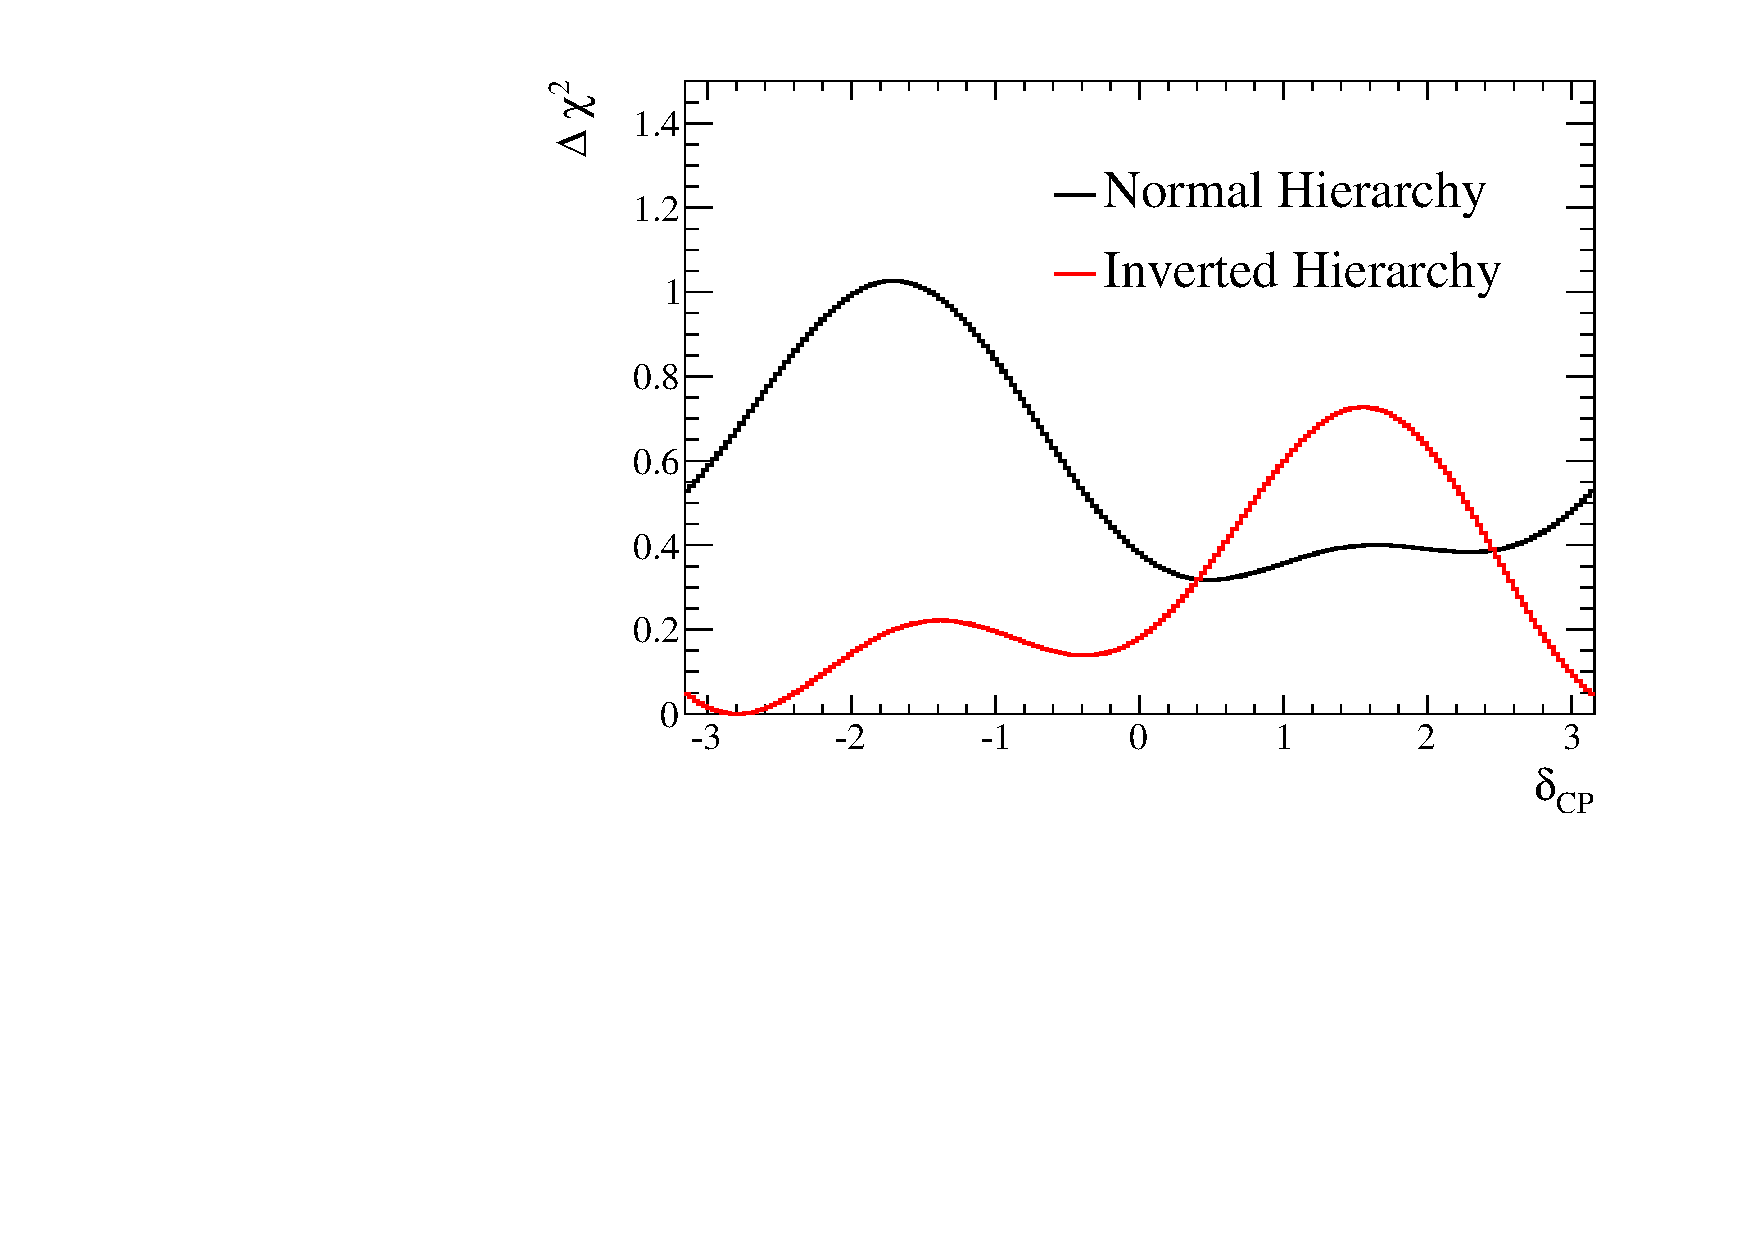
\includegraphics[width=0.9\textwidth]{./joint_plots/sensitivities/dcp_1D/dcp_t2konly_Asimov_B.pdf}
\caption{Asimov B: with T2K only}
\end{subfigure}
\caption {
%{\large{SENSI DELTACHISQ 1D DELTACP W/ AND W/O REACTORS}}
The expected $\Delta \chi^2$ distribution as a function of $\delta_{CP}$ 
for the Asimov data sets A and B of \cref{tab:osc_params_joint_asimov} 
corresponding to the Run 1-6 statistics is shown.
The mass hierarchy is minimized:
both the normal and inverted hierarchy $\chi^2$ distributions 
are shifted to the same global best-fit $\chi^2$ value,
which is taken as the minimum between normal and inverted hierarchy.
}
\label{fig:validation_sensi_dcp}
\end{figure*}

%The sensitivity to $\sin^2 \theta_{13}$ Vs $\delta_{CP}$ 
%with reactor constraint and T2K only data,
%is shown in \cref{fig:validation_sensi_2d_reactors}, 
%while $\sin^2 \theta_{23}$ Vs $\Delta m^2_{32}$ ($\Delta m^2_{13}$) with reactor constraint 
%is shown in \cref{fig:validation_sensi_2d_t2konly}.
%In both cases the normal and inverted hierarchy contours are set independently,
%i.e. each calculated with respect to its own minimum $\chi^2$ value
%and not the global minimum as a function of the mass hierarchy.

\Cref{fig:validation_sensi_2d_reactors} shows the sensitivity to 
$\sin^2 \theta_{13}$ Vs $\delta_{CP}$  and $\sin^2 \theta_{23}$ Vs $\Delta m^2_{32}$ ($\Delta m^2_{13}$) 
with the reactor constraint. 
\Cref{fig:validation_sensi_2d_t2konly}
shows the sensitivity to $\sin^2 \theta_{13}$ Vs $\delta_{CP}$  with T2K data only. 
In both \cref{fig:validation_sensi_2d_reactors} and~\ref{fig:validation_sensi_2d_t2konly}, 
normal and inverted hierarchy contours are set independently, 
i.e. each calculated with respect to its own minimum $\chi^2$ value
and not the global minimum as a function of the mass hierarchy.

\begin{figure*}[htb]
\center
%
\includegraphics[width=0.9\textwidth]{./images/missing_plot-eps-converted-to.pdf}
%
\includegraphics[width=0.9\textwidth]{./images/missing_plot-eps-converted-to.pdf}
%
\includegraphics[width=0.9\textwidth]{./images/missing_plot-eps-converted-to.pdf}
%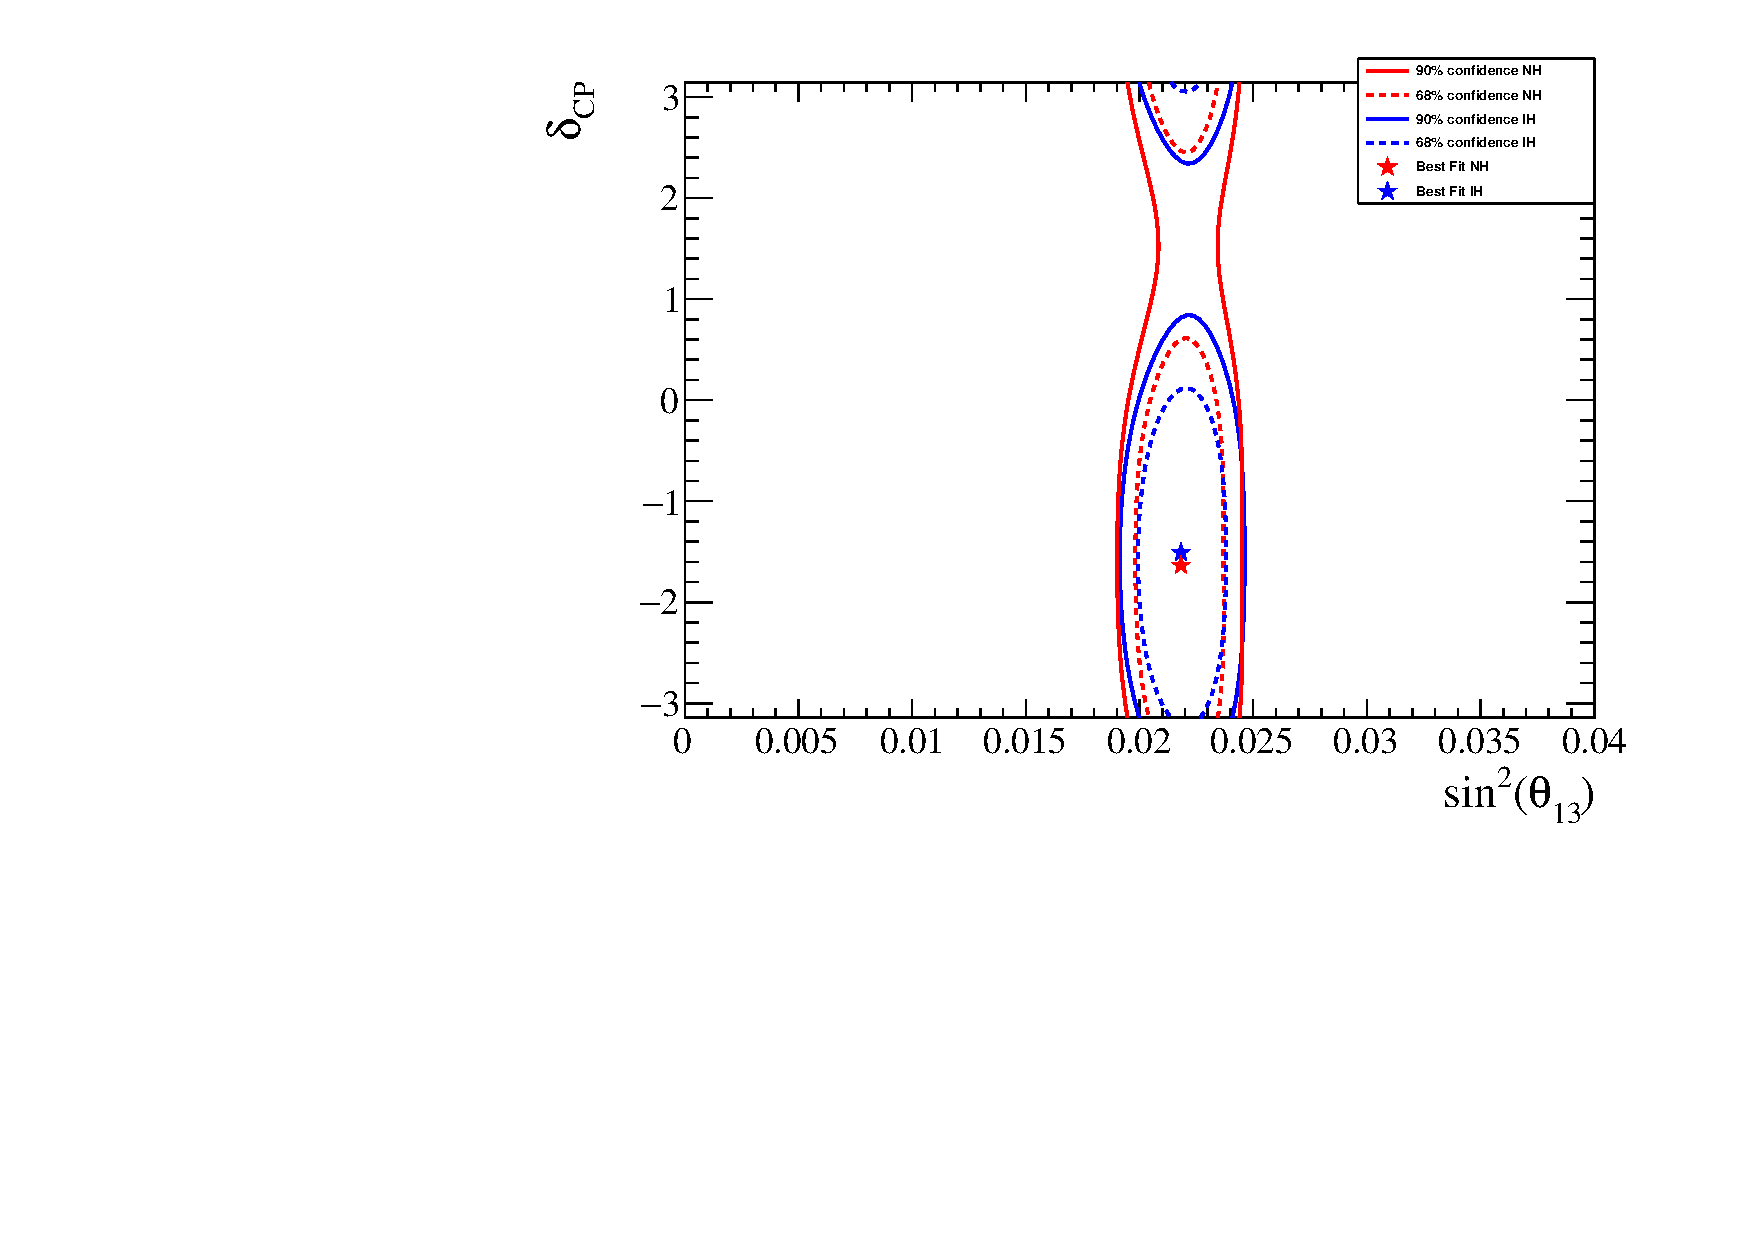
\includegraphics[width=0.9\textwidth]{./joint_plots/sensitivities/2D/cp13_reactor/cp13_reactor_A.pdf}
%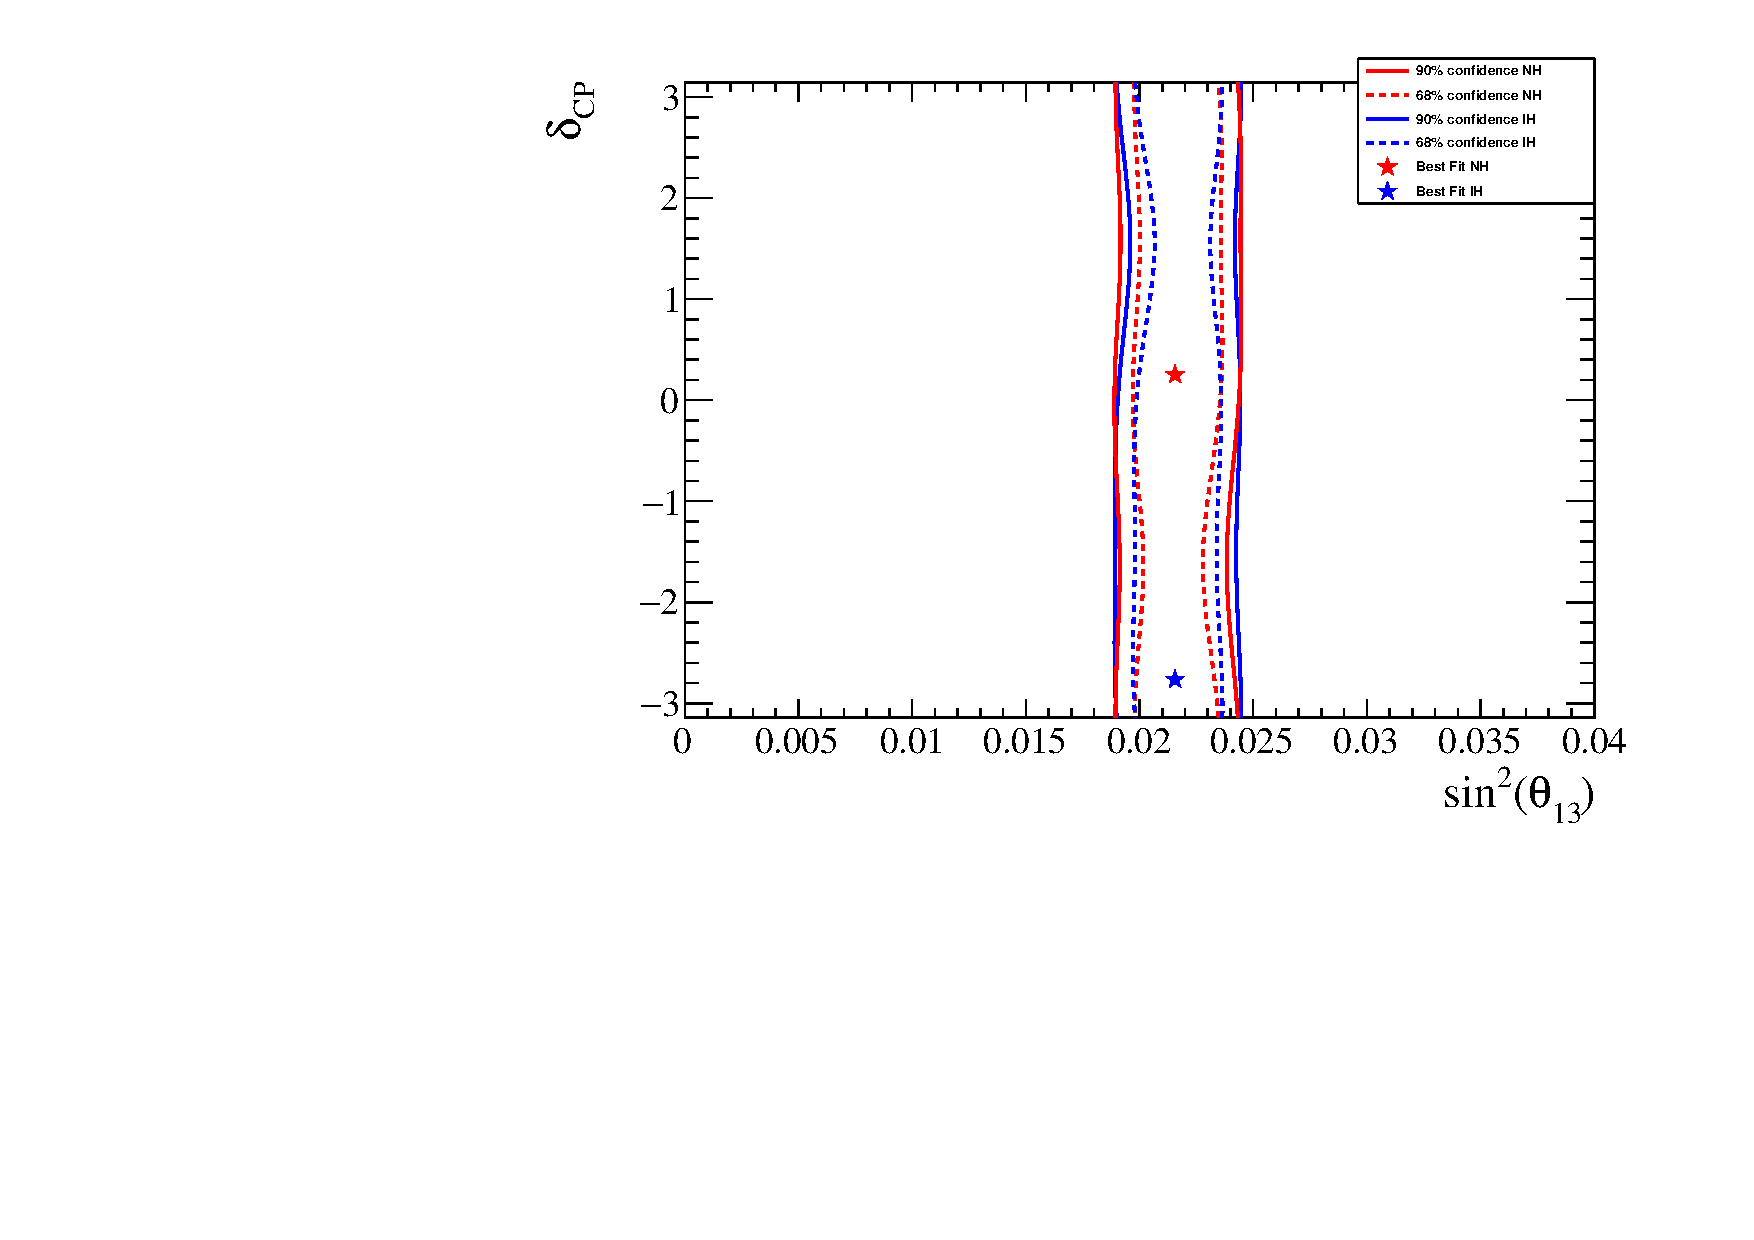
\includegraphics[width=0.9\textwidth]{./joint_plots/sensitivities/2D/cp13_reactor/cp13_reactor_B.pdf}
%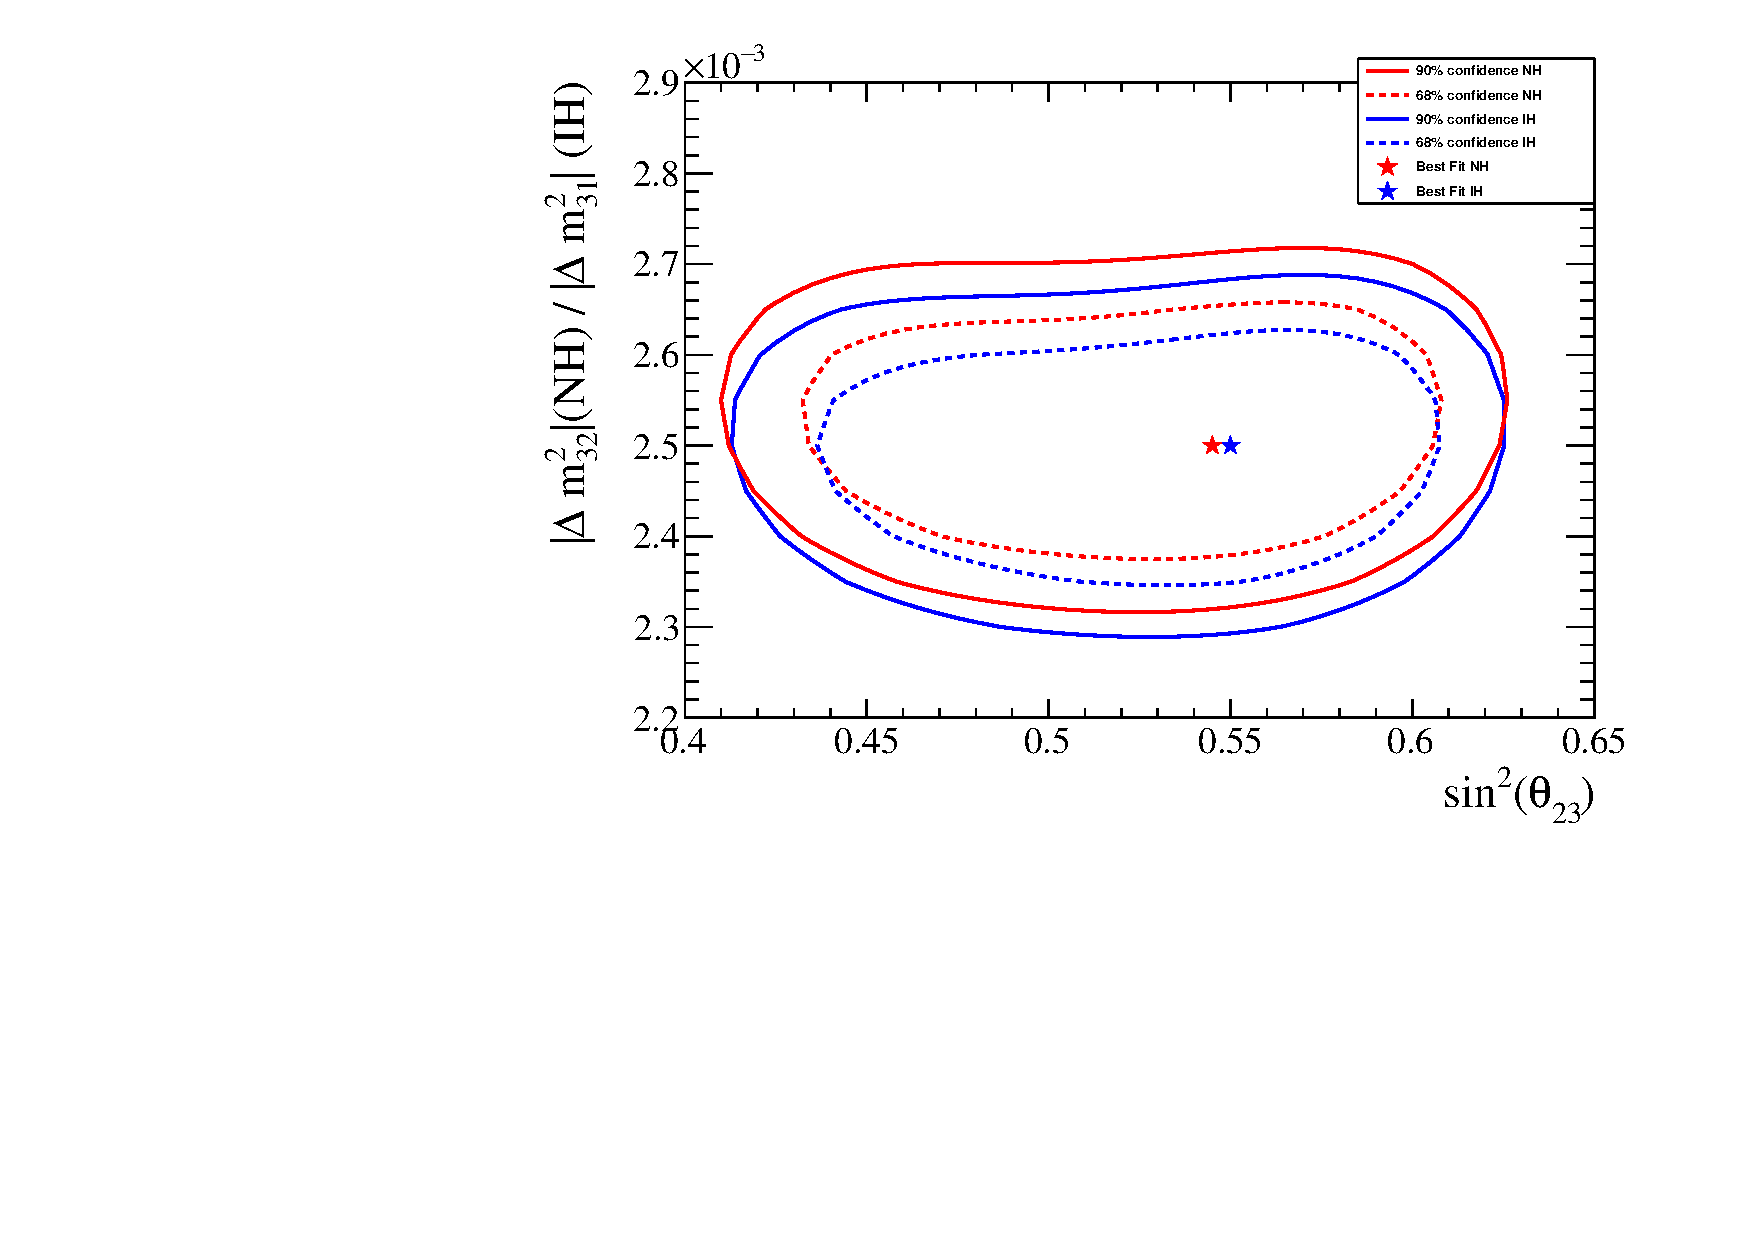
\includegraphics[width=0.9\textwidth]{./joint_plots/sensitivities/2D/ss23dmsq/ss23dmsq_A.pdf}
%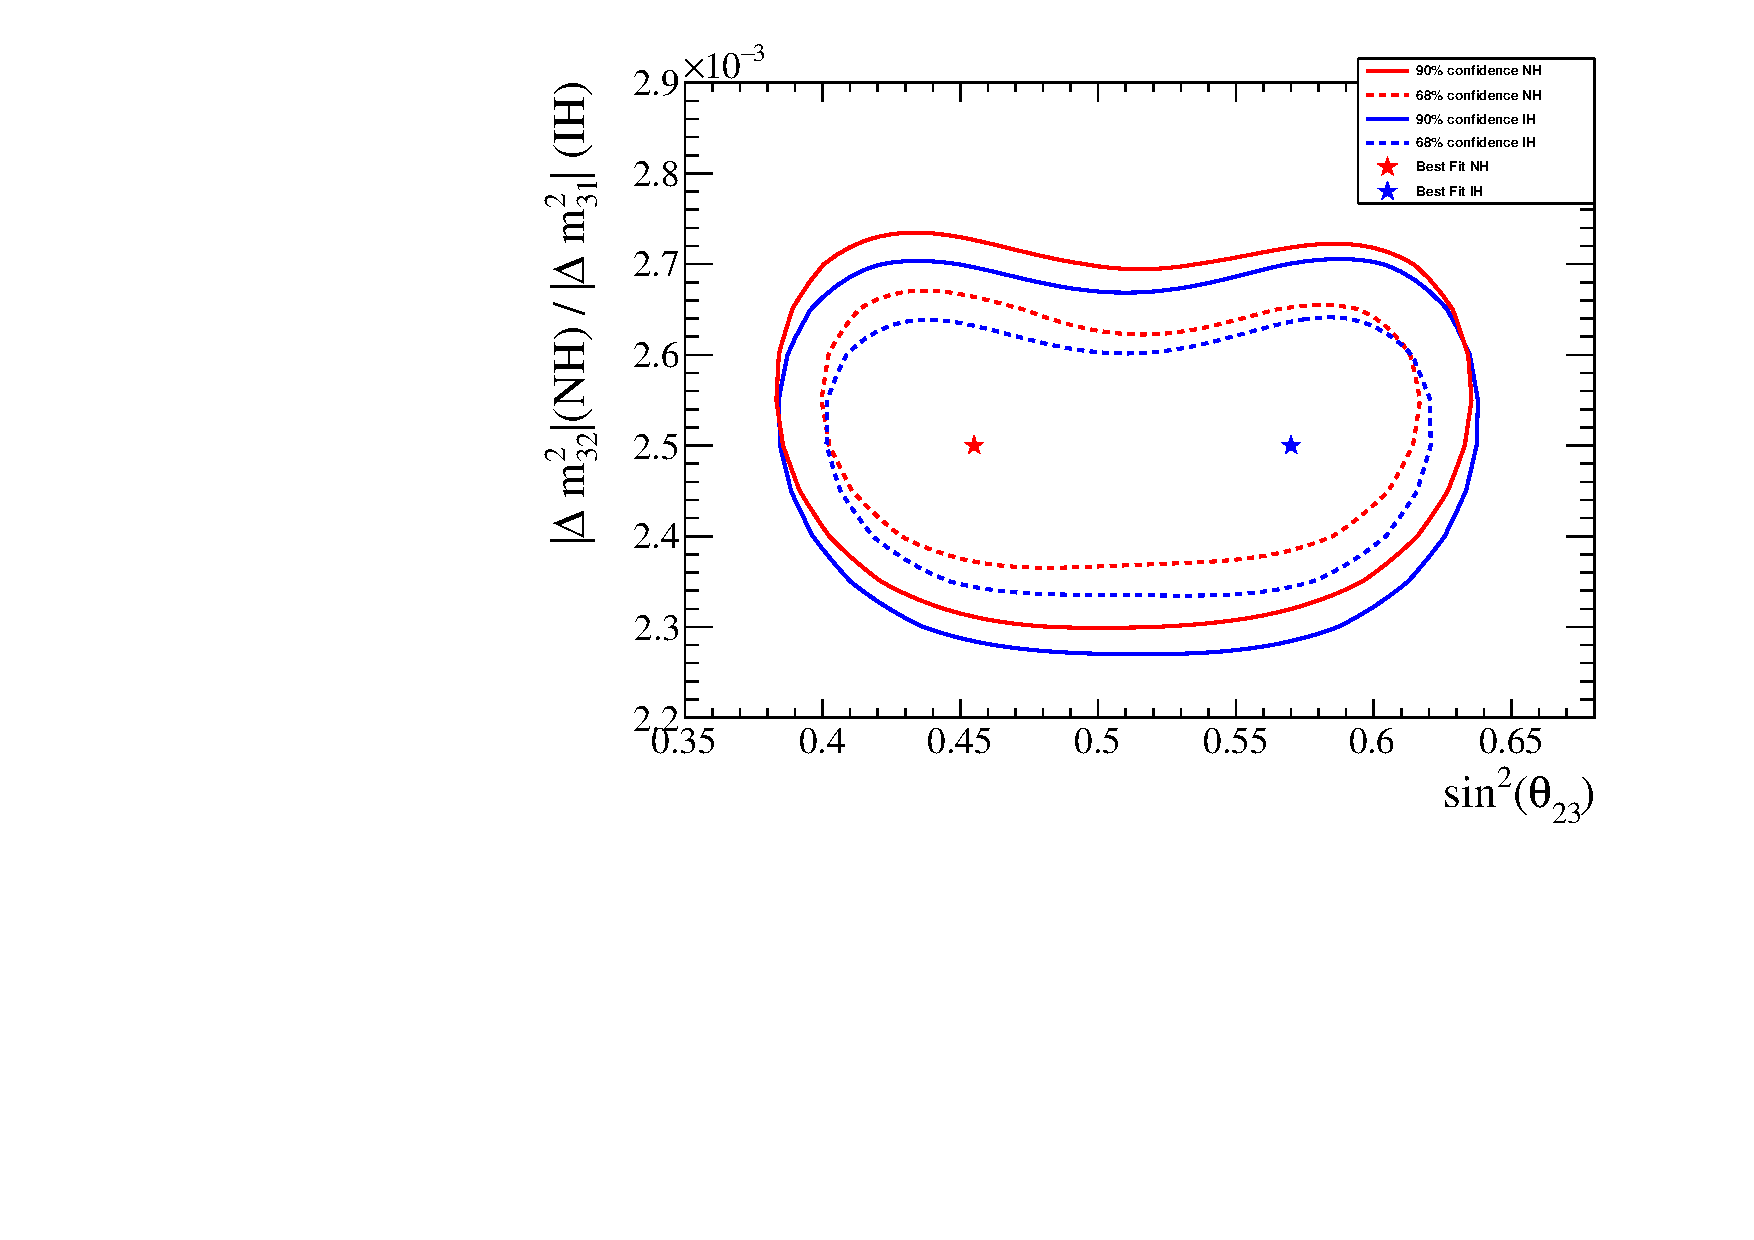
\includegraphics[width=0.9\textwidth]{./joint_plots/sensitivities/2D/ss23dmsq/ss23dmsq_B.pdf}
\begin{subfigure}[b]{0.49\textwidth}
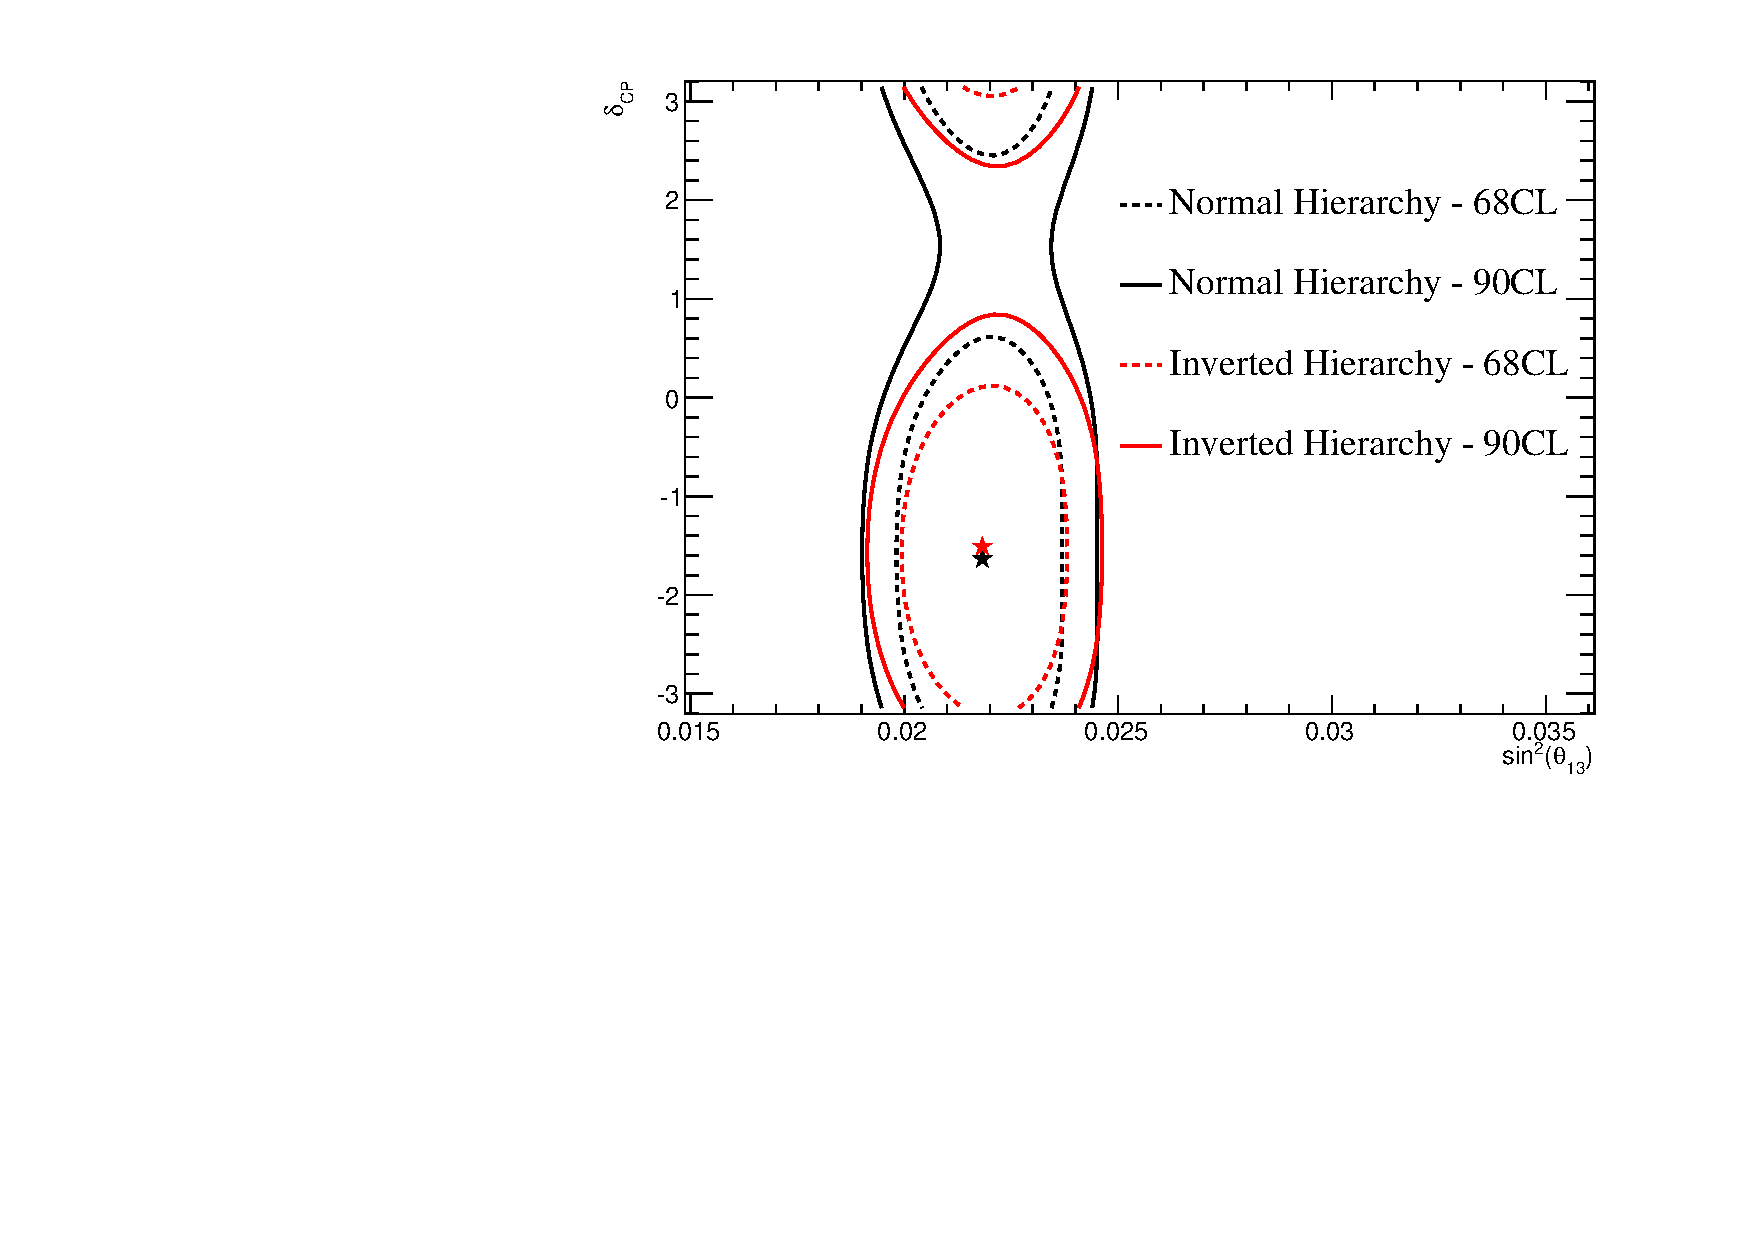
\includegraphics[width=0.9\textwidth]{./joint_plots/sensitivities/2D/contour_joint_sinsqth13Vsdcp_Asimov_A_react}
\caption{Asimov A: $\sin^2 \theta_{13}$ Vs $\delta_{CP}$. Reactor constraint.}
\end{subfigure}
\begin{subfigure}[b]{0.49\textwidth}
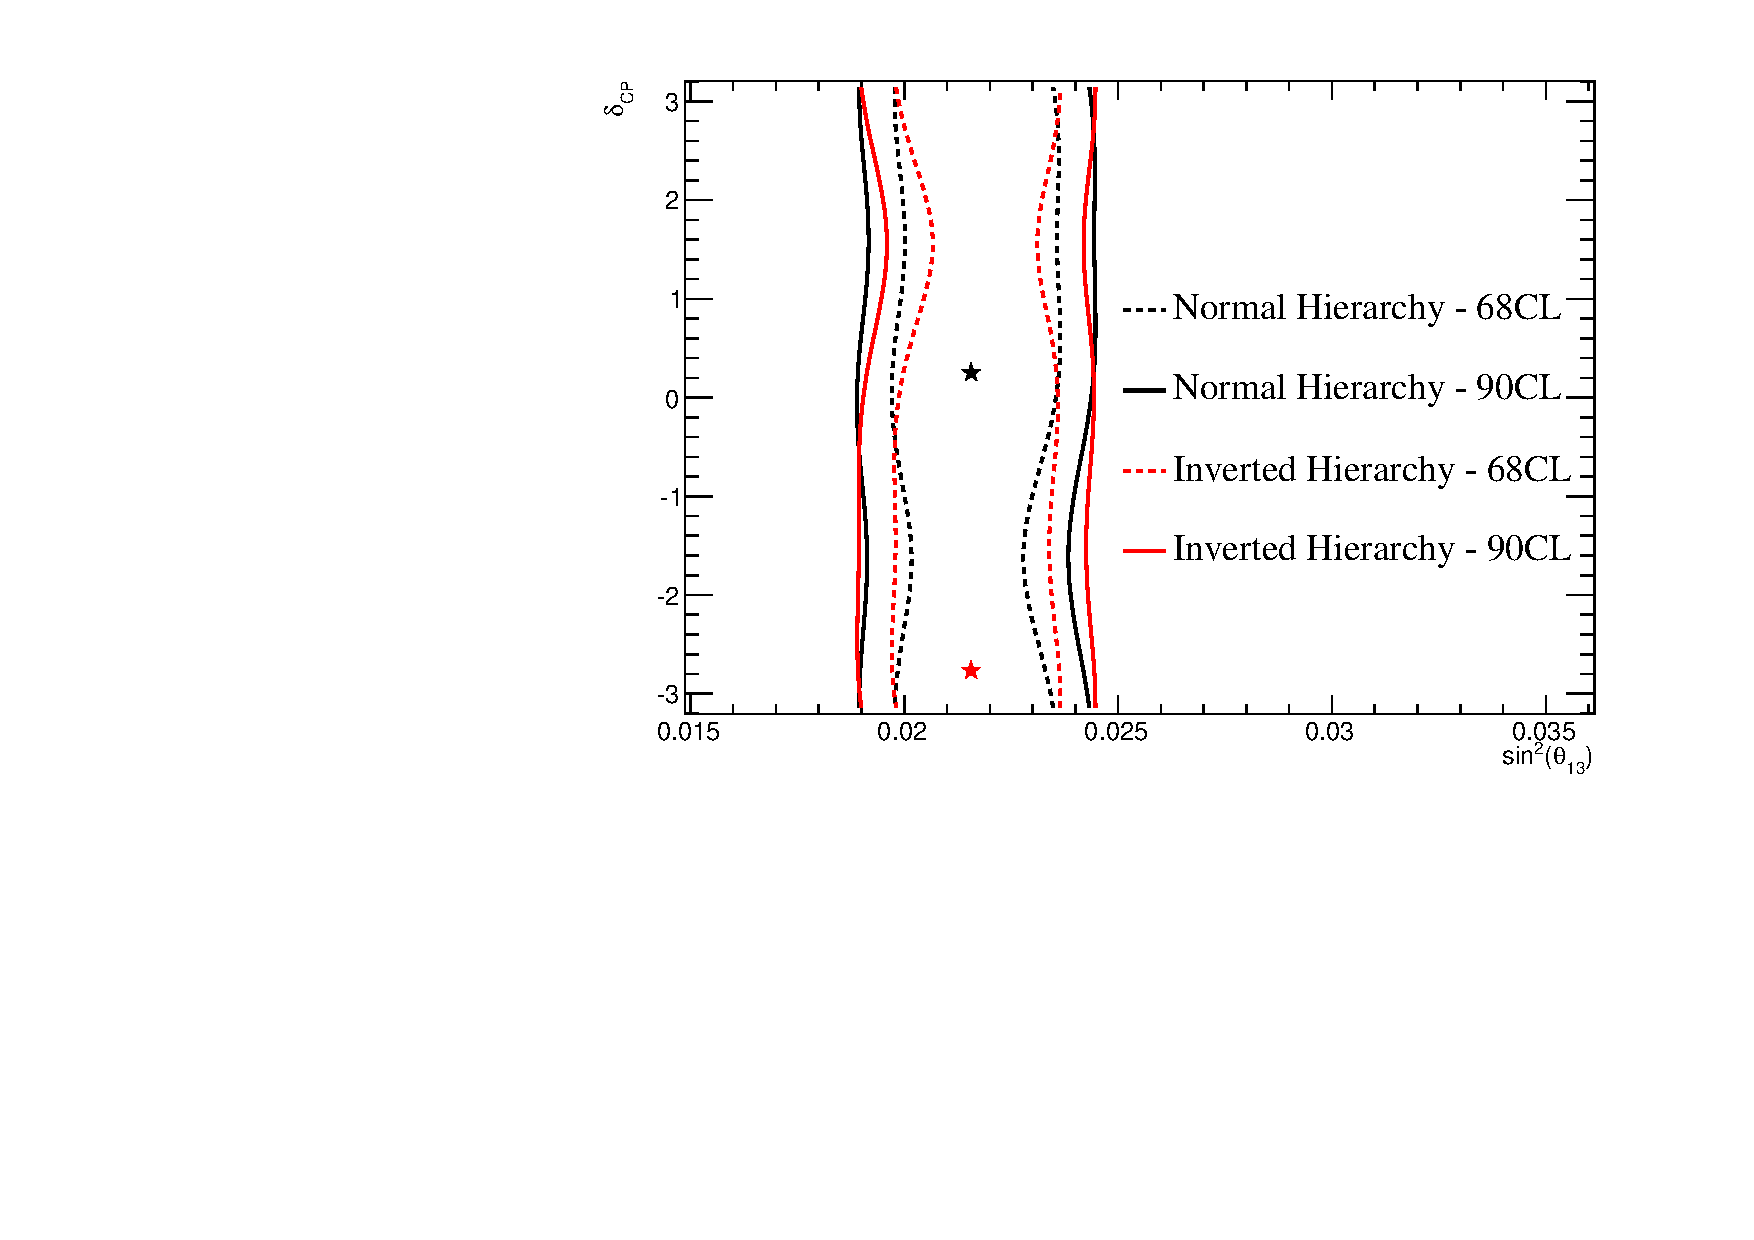
\includegraphics[width=0.9\textwidth]{./joint_plots/sensitivities/2D/contour_joint_sinsqth13Vsdcp_Asimov_B_react} 
\caption{Asimov B: $\sin^2 \theta_{13}$ Vs $\delta_{CP}$. Reactor constraint.}
\end{subfigure}
\begin{subfigure}[b]{0.49\textwidth}
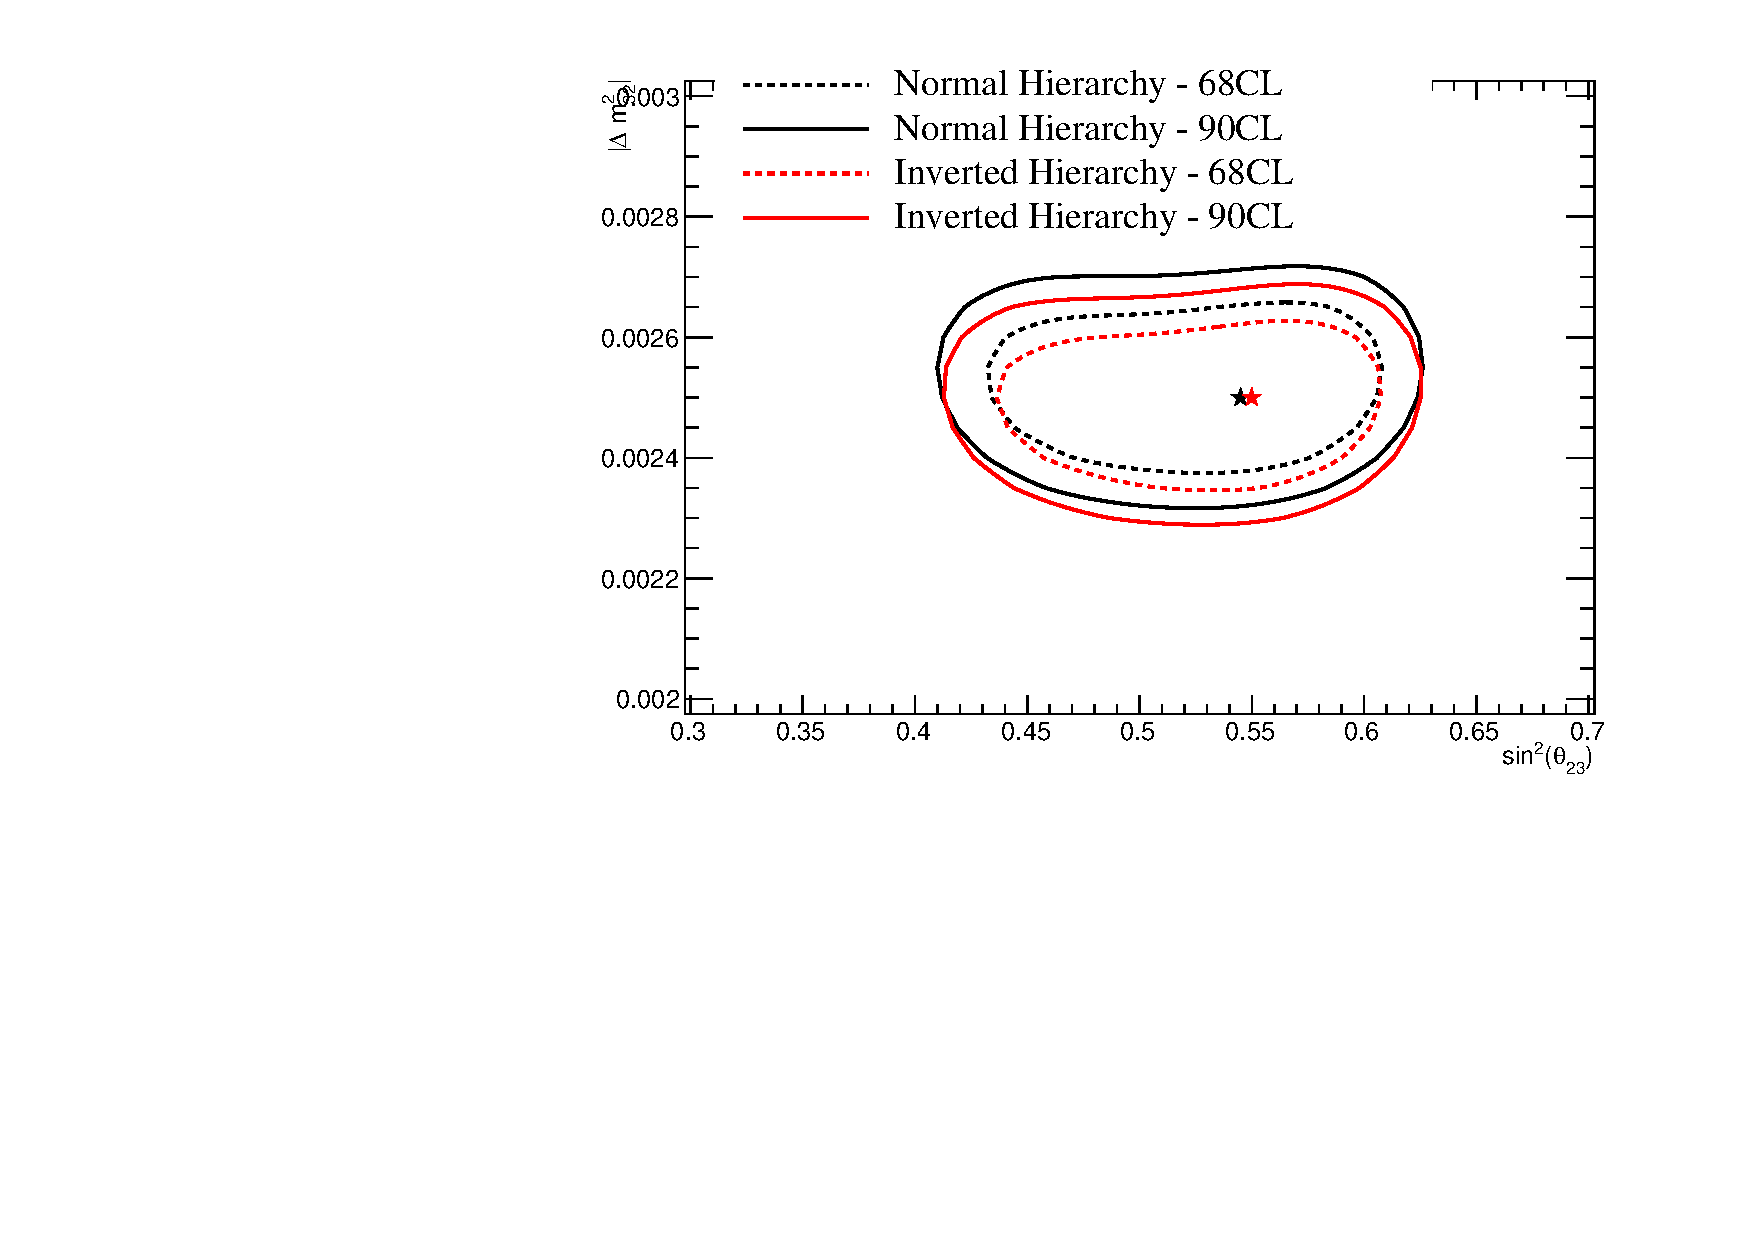
\includegraphics[width=0.9\textwidth]{./joint_plots/sensitivities/2D/contour_joint_sinsqth23Vsdmsq_Asimov_A_react}
\caption{Asimov A: $\sin^2 \theta_{23}$ Vs $\Delta m^2_{32}$ ($m^2_{13}$). Reactor constraint.}
\end{subfigure}
\begin{subfigure}[b]{0.49\textwidth}
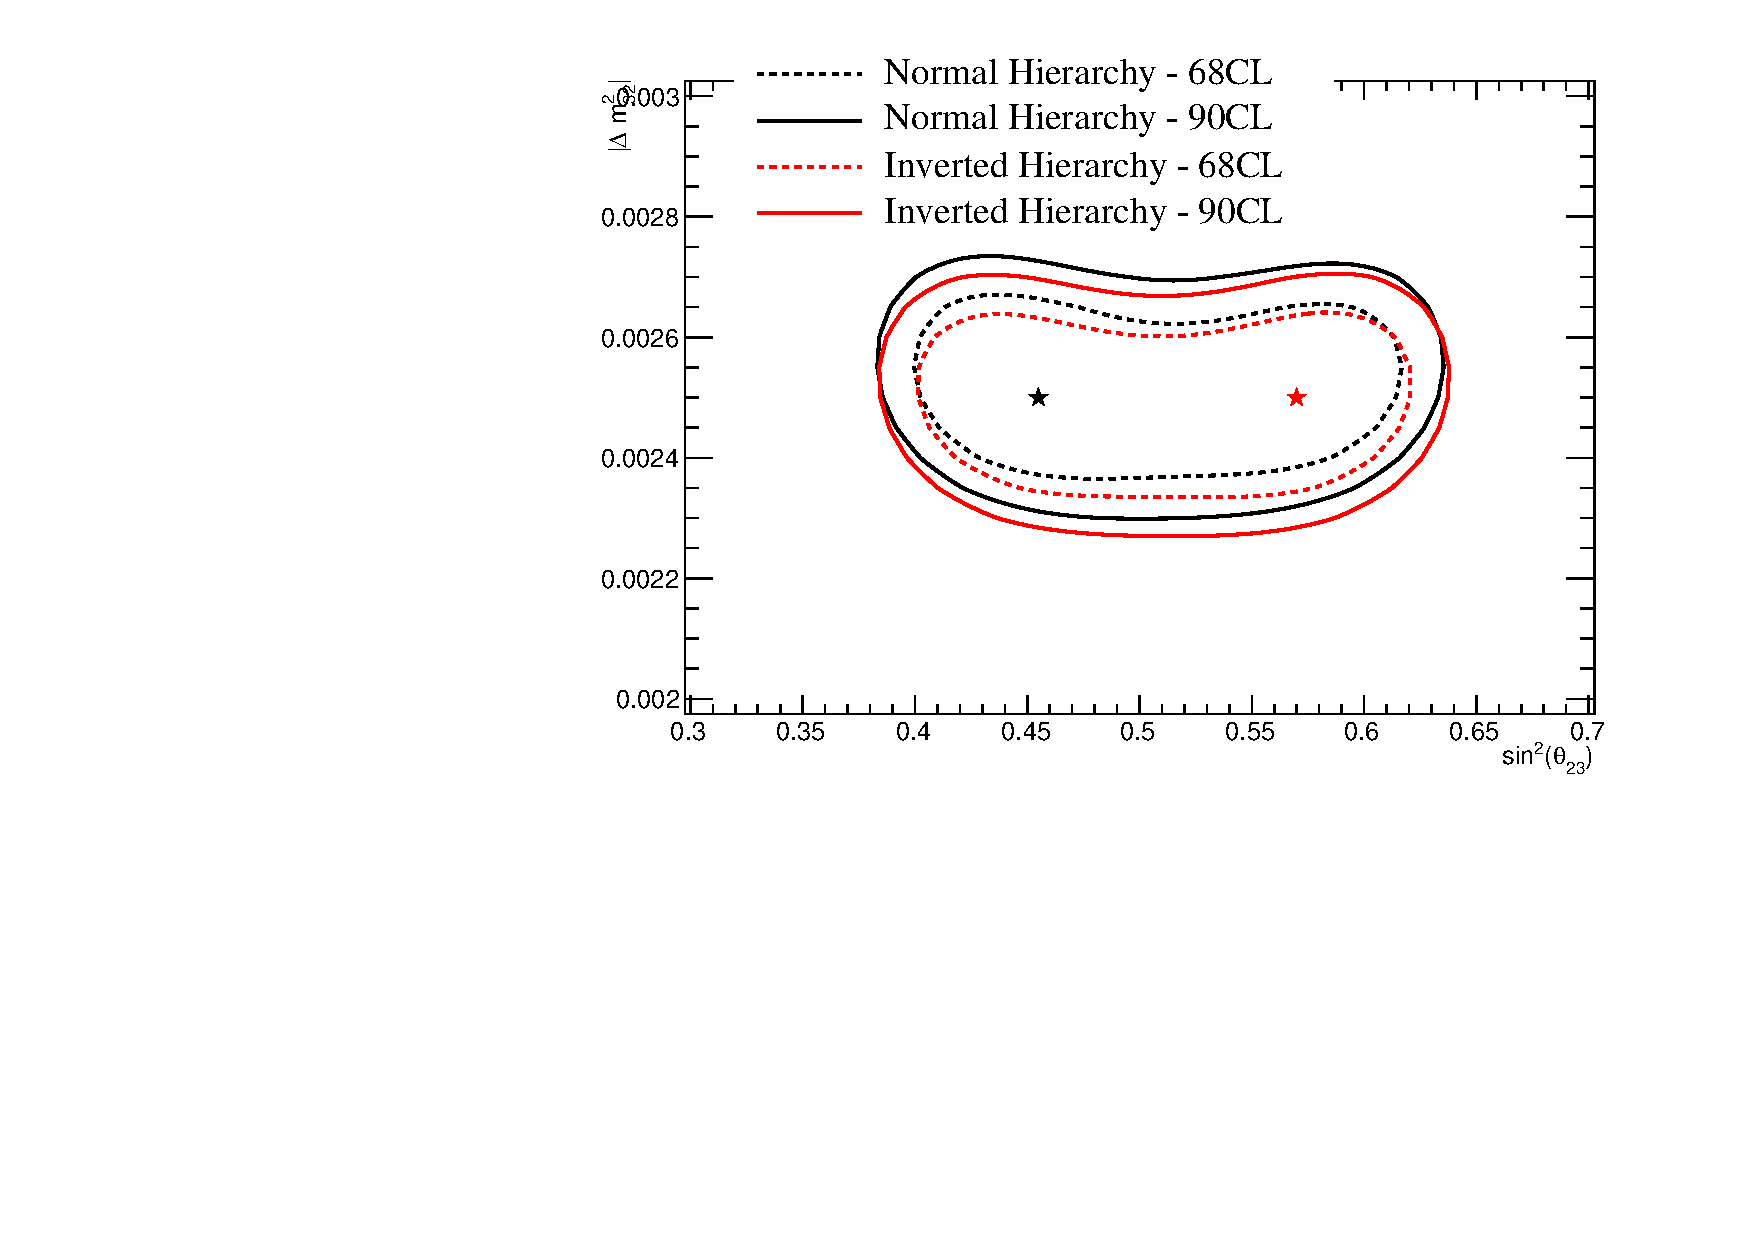
\includegraphics[width=0.9\textwidth]{./joint_plots/sensitivities/2D/contour_joint_sinsqth23Vsdmsq_Asimov_B_react}
\caption{Asimov B: $\sin^2 \theta_{23}$ Vs $\Delta m^2_{32}$ ($m^2_{13}$). Reactor constraint.}
\end{subfigure}
\caption {
%{\large{SENSI 2D CONTOURS W/ AND W/O REACTORS}}
The contours at 68\% and 90\% CL with reactor constraint 
for the Asimov data sets A and B of \cref{tab:osc_params_joint_asimov} 
corresponding to the Run 1-6 statistics 
is shown.
%is compared to the result obtained by the other analysis groups.
Normal and inverted hierarchy contours are independent.
}
\label{fig:validation_sensi_2d_reactors}
\end{figure*}

\begin{figure*}[htb]
\center
\begin{subfigure}[b]{0.49\textwidth}
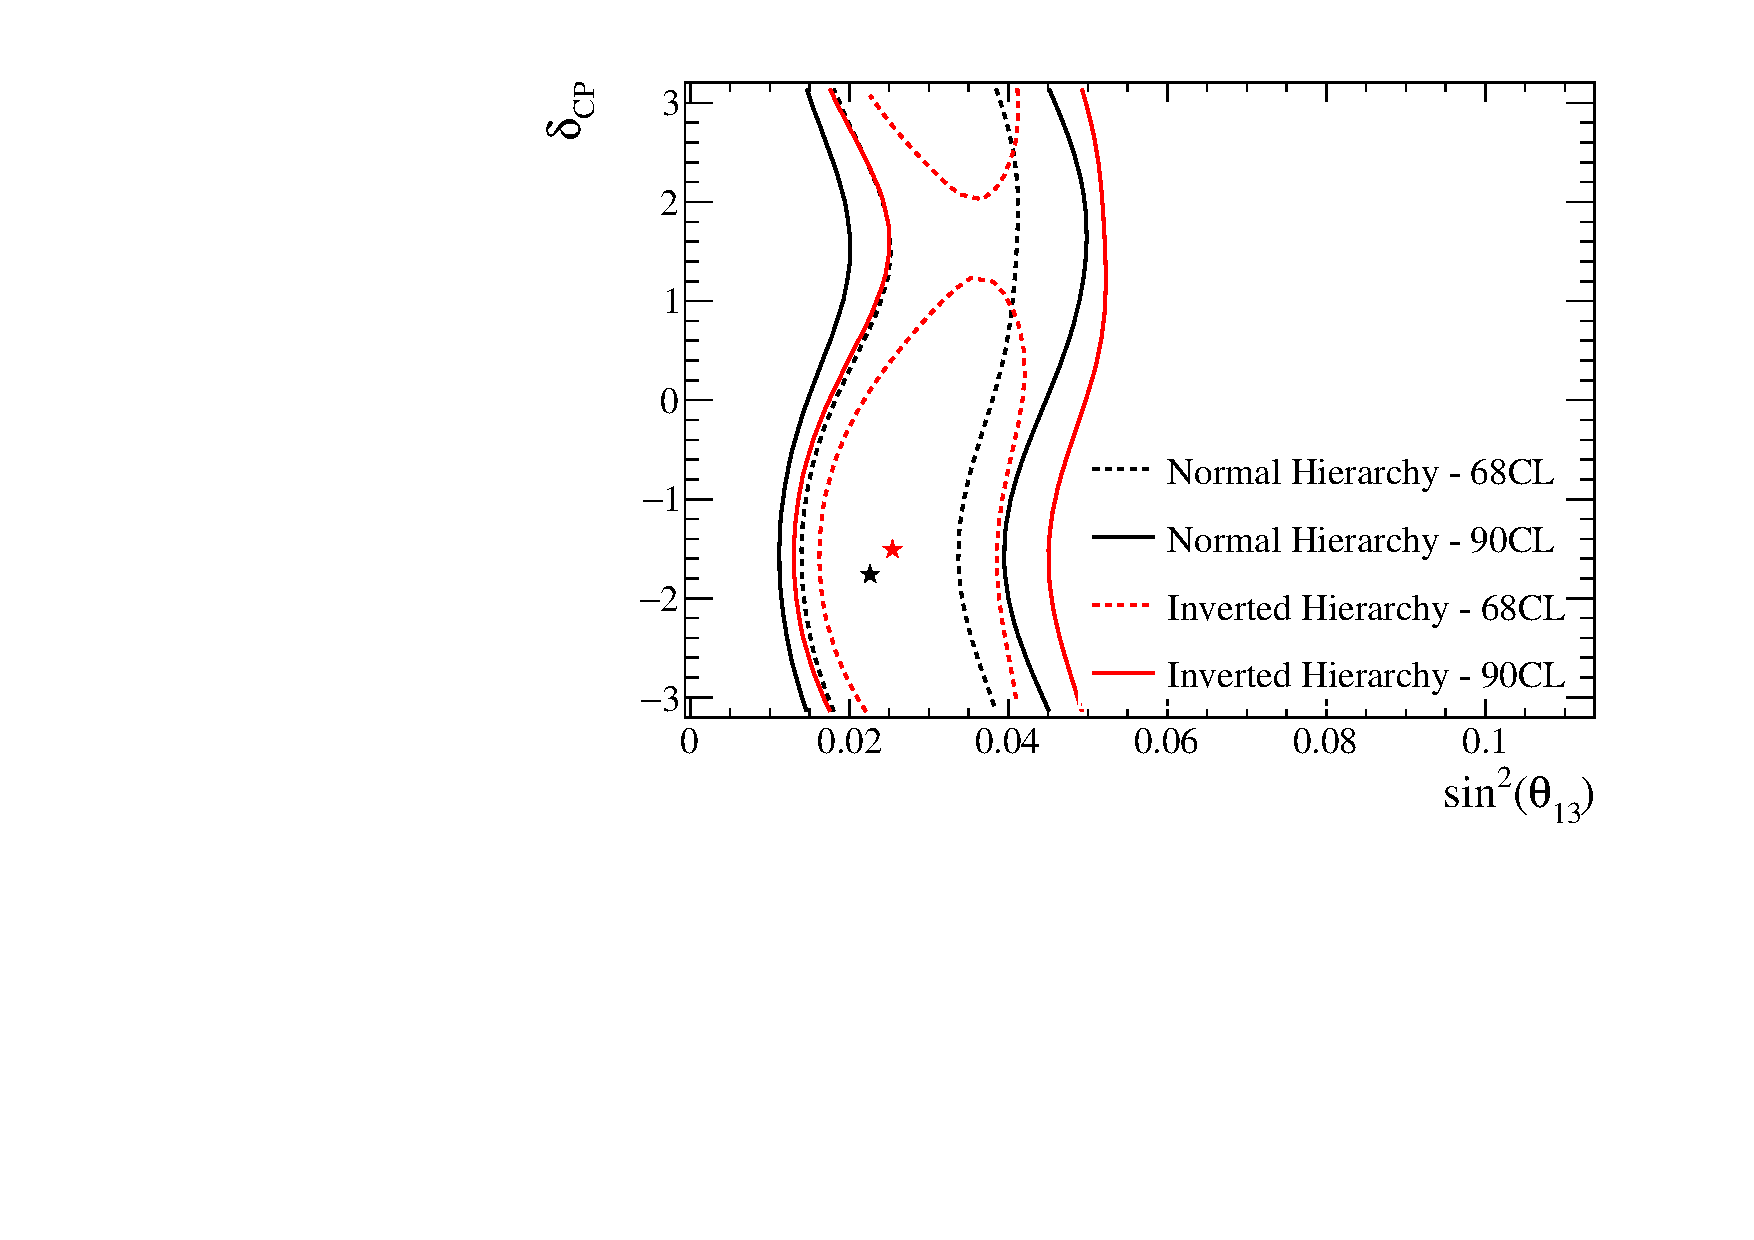
\includegraphics[width=0.9\textwidth]{./joint_plots/sensitivities/2D/cp13/cp13_A.pdf}
\caption{Asimov A with T2K data only.}
\end{subfigure}
\begin{subfigure}[b]{0.49\textwidth}
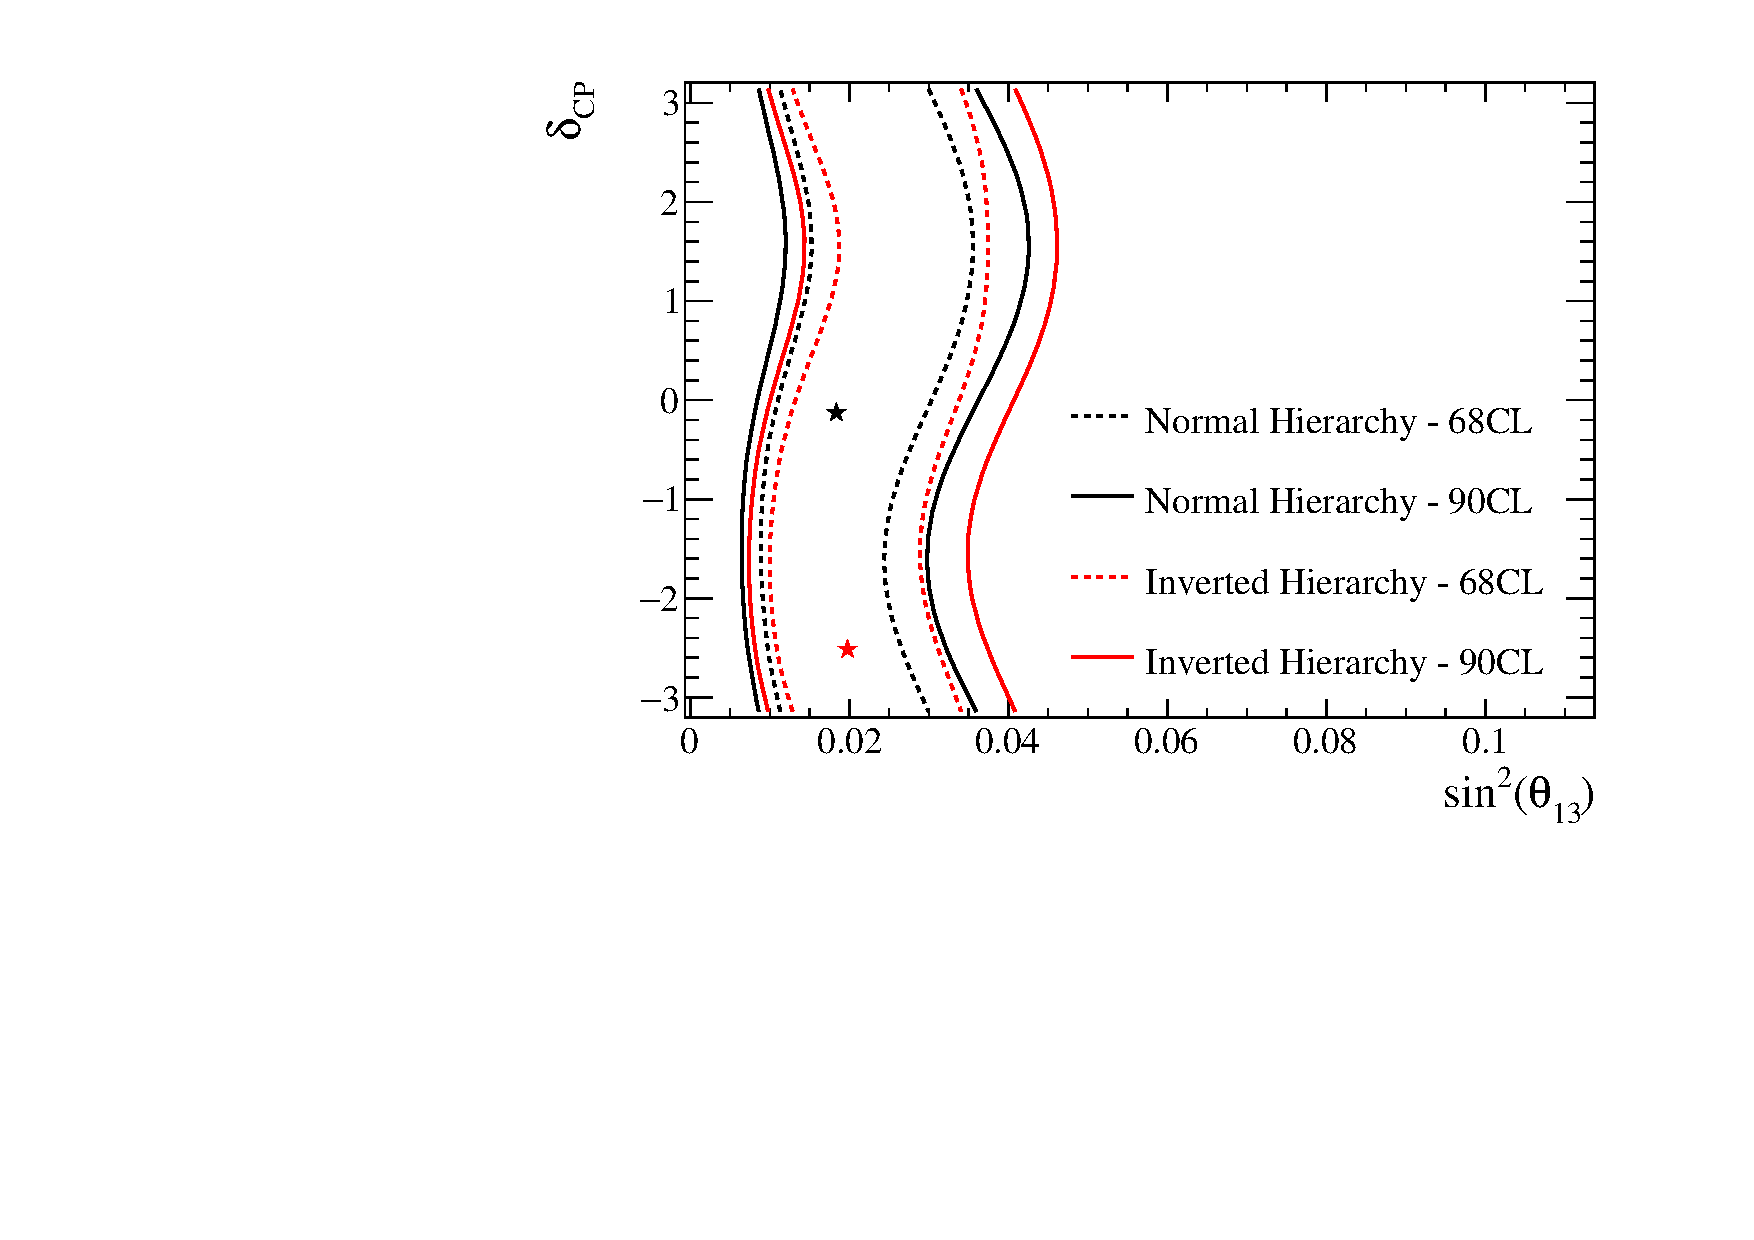
\includegraphics[width=0.9\textwidth]{./joint_plots/sensitivities/2D/cp13/cp13_B.pdf}
\caption{Asimov B with T2K data only.}
\end{subfigure}

%\begin{subfigure}[b]{0.49\textwidth}
%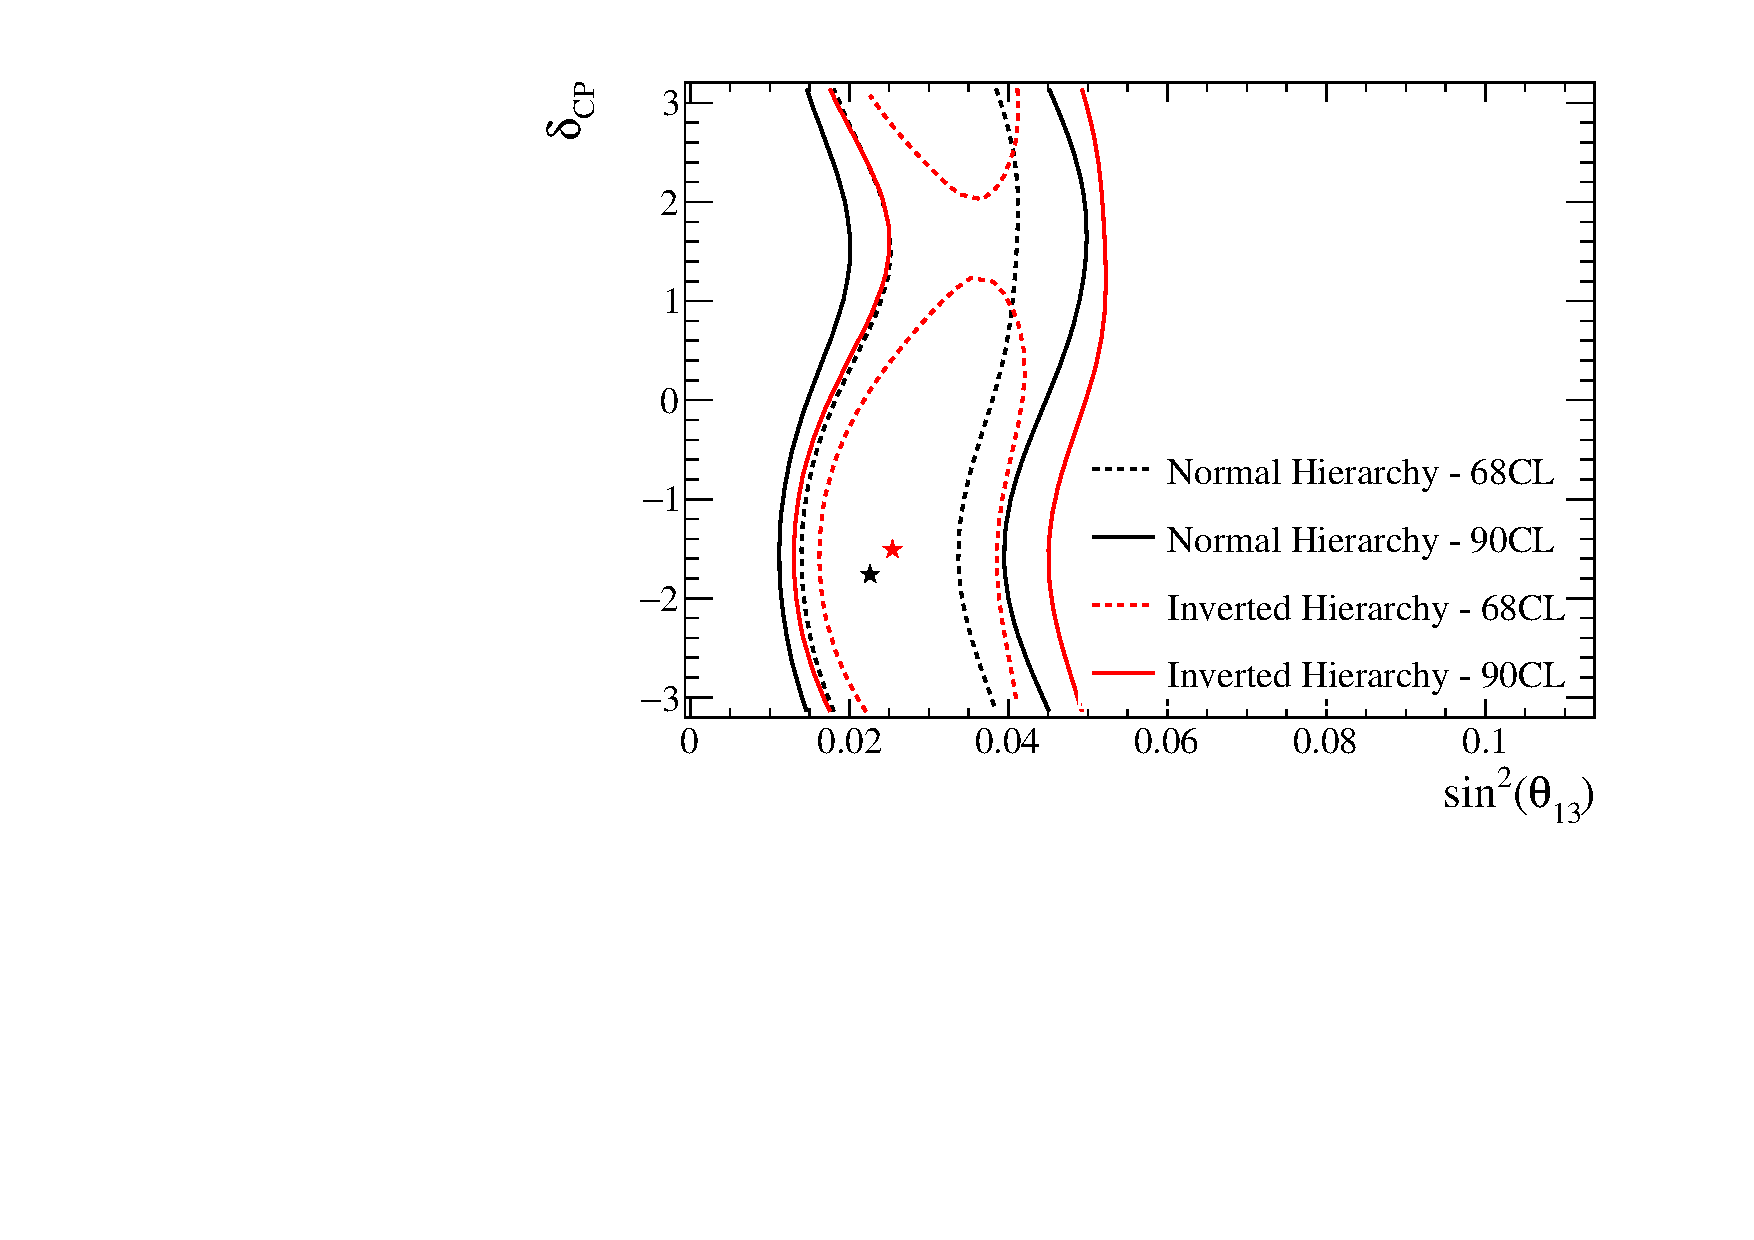
\includegraphics[width=0.9\textwidth]{./joint_plots/sensitivities/2D/cp13/cp13_A.pdf}
%\caption{Asimov A T2K only}
%\end{subfigure}
%\begin{subfigure}[b]{0.49\textwidth}
%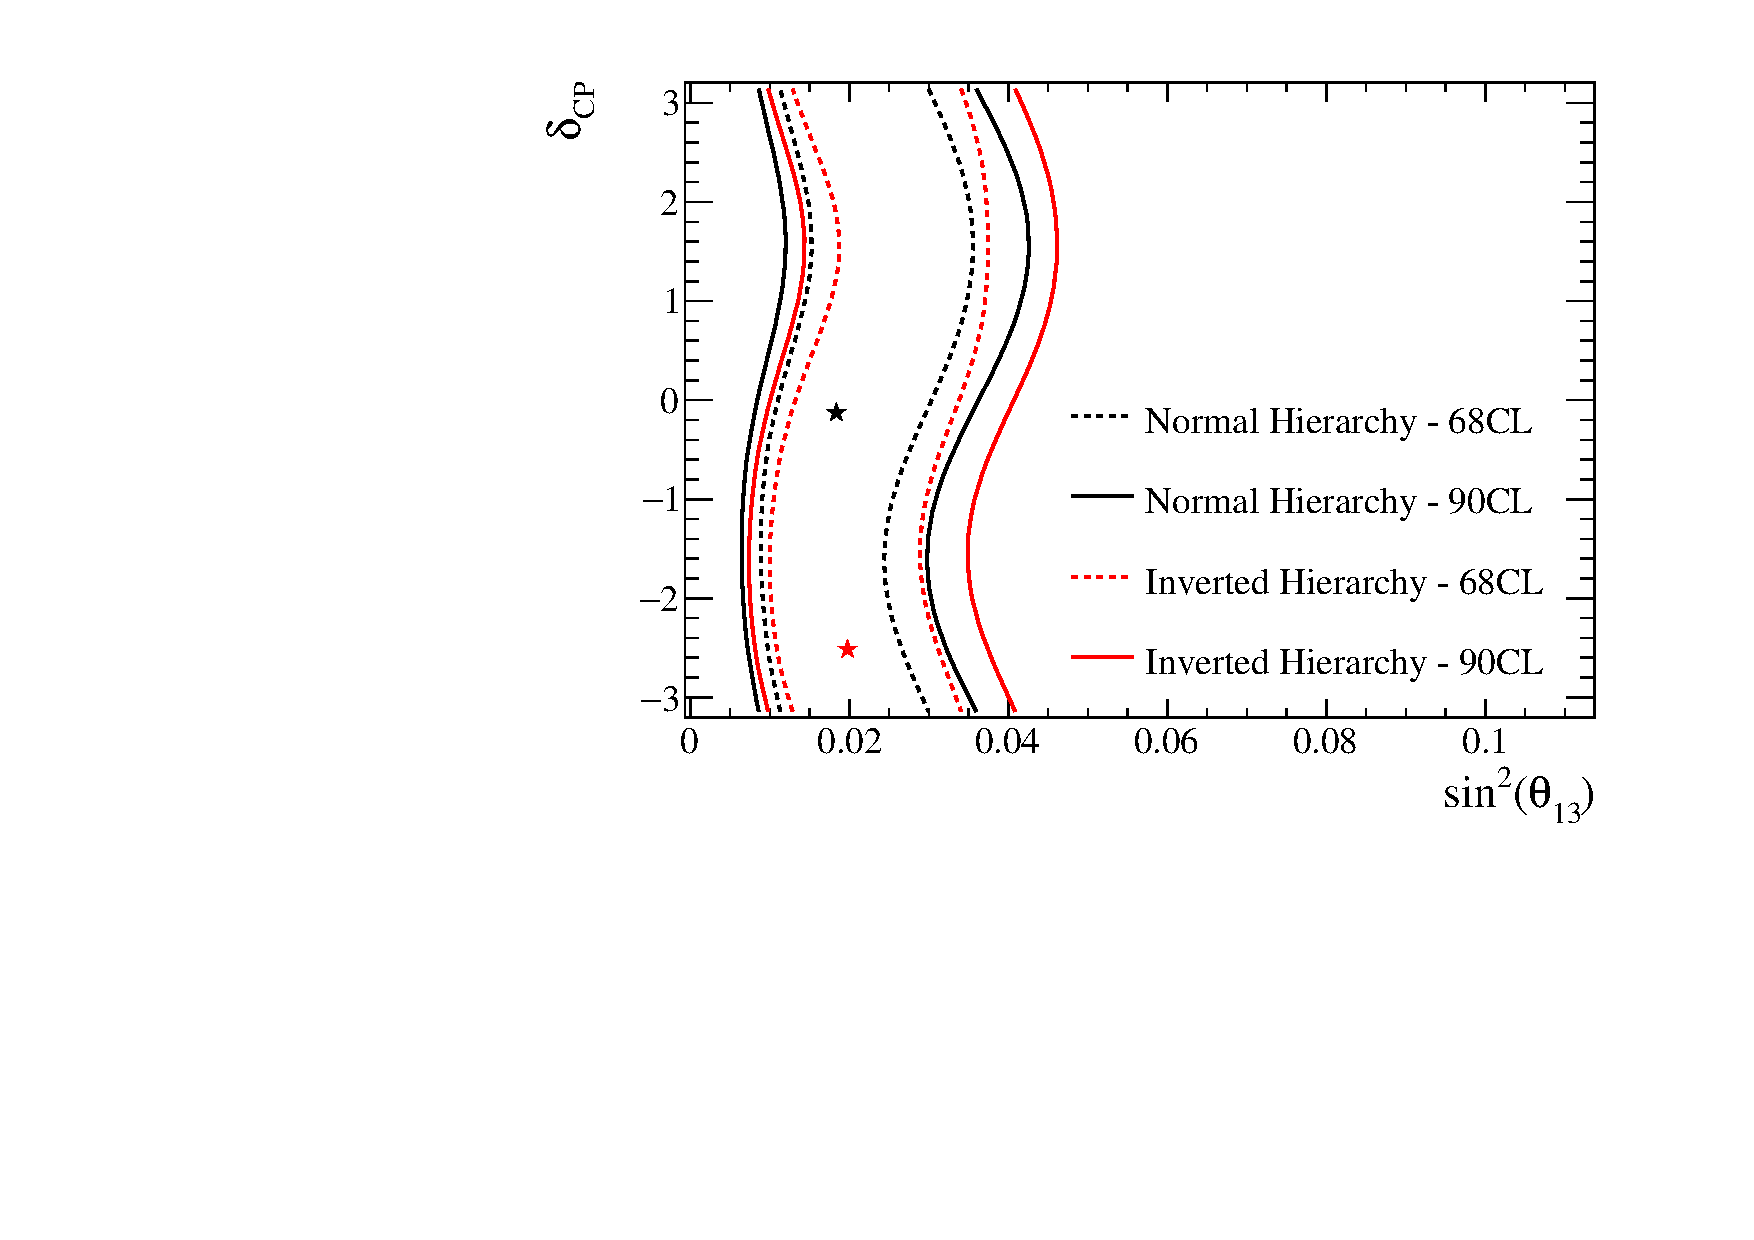
\includegraphics[width=0.9\textwidth]{./joint_plots/sensitivities/2D/cp13/cp13_B.pdf}
%\caption{Asimov B T2K only}
%\end{subfigure}

%\includegraphics[width=0.9\textwidth]{./joint_plots/sensitivities/2D/}
%\includegraphics[width=0.9\textwidth]{./joint_plots/sensitivities/2D/} \\
%\includegraphics[width=0.9\textwidth]{./joint_plots/sensitivities/2D/}
%\includegraphics[width=0.9\textwidth]{./joint_plots/sensitivities/2D/}
\caption {
%{\large{SENSI 2D CONTOURS W/ AND W/O REACTORS}}
The contours at 68\% and 90\% CL for $\sin^2 \theta_{13}$ Vs $\delta_{CP}$
for the Asimov data sets A and B of \cref{tab:osc_params_joint_asimov} 
corresponding to the Run 1-6 statistics 
is shown.
%is compared to the result obtained by the other analysis groups.
Normal and inverted hierarchy contours are independent.
Only T2K data are used.
}
\label{fig:validation_sensi_2d_t2konly}
\end{figure*}

%In Fig.~\ref{fig:validation_data_Run14_1d} and~\ref{fig:validation_data_run14_2d} 
%the same $\Delta \chi^2$ distributions for $\delta_{CP}$ 
%as well as the same contours are 
%shown for the Run 1-4 data set and compared to the other analysis groups results.
%
%\begin{figure*}[htb]
%\center
%
\includegraphics[width=0.9\textwidth]{./images/missing_plot-eps-converted-to.pdf}
%
\includegraphics[width=0.9\textwidth]{./images/missing_plot-eps-converted-to.pdf}
%\caption {
%{\large{RUN14 DELTACHISQ 1D DELTACP W/ AND W/O REACTORS}}
%The $\Delta \chi^2$ distribution as a function of $\delta_{CP}$ 
%with reactor constraint (left) and T2K only data (right) 
%for the Run 1-4 data set
%is compared to the result obtained by the other analysis groups.
%The mass hierarchy is minimized:
%both the normal and inverted hierarchy $\chi^2$ distributions 
%are shifted to the same global best-fit $\chi^2$ value,
%which is taken as the minimum between normal and inverted hierarchy.
%}
%\label{fig:validation_data_run14_1d}
%\end{figure*}
%
%\begin{figure*}[htb]
%\center
%
\includegraphics[width=0.9\textwidth]{./images/missing_plot-eps-converted-to.pdf}
%
\includegraphics[width=0.9\textwidth]{./images/missing_plot-eps-converted-to.pdf}
%
\includegraphics[width=0.9\textwidth]{./images/missing_plot-eps-converted-to.pdf}
%\caption {
%{\large{RUN14 2D CONTOURS W/ AND W/O REACTORS}}
%The contours at 68\% and 90\% CL 
%of $\sin^2 \theta_{13}$ Vs $\delta_{CP}$ 
%with reactor constraint (top left) and T2K only data (top right)
%and
%$\sin^2 \theta_{23}$ Vs $|\Delta m^2_{32}|$ 
%with reactor constraint (bottom left) and T2K only data (bottom right)
%for the Run 1-4 data set of tab.~\ref{tab:osc_params_joint} 
%is compared to the result obtained by the other analysis groups.
%Normal and inverted hierarchy contours are independent.
%}
%\label{fig:validation_data_run14_2d}
%\end{figure*}
%
%\vspace{3mm}
%{\huge{
%TODO: ADD COMMENT ON THE SENSITIVITY COMPARISONS
%}}
%\vspace{3mm}


\clearpage



%
% Coverage study of deltaCP
% 

\subsection{Coverage study of the simultaneous fit of $\delta_{CP}$ and mass hierarchy}
\label{sec:coverage_deltacp}

The fit validation is performed also by making coverage studies for the fit of 
the mass hierarchy (MH) and $\delta_{CP}$ with the reactor constraint, 
the main result of this release of the $\bar{\nu}/\nu$ joint fit,
in order to understand if the ``Feldman-Cousins method" is needed.
The coverage is defined as the number of times the true values of $\delta_{CP}^{true}$ and $\text{MH}^{true}$, used to generate the toys MC,
is contained in the confidence interval defined by \cref{eq:condition_cl}:

\begin{equation}
\Delta \chi^2 (\delta_{CP},\text{MH}) = \chi^2 (\delta_{CP}^{true},\text{MH}^{true}) - \chi^2 (\delta_{CP}^{bf},\text{MC}^{bf})
\label{eq:fc_dcp_mh}
\end{equation}

where $\delta_{CP}^{bf}$ and $\text{MH}^{bf}$ are the best-fit values.
Adopting the ``constant $\Delta \chi^2$" method, 
corresponding to the gaussian approximation,
the critical value $\Delta \chi^2_{crit} = \Delta \chi^2_{const}$, pre-computed analytically,
at a certain $X$\% confidence level is used for any value of $\delta_{CP}$ and MH.
Many toys MC are performed (10k) and for each one \cref{eq:fc_dcp_mh} is tested.
The condition used to estimate the coverage is

\begin{equation}
\Delta \chi^2 (\delta_{CP},\text{MH}) < \Delta \chi^2_{crit}
\label{eq:coverage}
\end{equation}

The fit has a good coverage if the number of toys MC
for which \cref{eq:coverage} is satisfied ($N_{toys}^{X}$)
is equal or close to $X$\% within the statistical uncertainty of the number of toys MC.
If $N_{toys}^{X} > X\%$, then the fit has over-coverage,
that means the confidence intervals should be tighter than what obtained with 
the ``constant $\Delta \chi^2$ method",
while if $N_{toys}^{X} < X\%$, then the fit has under-coverage 
and excludes a wider range of values than in the correct case.
In \cref{fig:dchisq_bestfit_dcp} the $\Delta \chi^2$ distribution
of $\delta_{CP}$ 1-dimensional fit with reactor constraint,
obtained by using \cref{eq:fc_dcp_mh},
is shown for the true values $\delta_{CP} = -\pi/2, 0, +\pi/2$.
The critical values computed using the Feldman-Cousins method are shown in 
\cref{tab:critval_0_pmhalfpi}.
It can be seen that the coverage given by the constant critical values is not correct,
so, in order to provide correct confidence intervals, the Feldman-Cousins method is required. 


\begin{figure*}[htb]
\center
\begin{subfigure}[b]{0.49\textwidth}
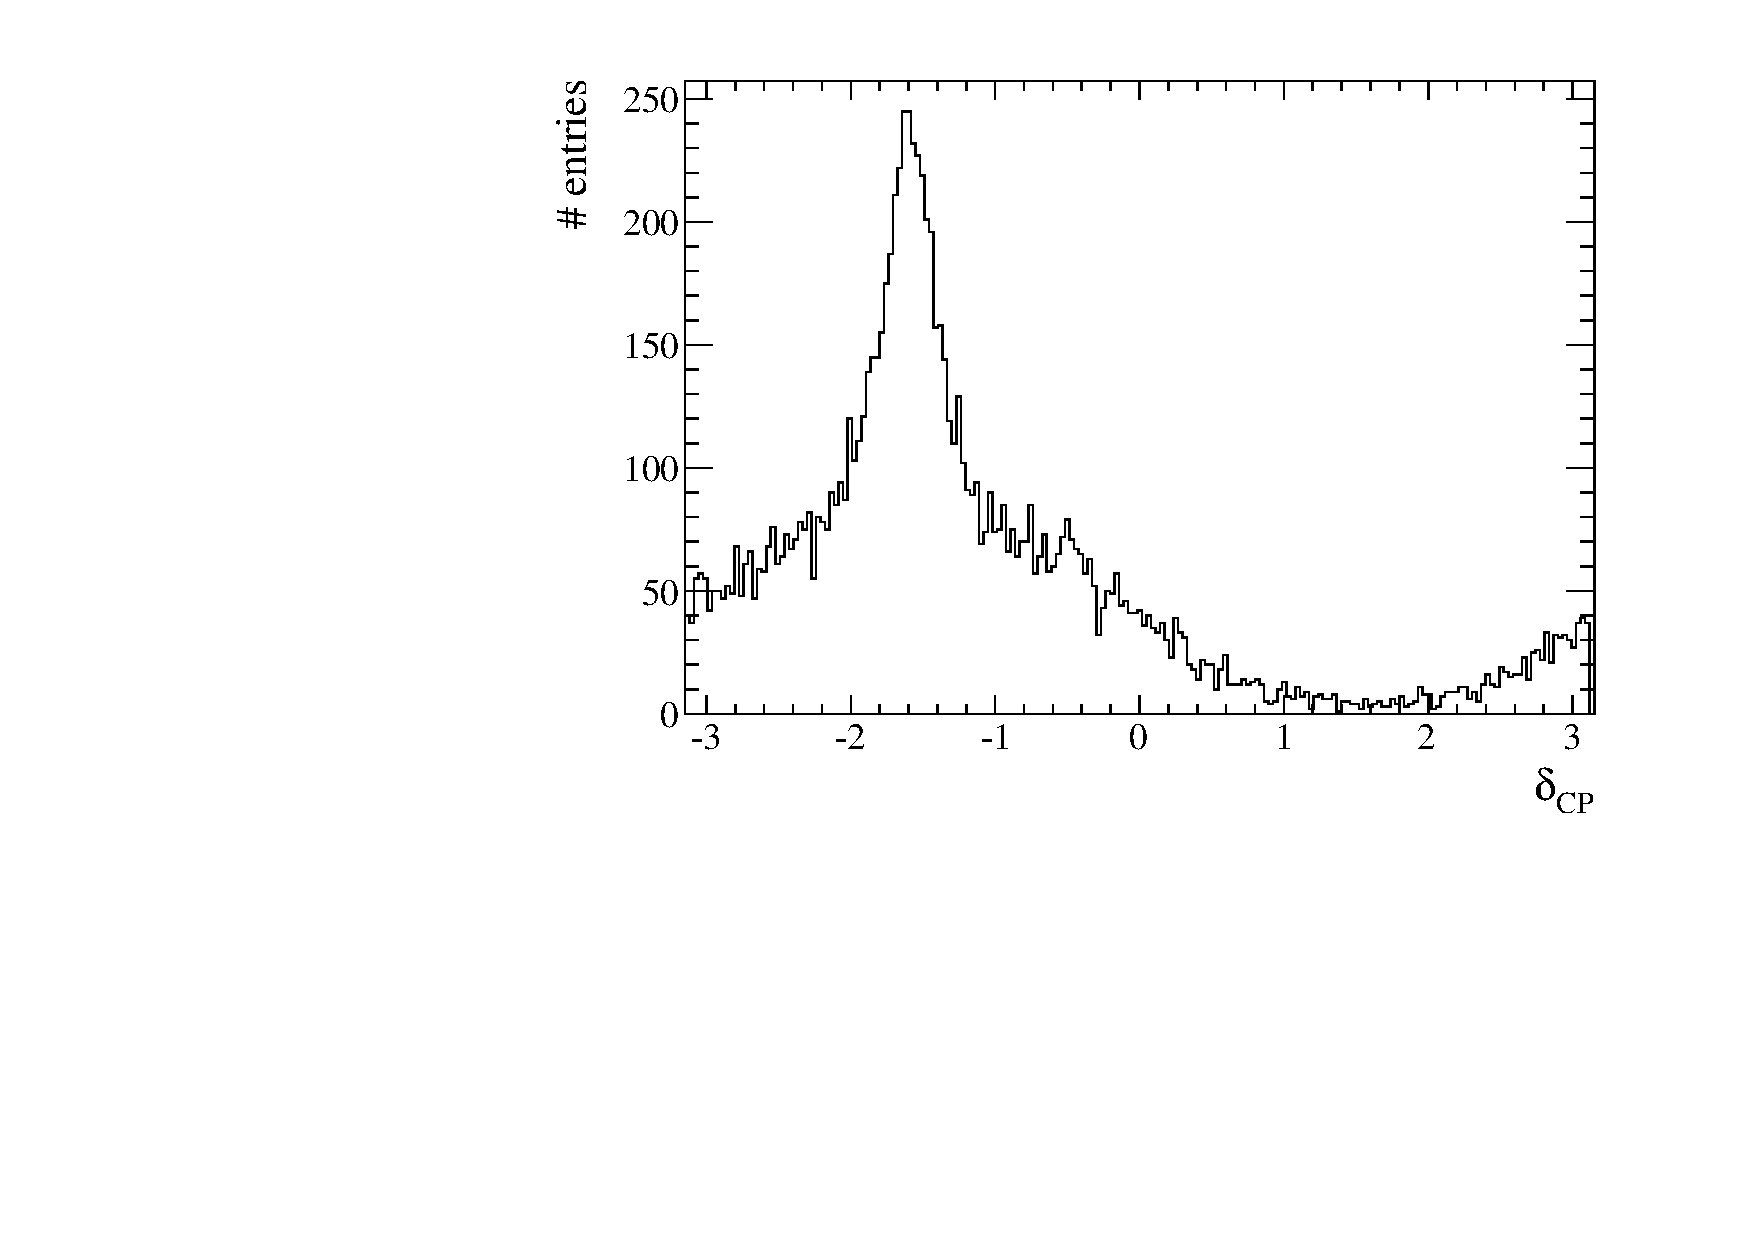
\includegraphics[width=0.9\textwidth]{./joint_plots/coverage_fc/coverage/cbestfit_deltacp_-1p571_1D_normal.pdf}
\caption{Best-fit distribution of $\delta_{CP}$. $\delta_{CP}^{true} = -\pi/2$.}
\end{subfigure}
\begin{subfigure}[b]{0.49\textwidth}
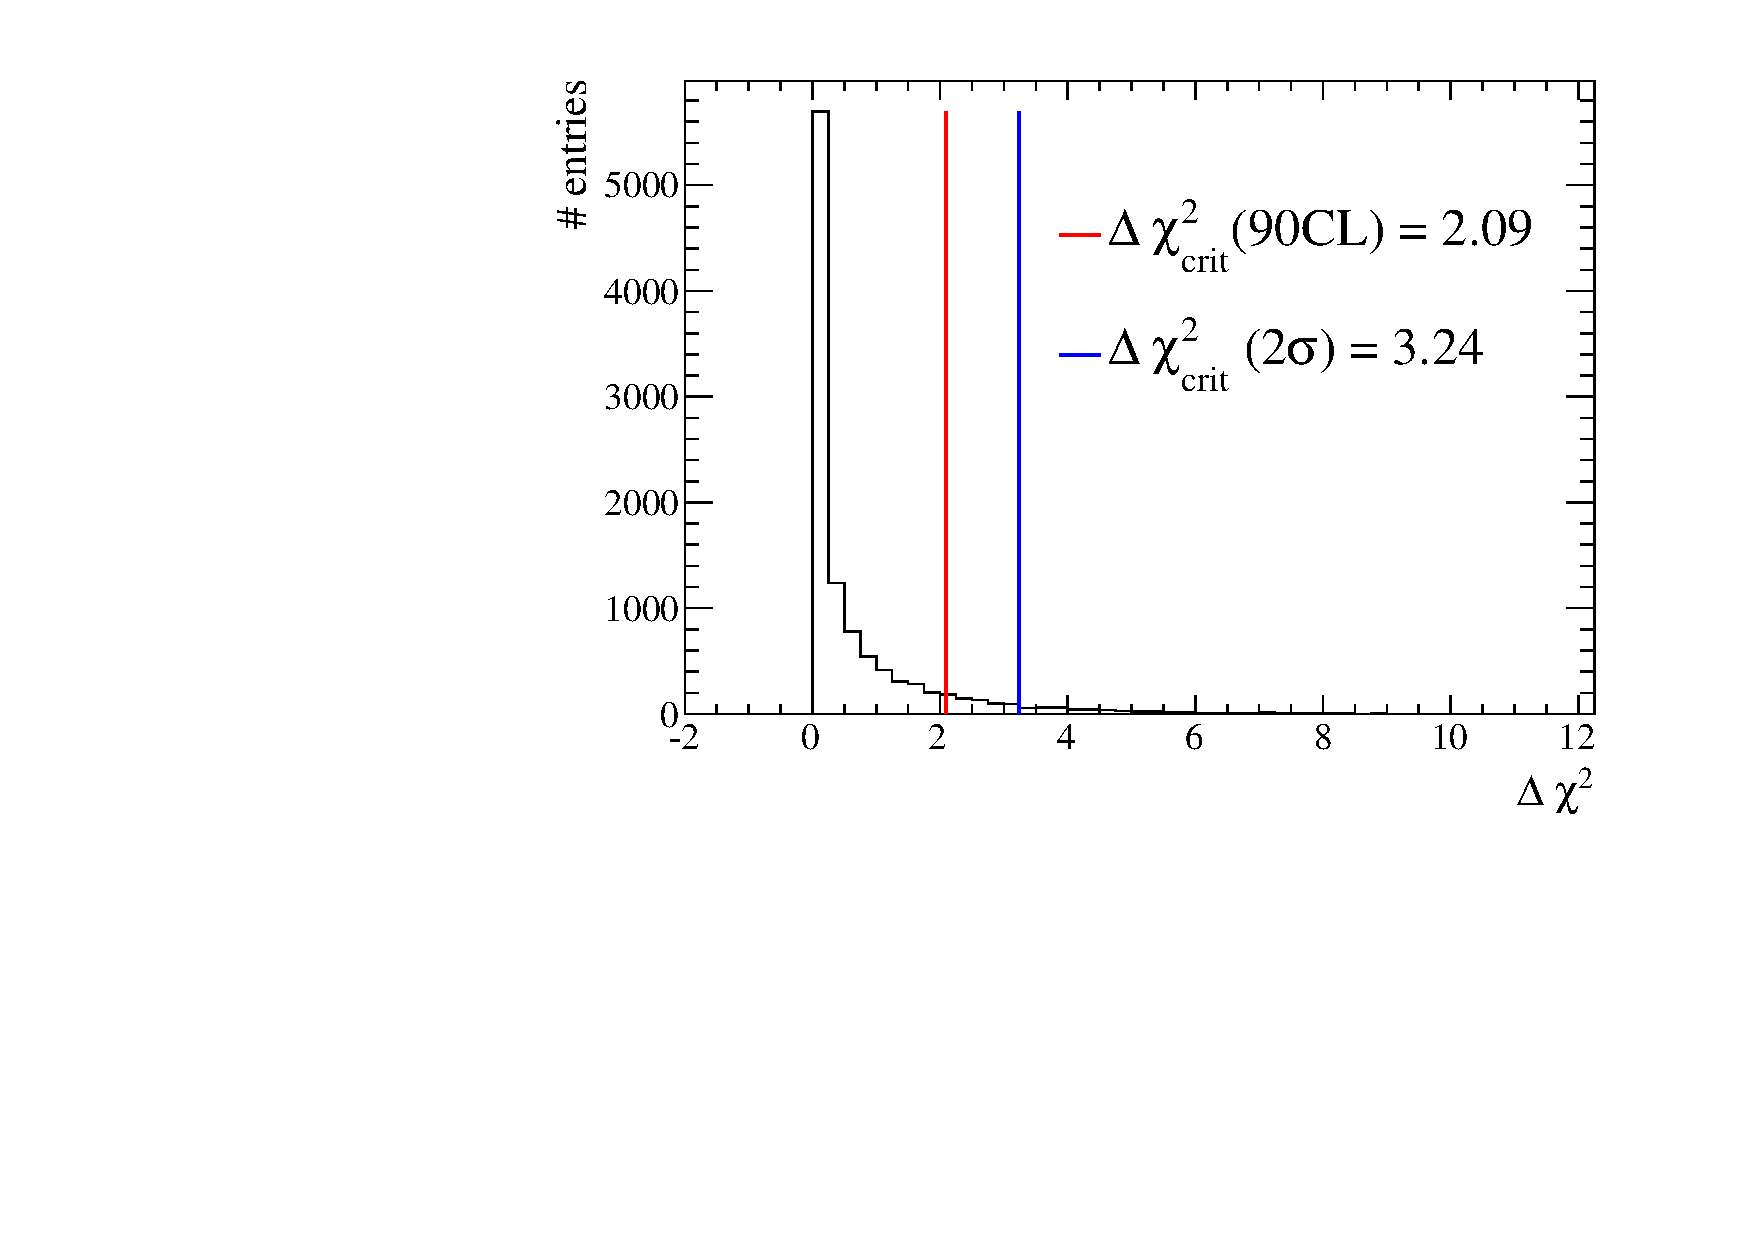
\includegraphics[width=0.9\textwidth]{./joint_plots/coverage_fc/coverage/deltachisq_glob_deltacp_-1p571_1D_normal.pdf}
\caption{$\Delta \chi^2$ distribution.
$\delta_{CP}^{true} = -\pi/2$.}
\end{subfigure}
\begin{subfigure}[b]{0.49\textwidth}
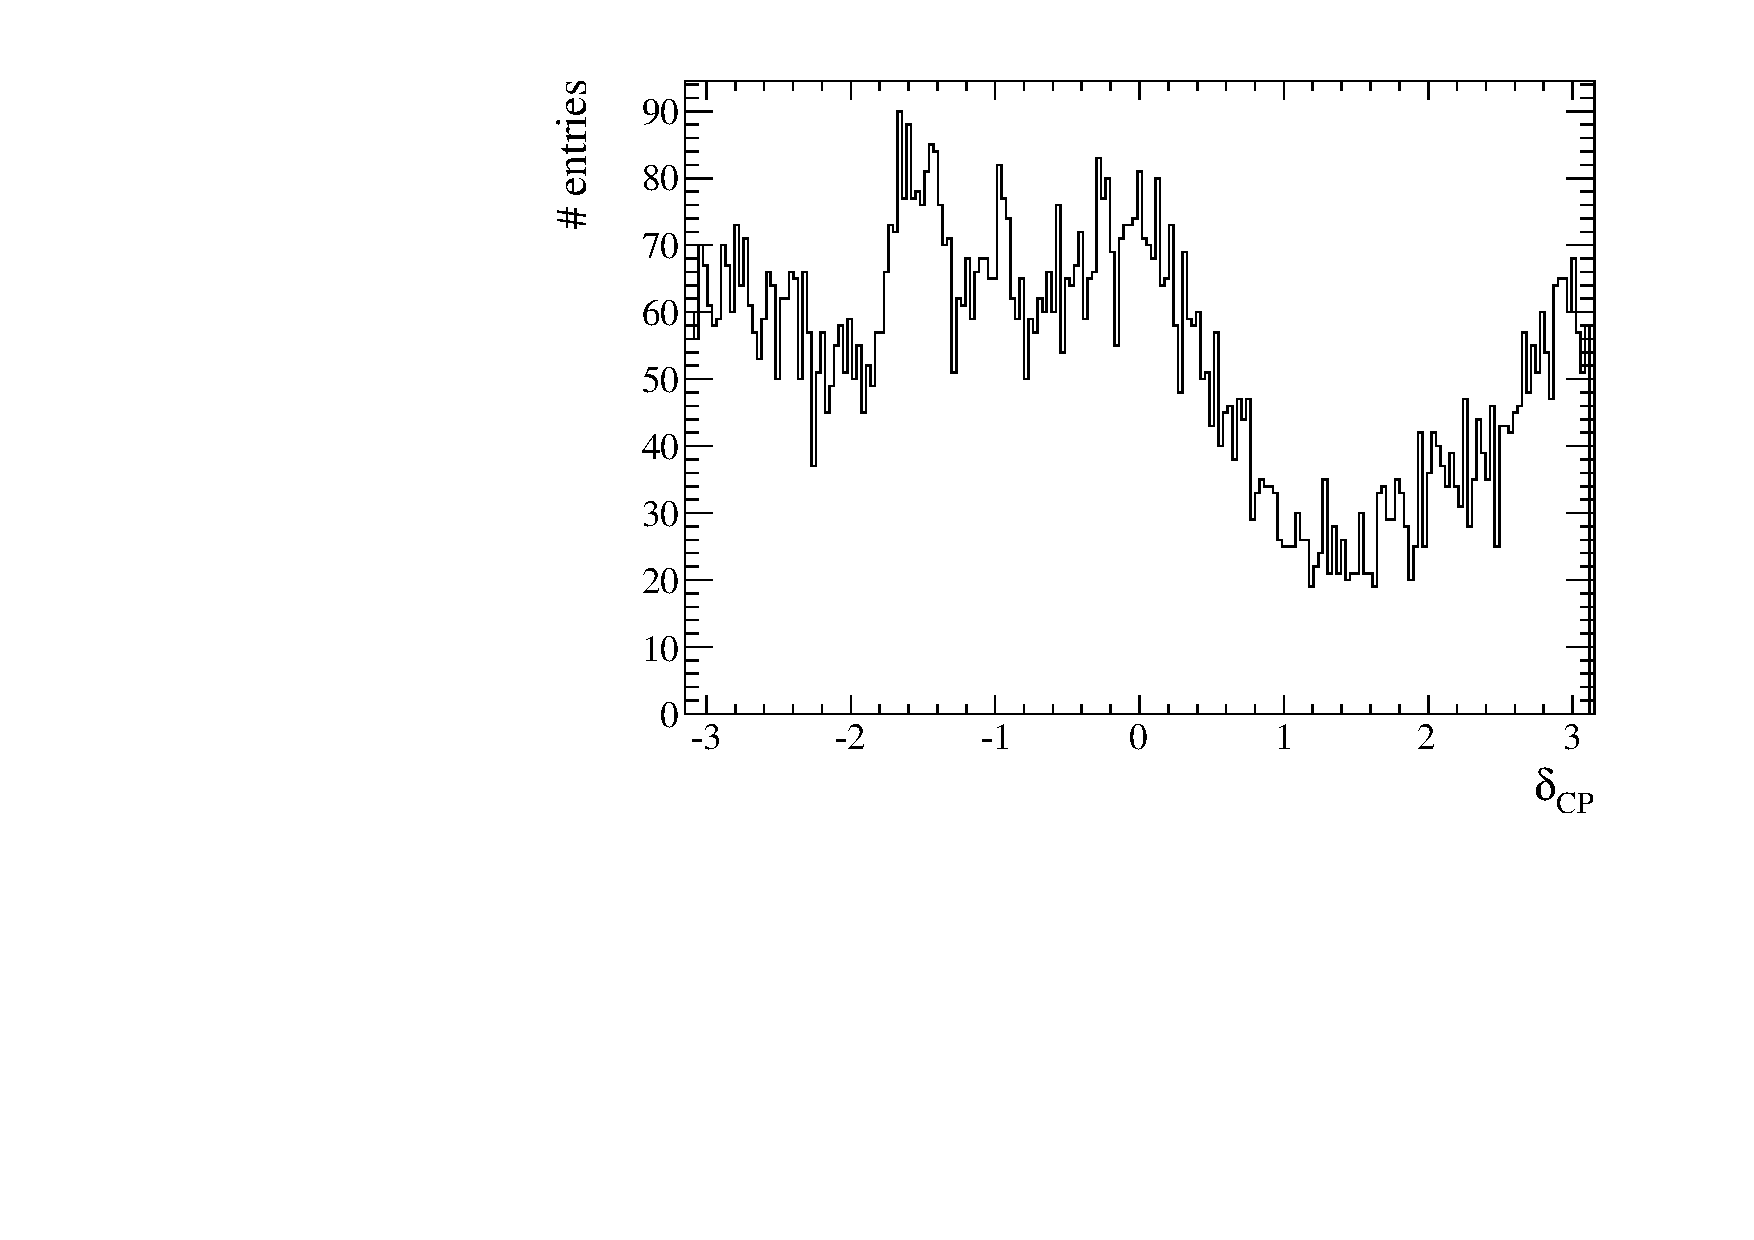
\includegraphics[width=0.9\textwidth]{./joint_plots/coverage_fc/coverage/cbestfit_deltacp_0_1D_normal.pdf}
\caption{Best-fit distribution of $\delta_{CP}$. $\delta_{CP}^{true} = 0$.}
\end{subfigure}
\begin{subfigure}[b]{0.49\textwidth}
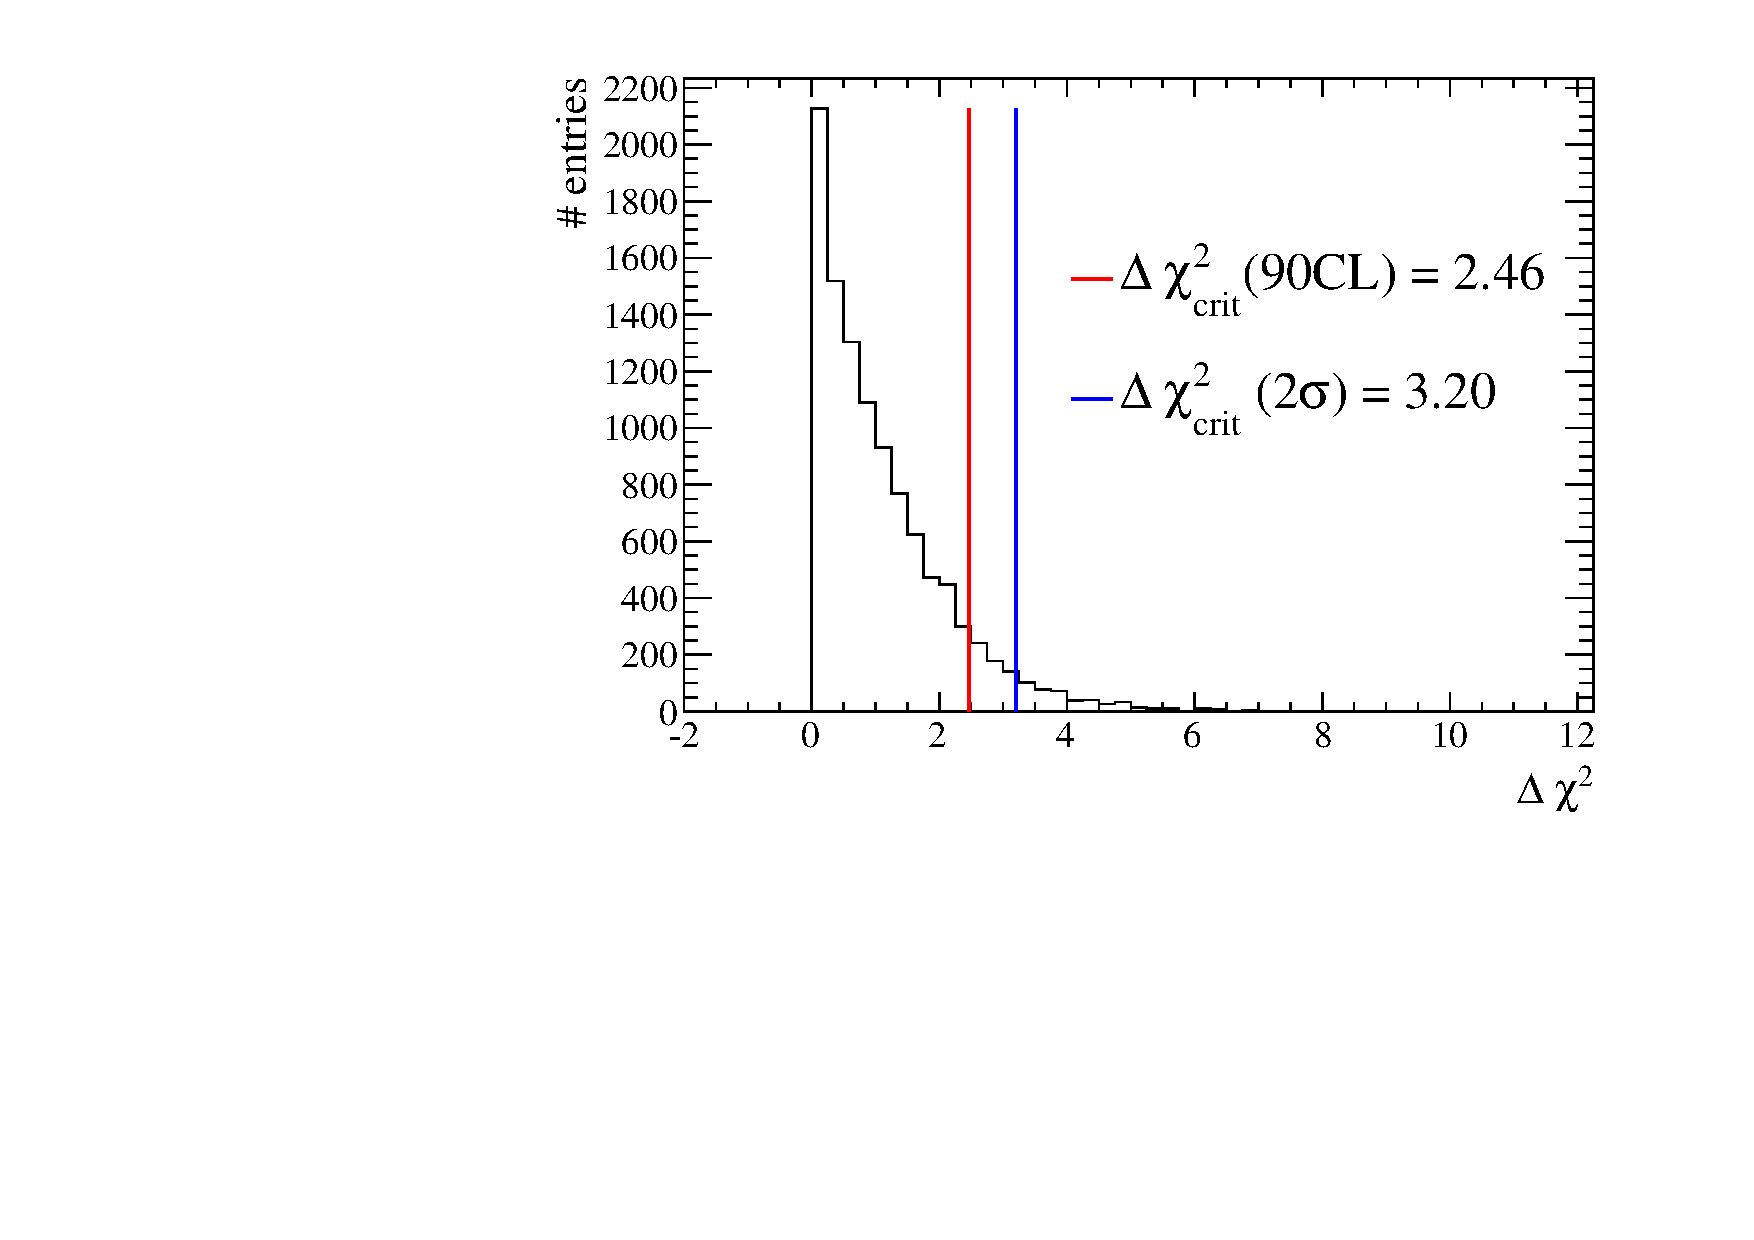
\includegraphics[width=0.9\textwidth]{./joint_plots/coverage_fc/coverage/deltachisq_glob_deltacp_0_1D_normal.pdf}
\caption{$\Delta \chi^2$ distribution.
$\delta_{CP}^{true} = 0$.}
\end{subfigure}
\begin{subfigure}[b]{0.49\textwidth}
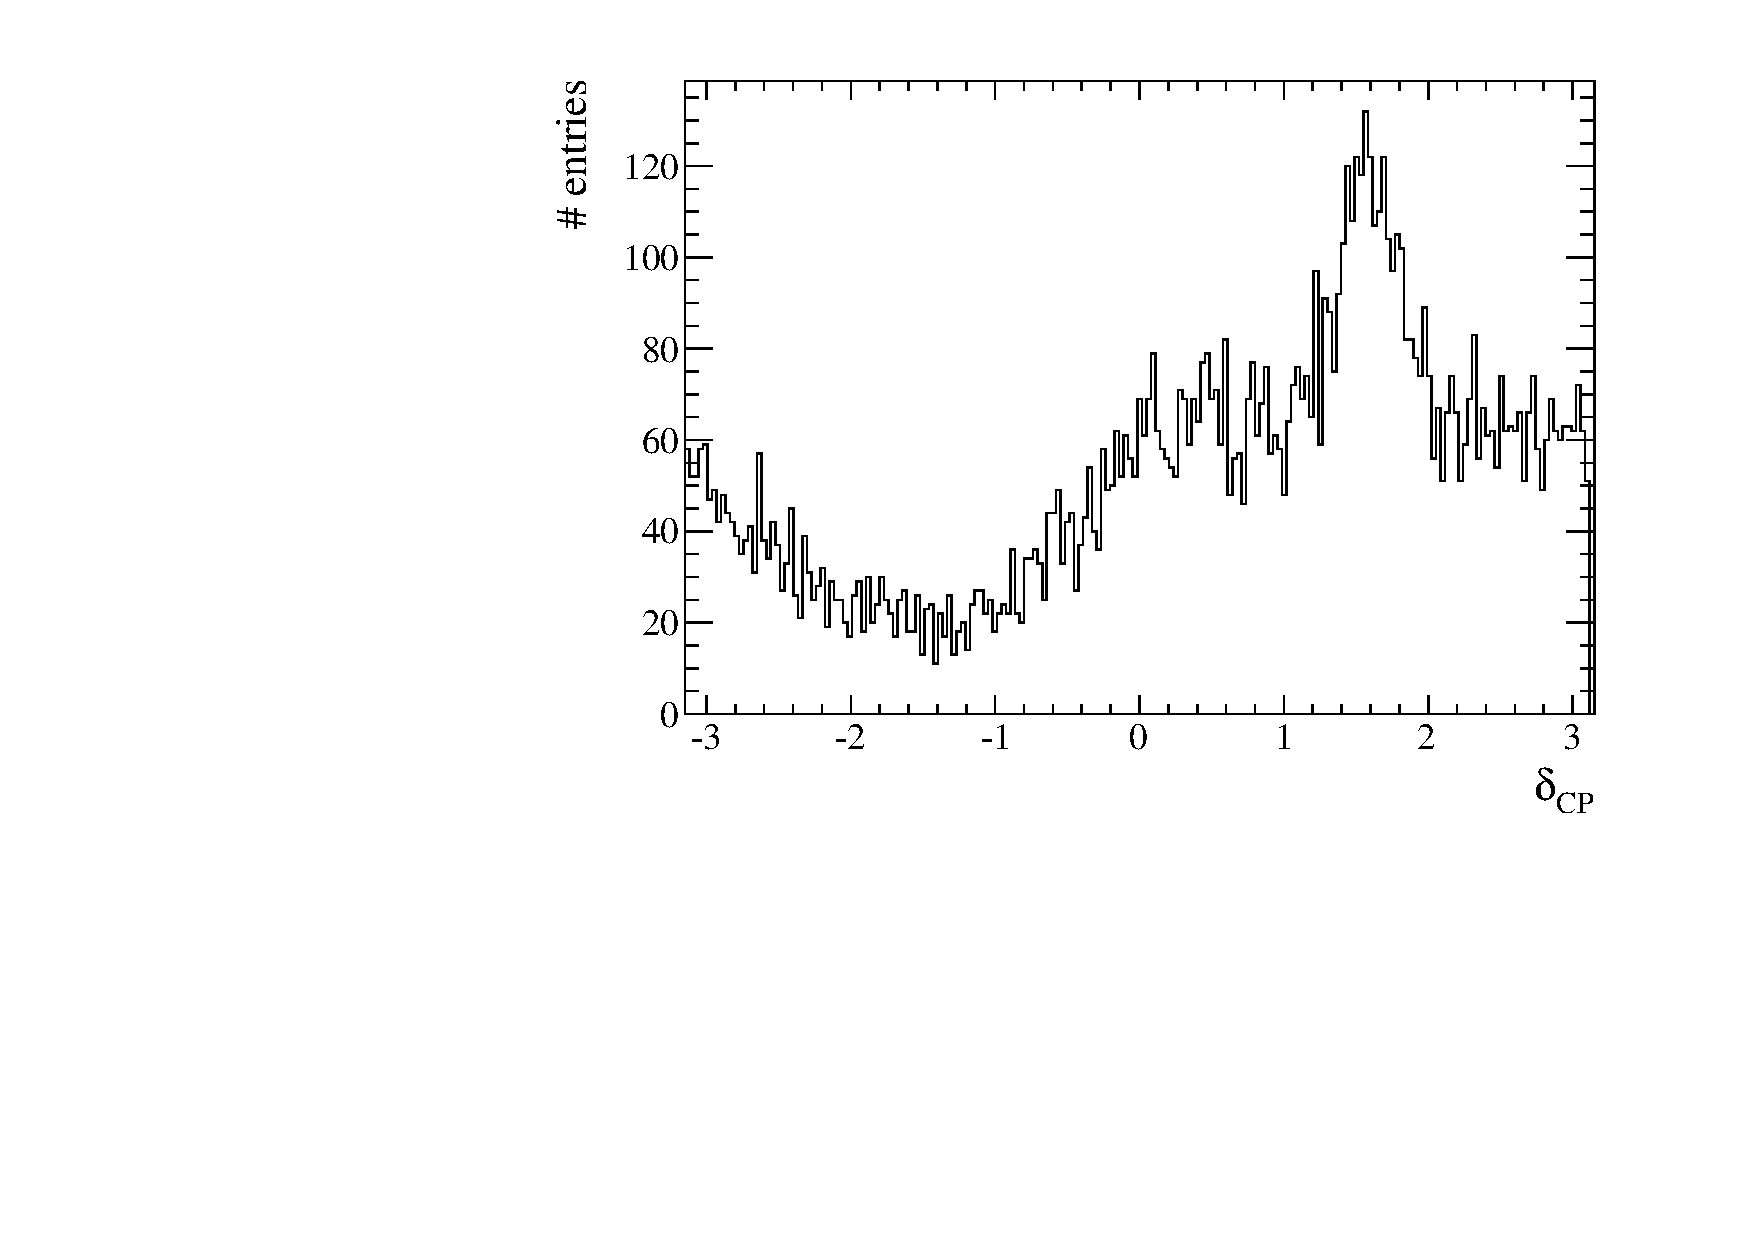
\includegraphics[width=0.9\textwidth]{./joint_plots/coverage_fc/coverage/cbestfit_deltacp_1p571_1D_normal.pdf}
\caption{Best-fit distribution of $\delta_{CP}$. $\delta_{CP}^{true} = +\pi/2$.}
\end{subfigure}
\begin{subfigure}[b]{0.49\textwidth}
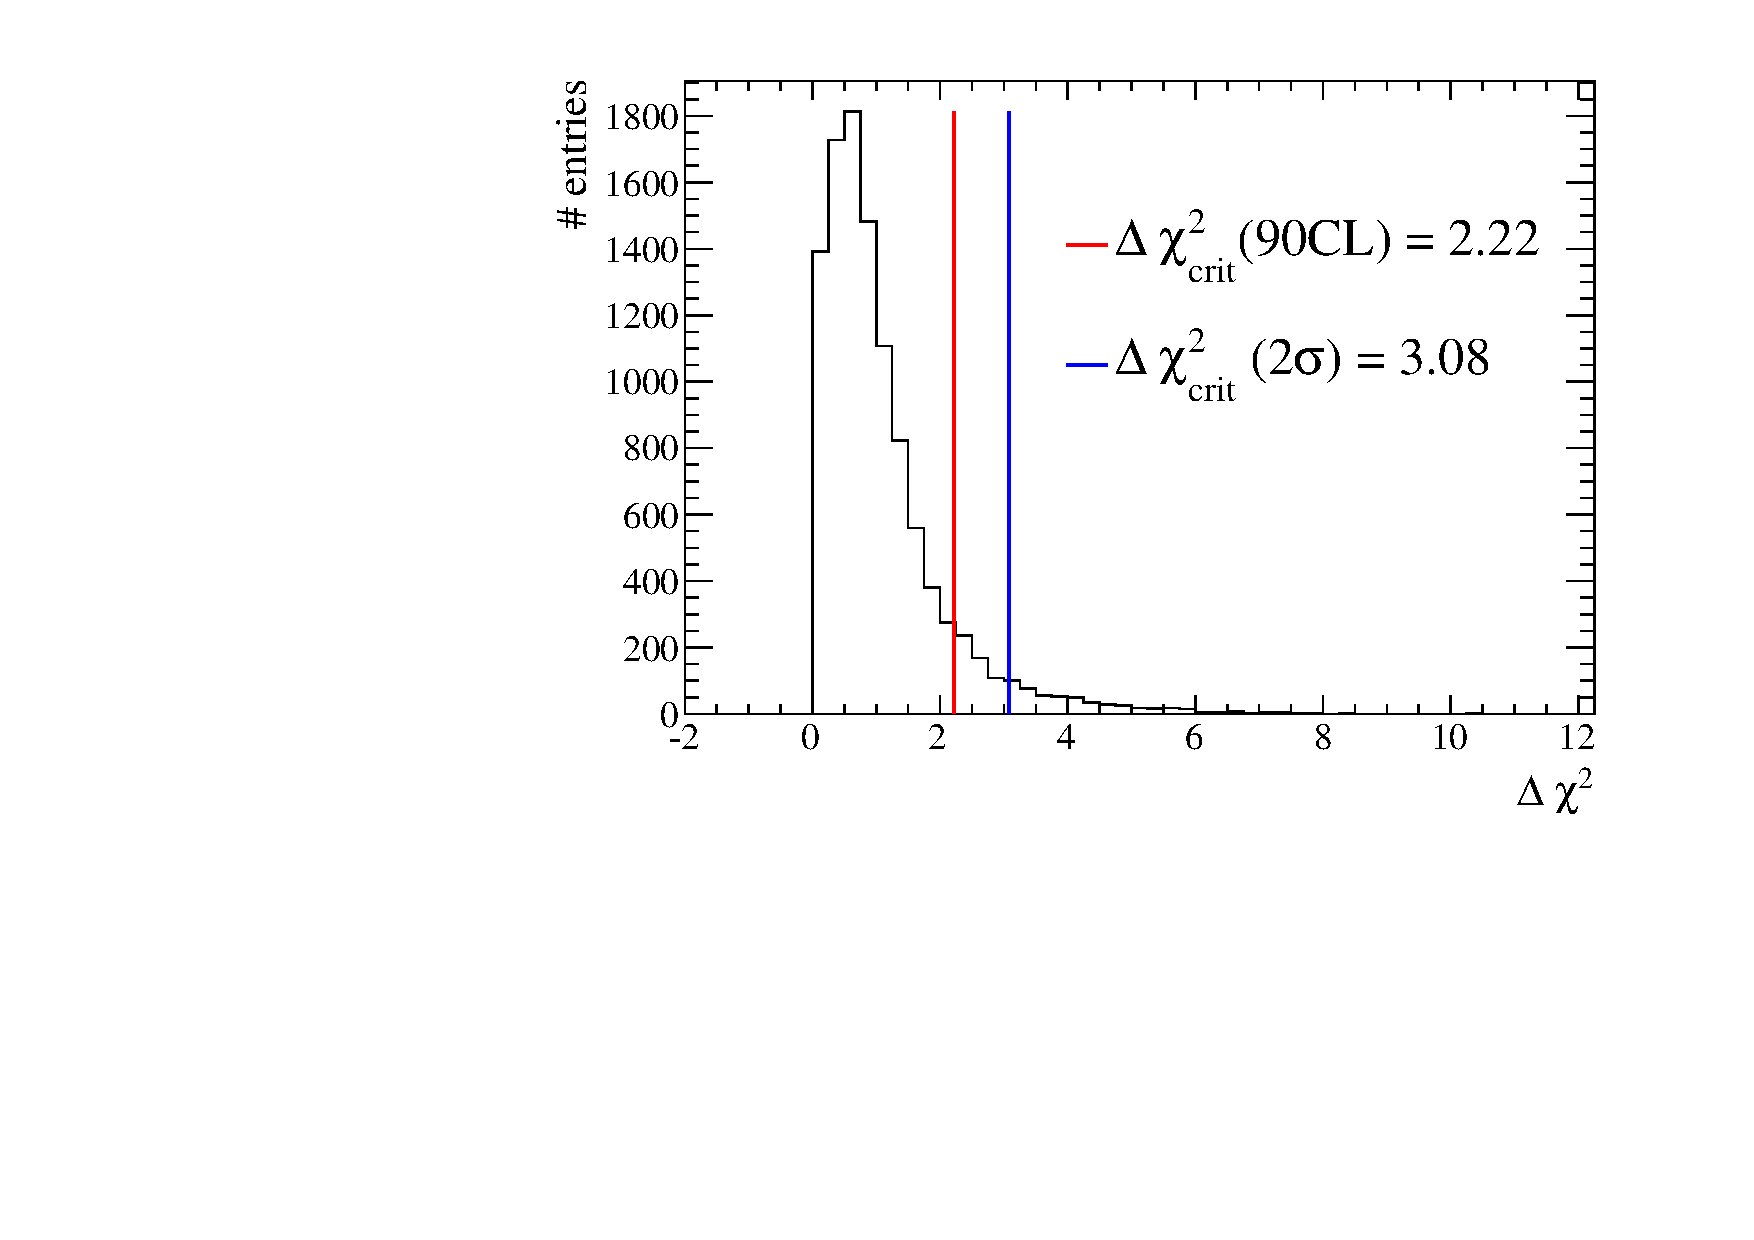
\includegraphics[width=0.9\textwidth]{./joint_plots/coverage_fc/coverage/deltachisq_glob_deltacp_1p571_1D_normal.pdf}
\caption{$\Delta \chi^2$ distribution.
$\delta_{CP}^{true} = +\pi/2$.}
\end{subfigure}
\caption {
Distributions of best-fit $\delta_{CP}$ (left) and $\Delta \chi^2$ (right).  
$10k$ toy experiments are performed
with true values of $\delta_{CP} = -\pi/2, 0, +\pi/2$, 
assuming normal hierarchy and applying the reactor constraint.
Both the mass hierarchy and $\delta_{CP}$ are profiled in the fit.
All the other oscillation parameters are marginalised.
The statistics corresponds to the Run 1-6 data set.
}
\label{fig:dchisq_bestfit_dcp}
\end{figure*}



\begin{table}
\center
\begin{tabular}{| c | c | c |}
\hline
 \multicolumn{3}{| c |}{\bf Gaussian approximation}  \\
\hline
{\bf CL} 			& \multicolumn{2}{c |}{\bf Critical value}  \\
\hline
\multicolumn{1}{| c |}{$1\sigma$}	& \multicolumn{2}{| c |}{1}  \\ \hline
\multicolumn{1}{| c |}{90\%}	& \multicolumn{2}{| c |}{2.71}  	\\ \hline
\multicolumn{1}{| c |}{$2\sigma$}	& \multicolumn{2}{| c |}{4}  \\ \hline
\hline
\multicolumn{3}{| c | }{{\bf Feldman-Cousins:} $\delta^{true}_{CP} = -\pi/2$, $MH^{true} = \text{normal}$}  \\
\hline
{\bf CL} 				& {\bf Critical value} &{\bf Coverage}  \\
\hline
$1\sigma$				& $0.582$ 		& 0.779	\\ \hline	
90\%					& $2.094$ 		& 0.935	\\ \hline	
$2\sigma$				& $3.242$		& 0.972	\\ \hline	
\hline
\multicolumn{3}{| c | }{{\bf Feldman-Cousins:} $\delta^{true}_{CP} = 0$, $MH^{true} = \text{normal}$}  \\
\hline
{\bf CL}				& {\bf Critical value} &{\bf Coverage}  \\
\hline
$1\sigma$				& $1.334$ 		& 0.570	\\ \hline	
90\%					& $2.460$ 		& 0.923	\\ \hline	
$2\sigma$				& $3.198$ 		& 0.981	\\ \hline	
\hline
\multicolumn{3}{| c | }{{\bf Feldman-Cousins:} $\delta^{true}_{CP} = +\pi/2$, $MH^{true} = \text{normal}$}  \\
\hline
{\bf CL} 				& {\bf Critical value} &{\bf Coverage}  \\
\hline
$1\sigma$				& $1.178$ 		& 0.605	\\ \hline	
90\%					& $2.224$ 		& 0.938	\\ \hline	
$2\sigma$				& $3.080$ 		& 0.977	\\ \hline	
\end{tabular}
\caption{
The critical values of $\Delta \chi^2$ used to set the confidence intervals are shown
for both the gaussian approximation (i.e. constant $\Delta \chi^2$) as
well as the ones obtained with the Feldman-Cousins method.
10k toy experiments were used for each true point of $\delta_{CP}$.
Furthermore the coverage, defined by \cref{eq:coverage},
provided by the gaussian approximation for different true values $\delta_{CP}$ is shown.
The true mass hierarchy is set to normal.
The collected statistic corresponds to the Run 1-6 data set one.
%The errors on the critical values are computed using \cref{eq:def_crit_val_error}
}             
\label{tab:critval_0_pmhalfpi}                                                                                                                                                                             
\end{table}

The constant $\Delta \chi^2$ method does not give the proper coverage when the 
parameter of interest is not gaussian distributed and when the relation with the likelihood is not linear.
Another reason why the correct coverage could not be assured by the constant $\Delta \chi^2$
method is the presence of physical boundaries. 
$\delta_{CP}$ is continuous because it is periodic, however it shows up physical boundaries at $\pm \pi/2$,
since they correspond to the values that maximize or minimize the number of events in the
$e$-like samples. 
In general the gaussian approximation gives over-coverage for all the listed confidence intervals,
except for $1\sigma$ CL of $\delta^{true}_{CP} = +\pi/2$ and 0 with $MH^{true} = \text{normal}$.
\newline

% deltaCP=+pi/2 and Normal Hierarchy
This can be understood by analyzing the best-fit result of 10k toy experiments 
with $\delta^{true}_{CP} = +\pi/2$ and normal hierarchy.
In this case the constant $\Delta \chi^2$ method gives under-coverage for $1\sigma$ CL
(the constant critical value is larger than the one computed with Feldman-Cousins)
but over-coverage for 90\% and $2\sigma$ CL 
(the constant critical value is smaller than the one computed with Feldman-Cousins).
In general a critical value estimated with Feldman-Cousins is larger (smaller)
when the $\Delta \chi^2$ distribution is wider (tighter),
that is favored when the best-fit parameter values are different from (same as) the true values (see \cref{eq:fc_dcp_mh}). 
Wider $\Delta \chi^2$ distributions are due to degeneracy with other parameters, in this case the mass hierarchy.
Indeed in \cref{fig:mass_hierarchy_MC_shift} it is shown that the inverted hierarchy increases the expected
number of events in antineutrino mode $e$-like sample and reduces it in neutrino mode $e$-like sample,
similarly to the effect of $\delta_{CP} = +\pi/2$ (see \cref{tab:eventrate_dcp_mh}).
On average the best-fit mass hierarchy is chosen to be inverted $\sim 70\%$ of the times
and the best-fit distribution of $\delta_{CP}$ is peaked at $+\pi/2$.
This is due to asymmetric fluctuations: upward statistical fluctuations in the antineutrino mode $e$-like sample
and downward statistical fluctuations in the neutrino mode $e$-like sample.
One would expect the mass hierarchy best-fit to be inverted $\sim 50\%$ of the times.
However it should be considered that $\delta_{CP} = +\pi/2$, the true point, behaves as a physical boundary.
So about half of the extreme asymmetric fluctuations would need more events in antineutrino mode
and less in antineutrino mode than what $\delta_{CP} = +\pi/2$ can provide.
For this reason the only possible way to fit these fluctuations is to choose inverted hierarchy,
which has an effect similar to $\delta_{CP} = +\pi/2$.
Another way to see it is by looking the $\Delta \chi^2$ distribution corresponding to 
fits where the best-fit mass hierarchy is normal, shown in \cref{fig:bf_dcp_bfNH}.
This fits correspond to opposite asymmetric fluctuations:
downward statistical fluctuation in the antineutrino mode $e$-like sample and
upward statistical fluctuation in the neutrino mode $e$-like sample. 
If the best-fit mass hierarchy is normal, the $\Delta \chi^2$ distribution of $\delta_{CP}$ is quite flat,
which means that to fit this asymmetric fluctuation the $\delta_{CP}$ parameter is enough,
because the other physical boundary is at $-\pi/2$ which is far from the true point. 

\begin{figure*}[htb]
\center
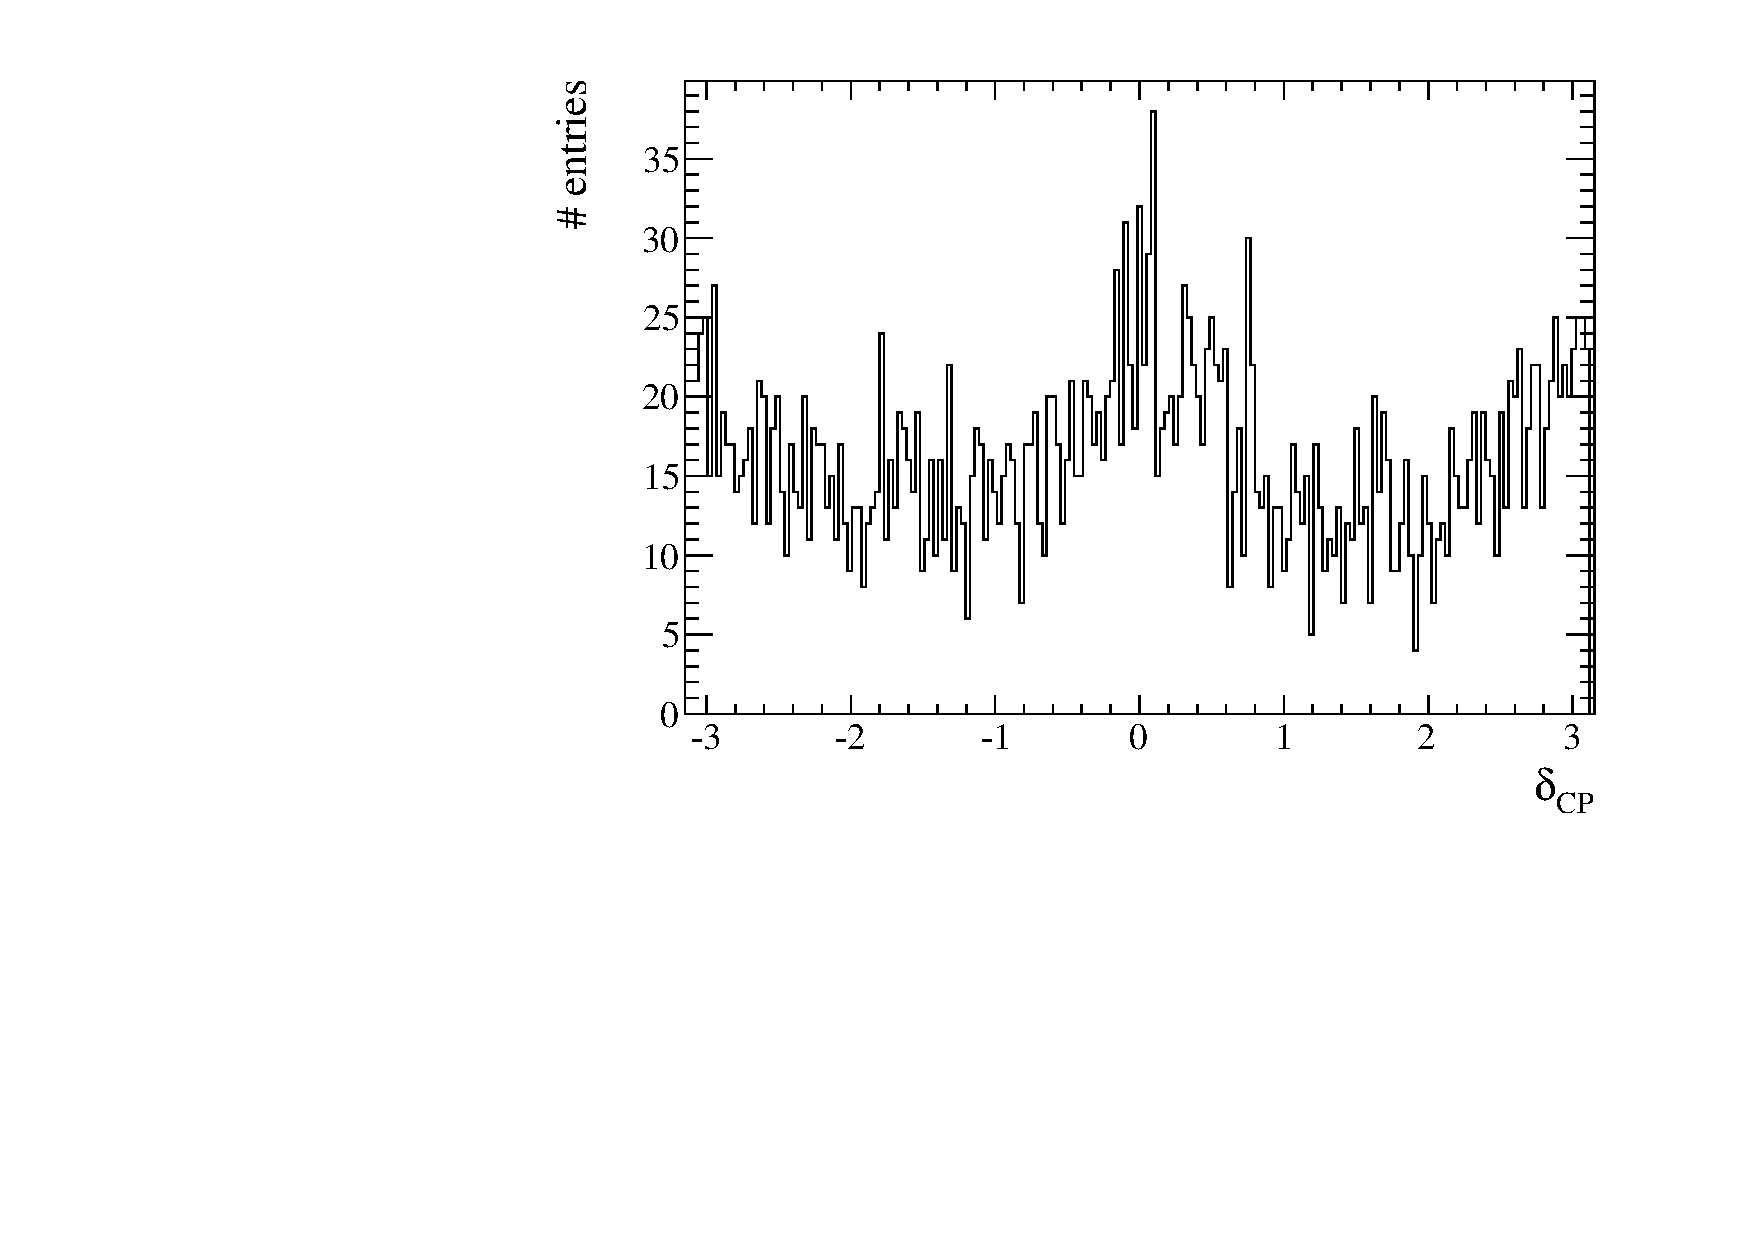
\includegraphics[width=0.49\textwidth]{./joint_plots/coverage_fc/coverage/p_pi_over_2/bf_dcp_bfNH.pdf}
\caption{Best-fit $\delta_{CP}$ distribution for fits where the best-fit mass hierarchy is normal.
The true values correspond to $\delta_{CP} = +\pi/2$ and normal hierarchy.}
\label{fig:bf_dcp_bfNH}
\end{figure*}

The under-coverage at 68\% CL, i.e. estimated critical value is larger than 1, is due 
to the degeneracy between $\delta_{CP}$ and mass hierarchy 
as well as the fact that the true point
is at the physical boundary.
The true point corresponds to values of mass hierarchy (normal) and $\delta_{CP}$ ($+\pi/2$) that 
have opposite effects and balance between each other.
So if $\delta_{CP}^{bf} = +\pi/2$, 
in order to compensate the physical boundary in $\delta_{CP}$,
the best-fit mass hierarchy is inverted, 
which is different from the true one.
Consequently \cref{eq:fc_dcp_mh} will not have $\Delta \chi^2 \sim 0$ values.
On the other hand the opposite happens when the true point is  $\delta_{CP}^{true} = -\pi/2$ and normal hierarchy.
Indeed in this case there is over-coverage, i.e. the critical value is smaller.
This happens because $\delta_{CP}^{true}$ is at a physical boundary but the true mass hierarchy 
has the same effect on the spectra. So extreme asymmetric statistical fluctuations cannot
be accomodated by neither $\delta_{CP}$ nor mass hierarchy, which best-fit values will correspond
most of the time to the true point, as shown in \cref{fig:bf_MH_nh_dcp_ppi2}.
For this reason \cref{eq:fc_dcp_mh} will give more values of $\Delta \chi^2$ close to 0,
producing a tighter distribution and consequently smaller critical values, as shown in \cref{fig:dchisq_bestfit_dcp}.

In order to test confidence intervals for higher significance the tail of the $\Delta \chi^2$ distribution is more important. 
In \cref{fig:bf_MH_nh_dcp_ppi2} the best-fit mass hierarchy and $\delta_{CP}$ distributions
are shown only for those toy experiments which best-fit $\Delta \chi^2$ is larger than 2.
This toy experiments correspond to the following asymmetric fluctuations of the data 
(upward for neutrino mode $e$-like sample
and downward for antineutrino $e$-like sample)
that prefer values of $\delta_{CP} \sim -\pi/2$ and normal hierarchy.
Since normal hierarchy corresponds to the true point 
and there is no other possible value of mass hierarchy that can better fit the statistical fluctuation,
\cref{eq:fc_dcp_mh} becomes relatively small enough to produce a tighter distribution
in the range of large $\Delta \chi^2$. 
\newline

% deltaCP=+pi/2 and Normal Hierarchy
Another proof of this behavior can be given by looking to \cref{fig:bf_MH_nh_dcp_mpi2},
that shows the best-fit mass hierarchy obtained with 10k toy experiments
with $\delta_{CP}^{true} = -\pi/2$ and normal hierarchy.
In this case also for the $1\sigma$ CL the constant $\Delta \chi^2$ method gives over-coverage,
because the $\Delta \chi^2$ distribution is tighter.
The reason is that $\delta_{CP} = -\pi/2$ is degenerate with normal hierarchy 
(they have similar effects on the $e$-like spectra), which is the true mass hierarchy,
and there is no other possible value of mass hierarchy able to fit extreme fluctuations.
For this reason \cref{eq:fc_dcp_mh} becomes relatively tight in the tail.
\newline

\begin{figure*}[htb]
\center
\begin{subfigure}[b]{0.49\textwidth}
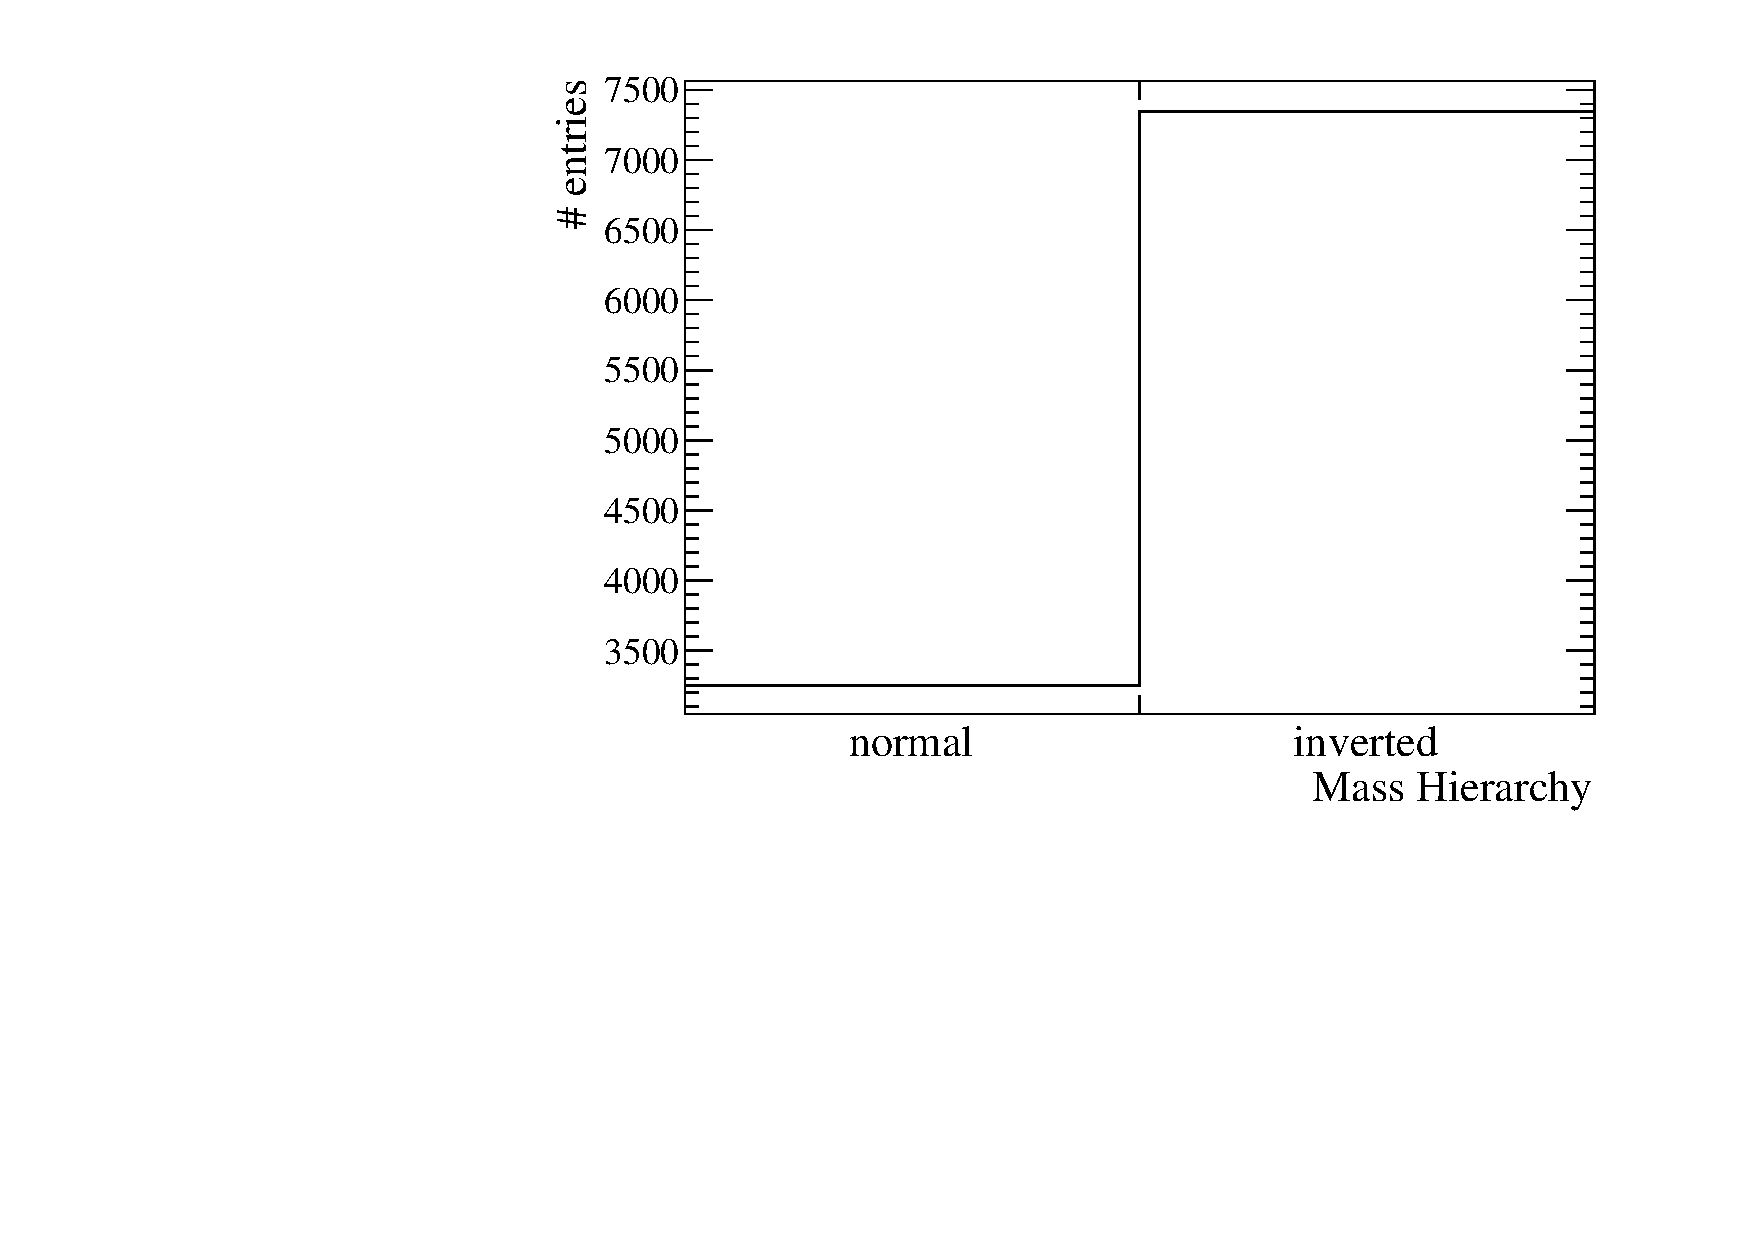
\includegraphics[width=0.9\textwidth]{./joint_plots/coverage_fc/coverage/cbestfit_MH_deltacp_1p571_1D_normal.pdf}
\caption{Best-fit mass hierarchy distribution.}
\end{subfigure} 
\begin{subfigure}[b]{0.49\textwidth}
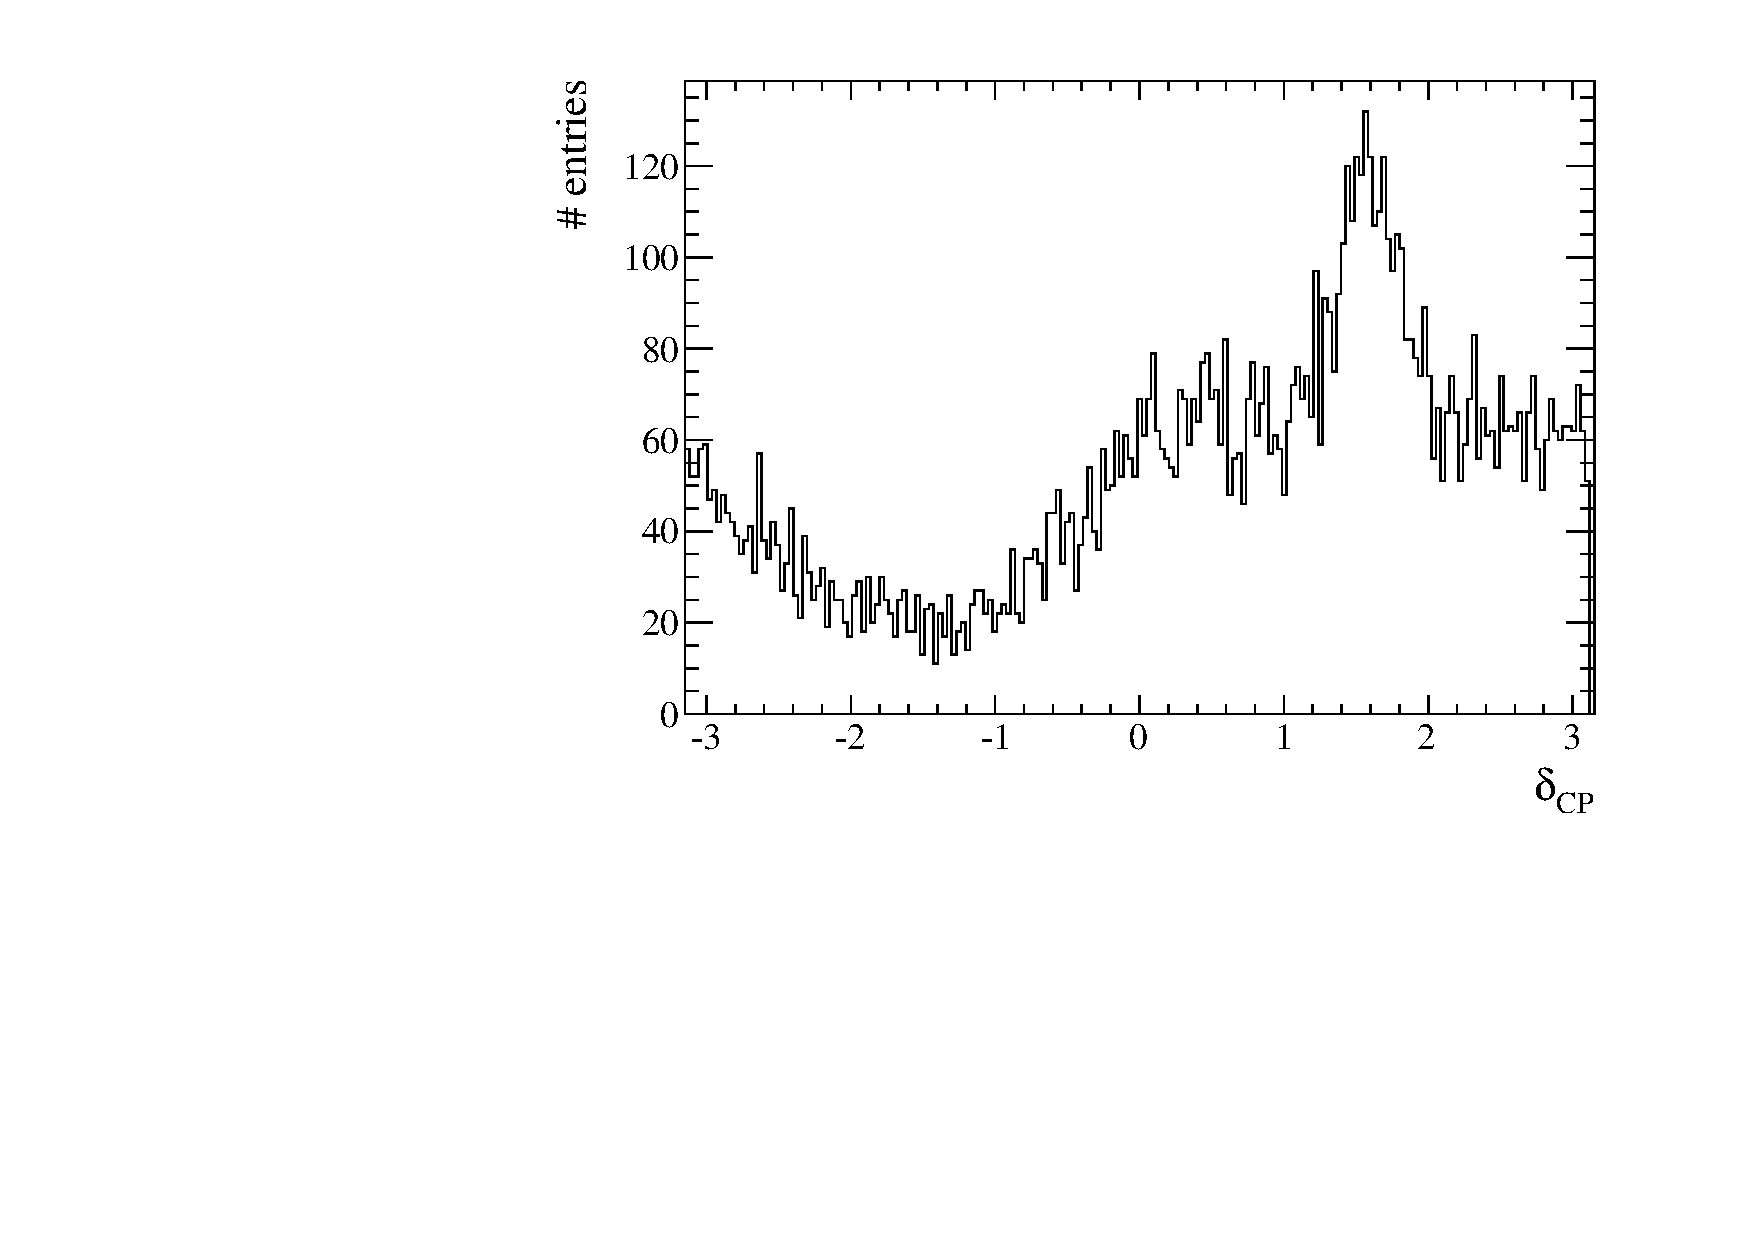
\includegraphics[width=0.9\textwidth]{./joint_plots/coverage_fc/coverage/cbestfit_deltacp_1p571_1D_normal.pdf}
\caption{Best-fit distribution of $\delta_{CP}$.}
\end{subfigure} \\
\begin{subfigure}[b]{0.49\textwidth}
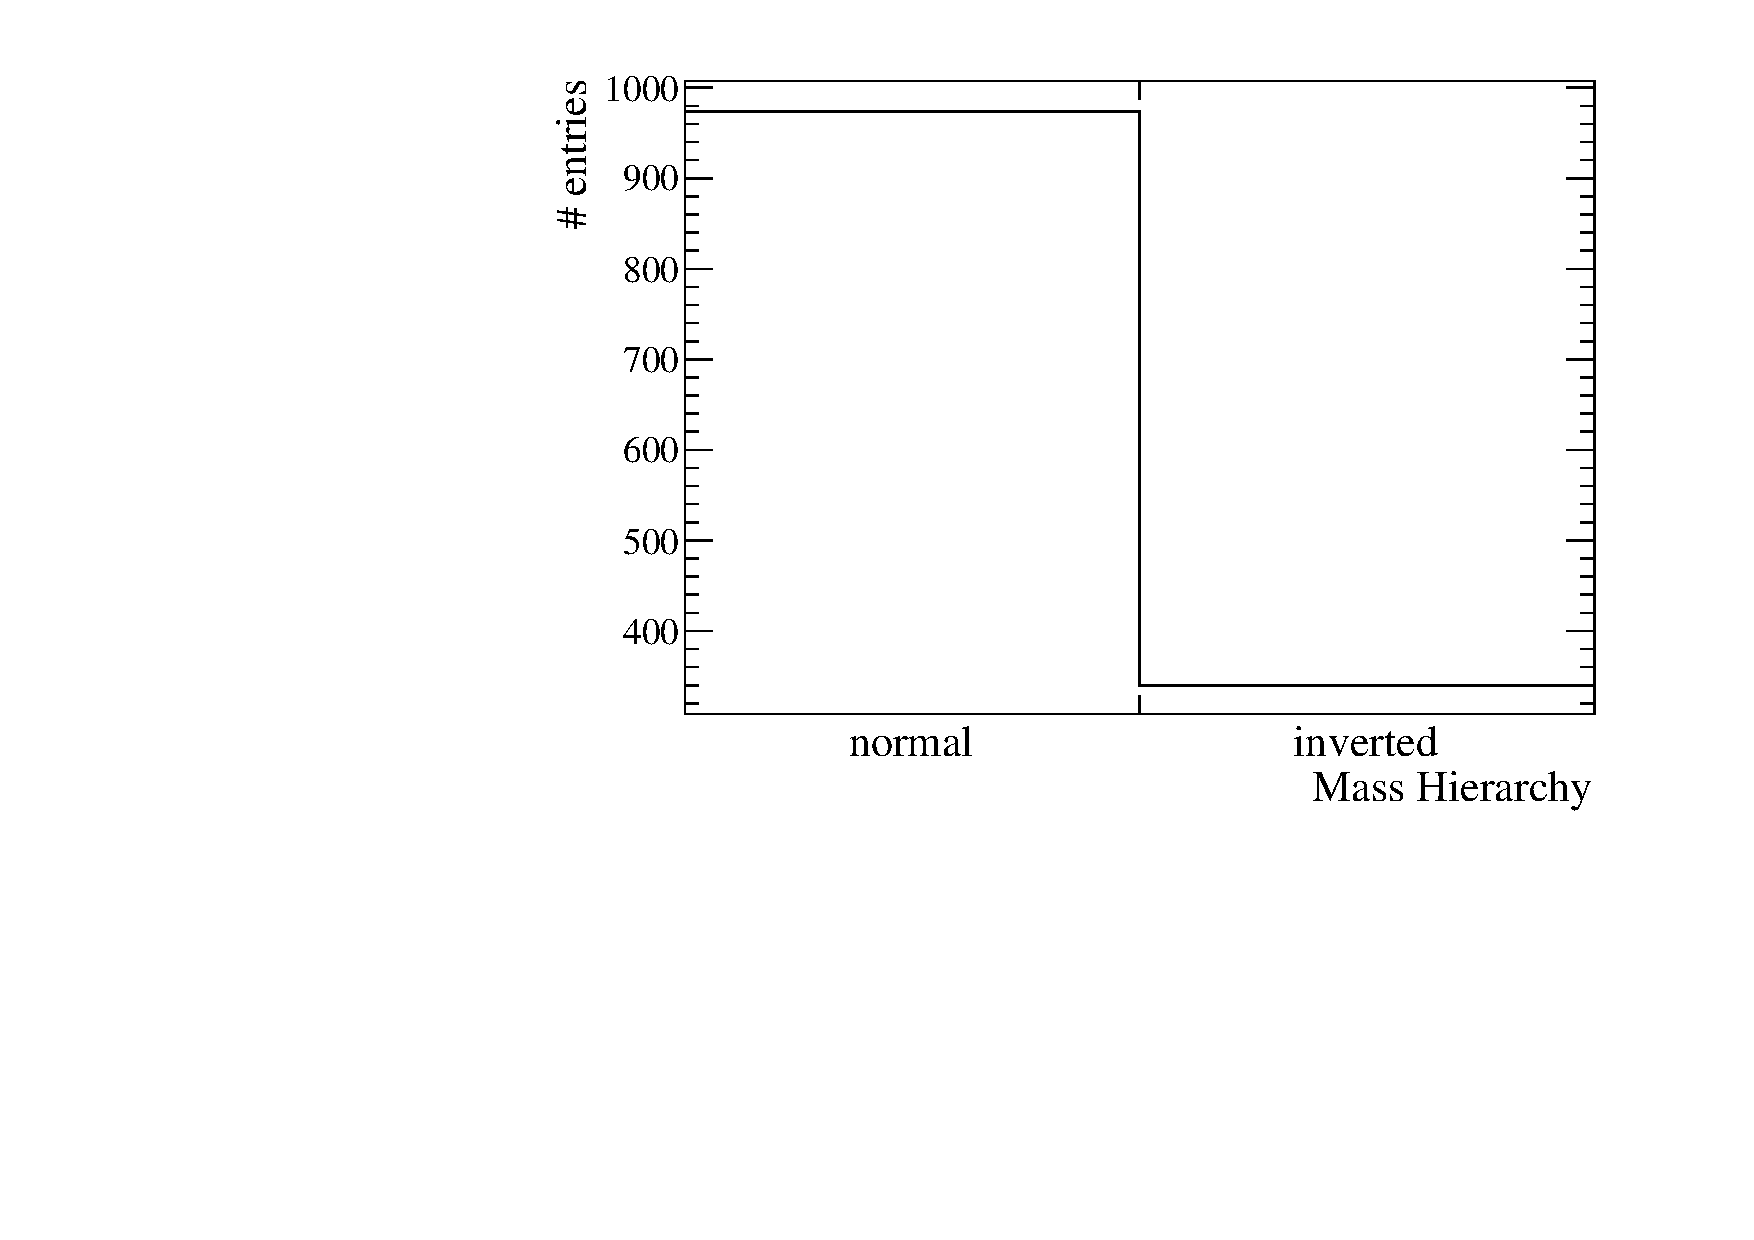
\includegraphics[width=0.9\textwidth]{./joint_plots/coverage_fc/coverage/cbestfit_MH_deltacp_1p571_1D_normal_deltachisq_below_2.pdf}
\caption{Best-fit mass hierarchy distribution. 
Only fits with best-fit $\Delta \chi^2 > 2$ are selected.}
\end{subfigure}
\begin{subfigure}[b]{0.49\textwidth}
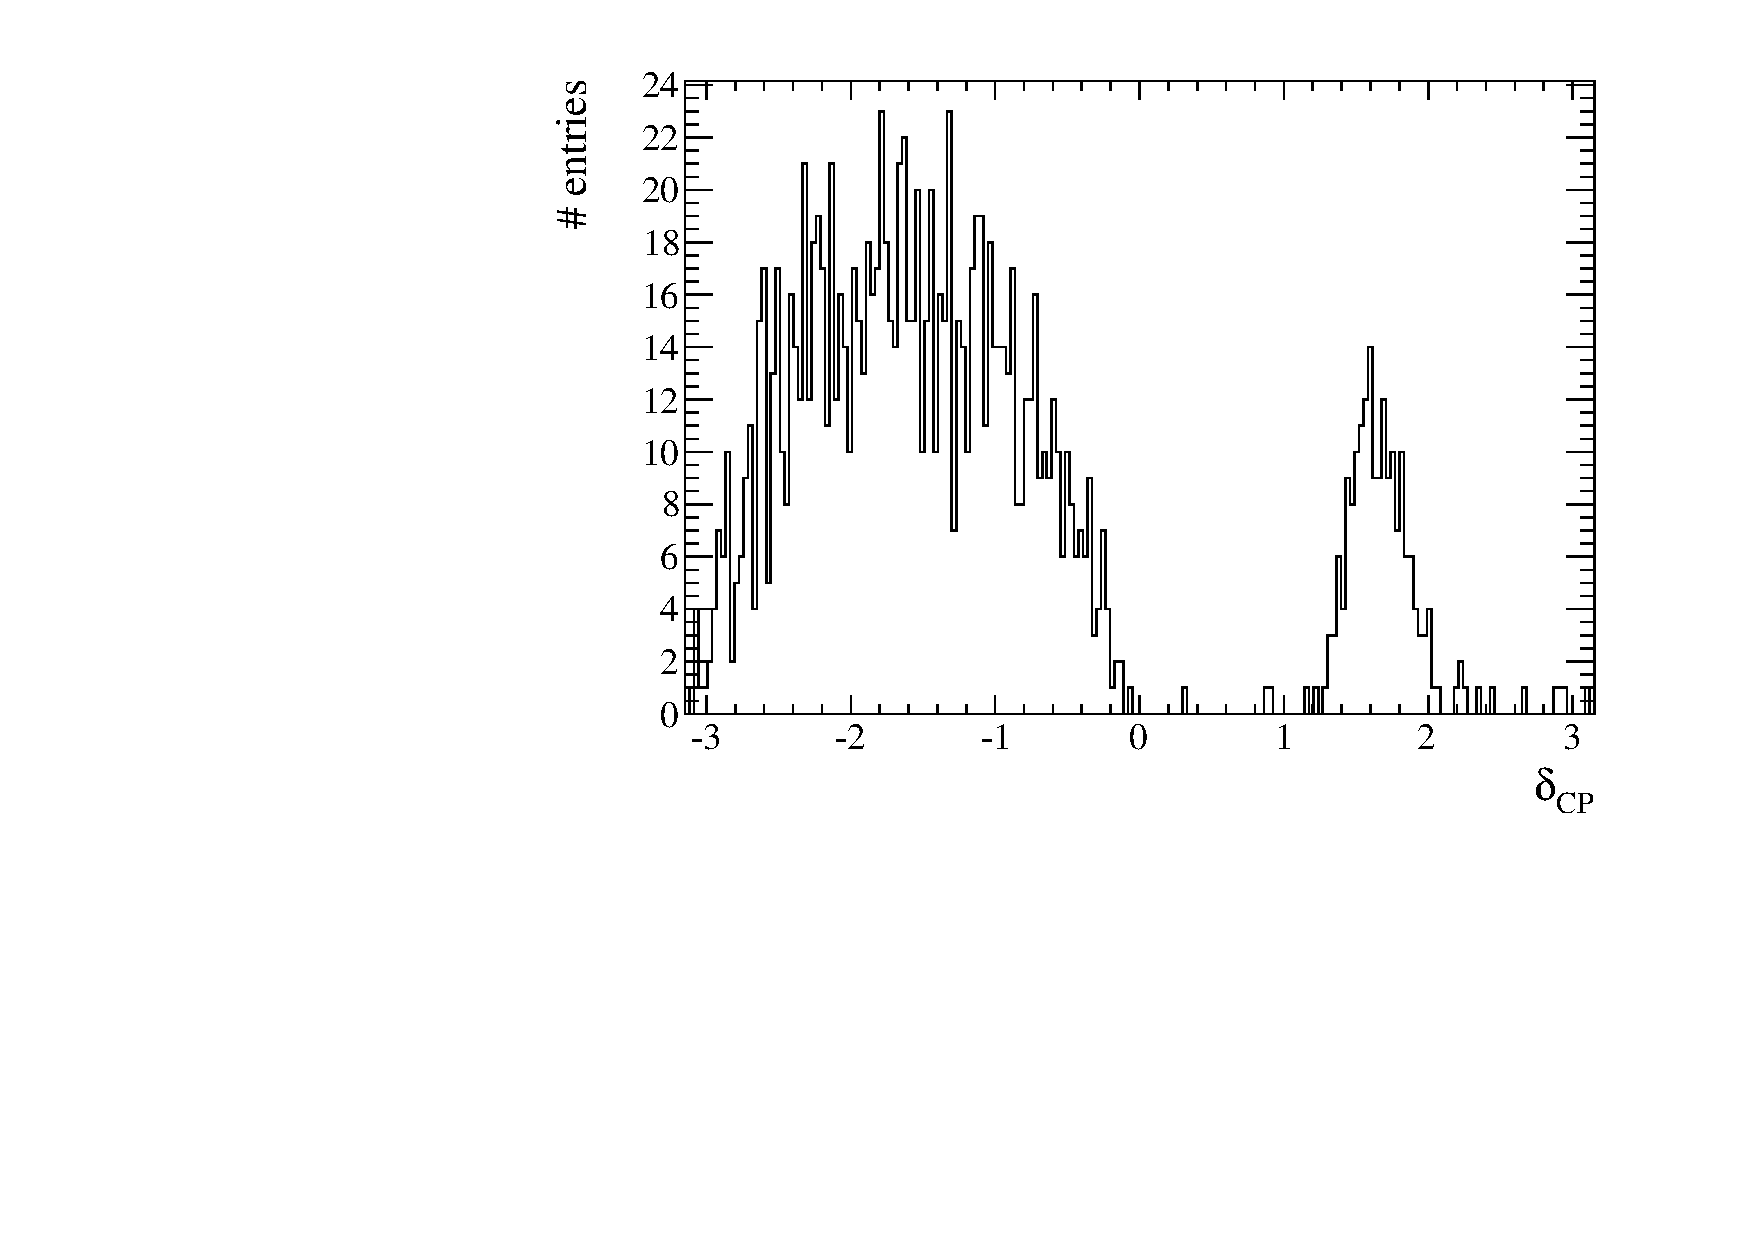
\includegraphics[width=0.9\textwidth]{./joint_plots/coverage_fc/coverage/cbestfit_deltacp_1p571_1D_normal_deltachisq_below_2.pdf}
\caption{Best-fit $\delta_{CP}$ distribution. 
Only fits with best-fit $\Delta \chi^2 > 2$ are selected.}
\end{subfigure}\\
\caption {
Best-fit distribution of mass hierarchy and $\delta_{CP}$ from the simultaneous fit of $\delta_{CP}$ and mass hierarchy.
$10k$ toy experiments are produced with $\delta^{true}_{CP} = +\pi/2$ and normal hierarchy.
}
\label{fig:bf_MH_nh_dcp_ppi2}
\end{figure*}

\begin{figure*}[htb]
\center
\begin{subfigure}[b]{0.49\textwidth}
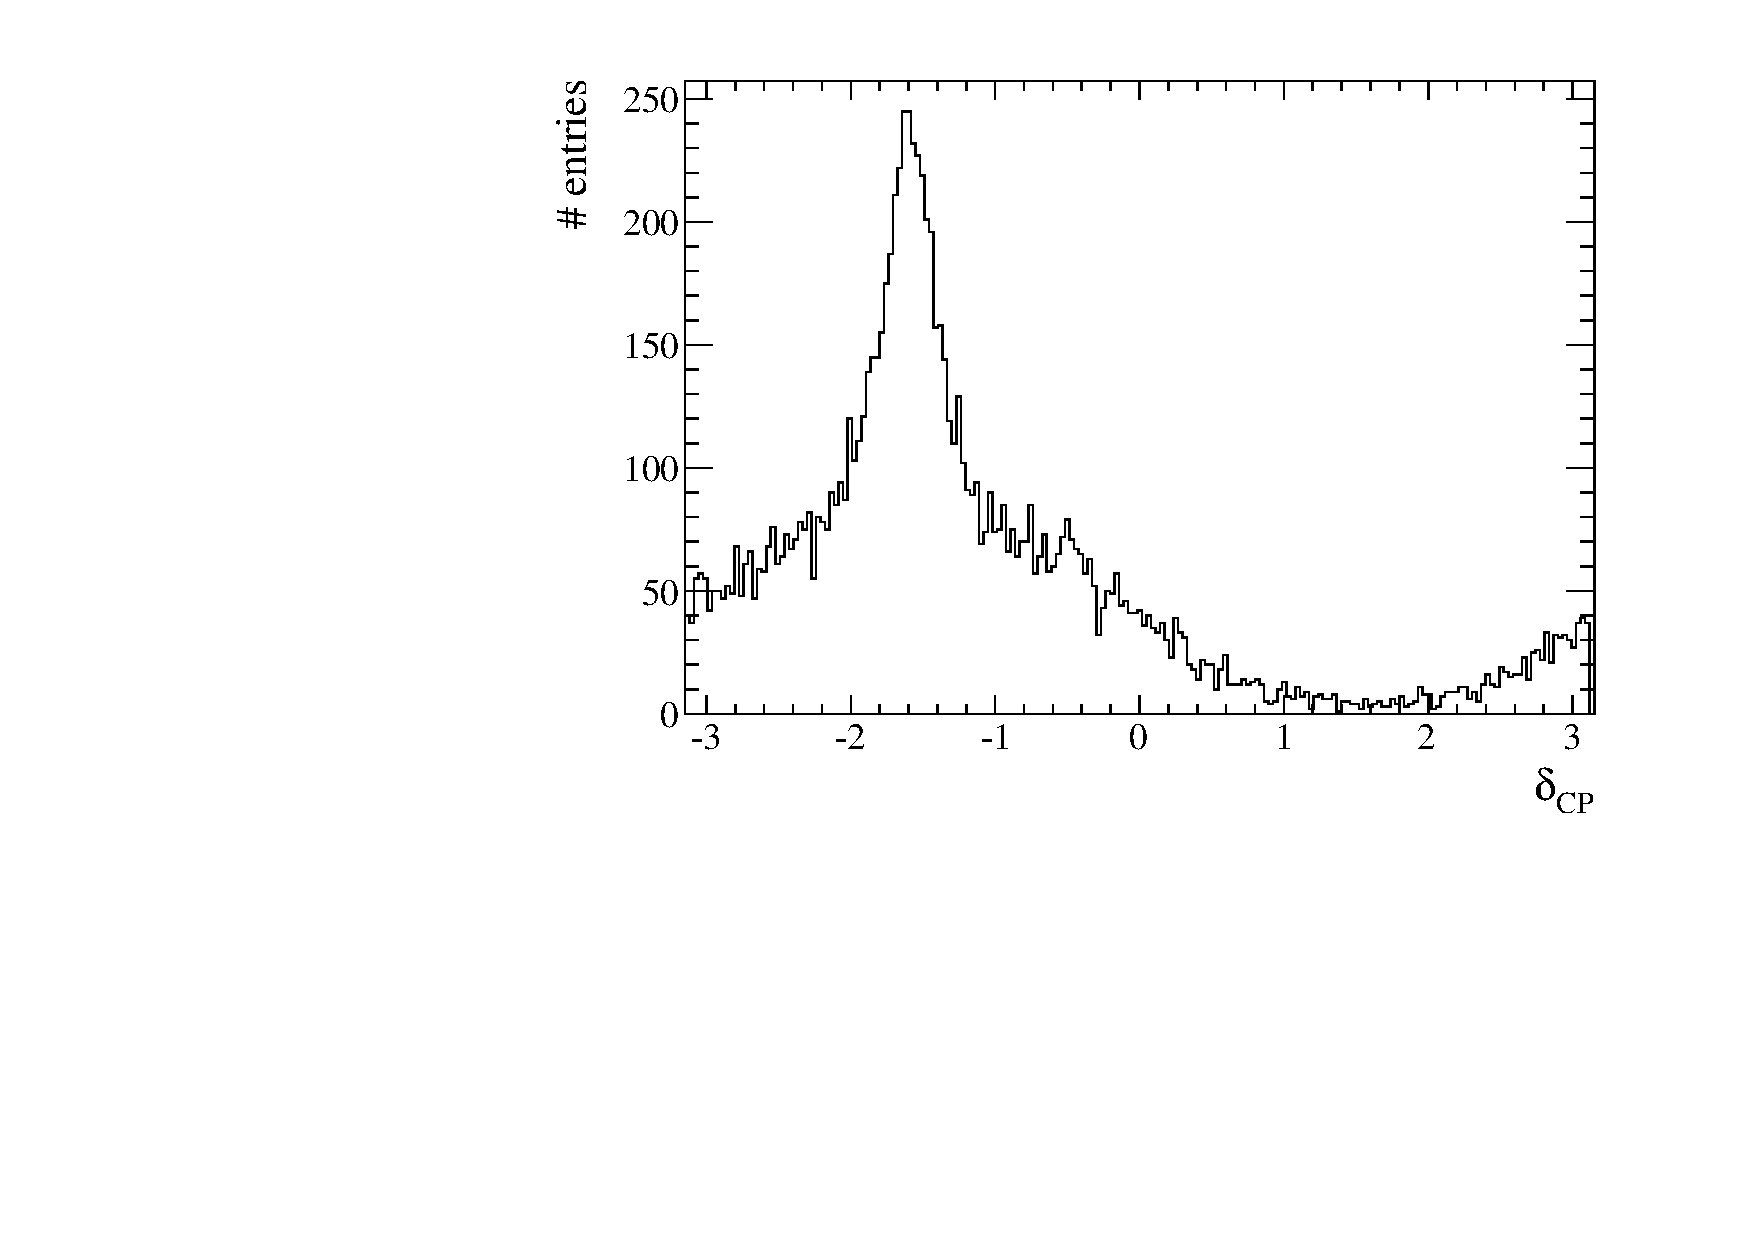
\includegraphics[width=0.9\textwidth]{./joint_plots/coverage_fc/coverage/cbestfit_deltacp_-1p571_1D_normal.pdf}
\caption{Best-fit distribution of $\delta_{CP}$.}
\end{subfigure}
\begin{subfigure}[b]{0.49\textwidth}
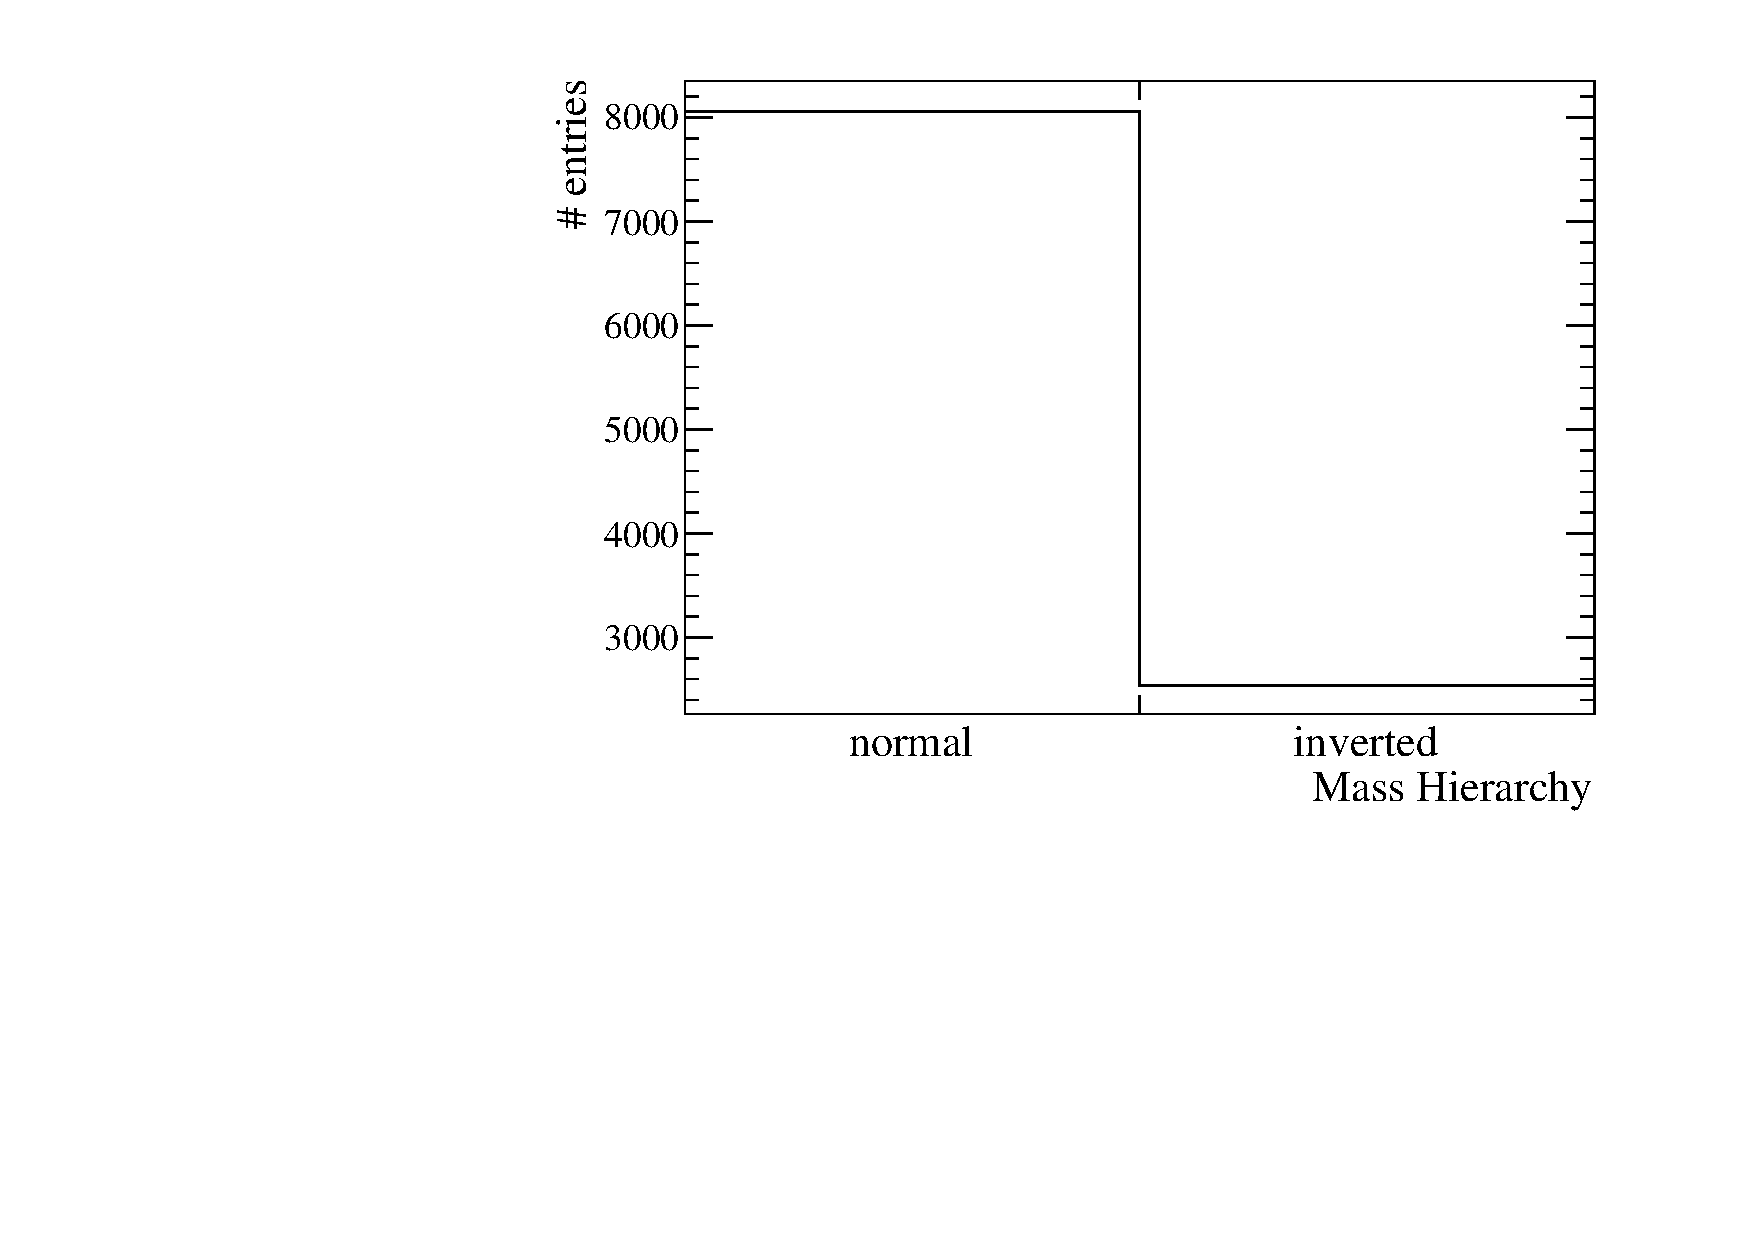
\includegraphics[width=0.9\textwidth]{./joint_plots/coverage_fc/coverage/cbestfit_MH_deltacp_m1p571_1D_normal.pdf}
\caption{Best-fit distribution of mass hierarchy.}
\end{subfigure}
\caption {
Best-fit distribution of mass hierarchy from the simultaneous fit of $\delta_{CP}$ and mass hierarchy.
$10k$ toy experiments are produced with $\delta^{true}_{CP} = -\pi/2$ and normal hierarchy.
}
\label{fig:bf_MH_nh_dcp_mpi2}
\end{figure*}


% deltaCP=0 and Normal Hierarchy
From the best-fit distributions of $\delta_{CP}$ we can see that the current statistic is still not enough
for a precise measurement of $\delta_{CP}$. 
However if $\delta^{true}_{CP} = \pm \pi/2$ the best-fit distribution shows a peak around the true value.
For $\delta^{true}_{CP} = 0$ the fit prefers values smaller than 0,
though the true mass hierarchy is normal, it is chosen as best-fit only about 54\% of the times.
This is, again, due to the degeneracy between the mass hierarchy and $\delta_{CP}$.
The normal hierarchy (true value) is not enough to fit extreme upward fluctuations in neutrino mode and 
downward fluctuations in antineutrino mode $e$-like sample, since the mass hierarchy is in a discrete boundary.
So values of $\delta_{CP} \sim -\pi/2$ are favored in order to balance it.
Furthermore in these fits the normal hierarchy is preferred with respect to inverted hierarchy
about the 65\% of the times.
Indeed if we only look to the fits where the normal hierarchy is preferred, i.e. the true value, 
the best-fit distribution of $\delta_{CP}$ is symmetrically distributed around 0. 
as shown in \cref{fig:bf_dcp_fix_nh}.

\begin{figure*}[htb]
\center
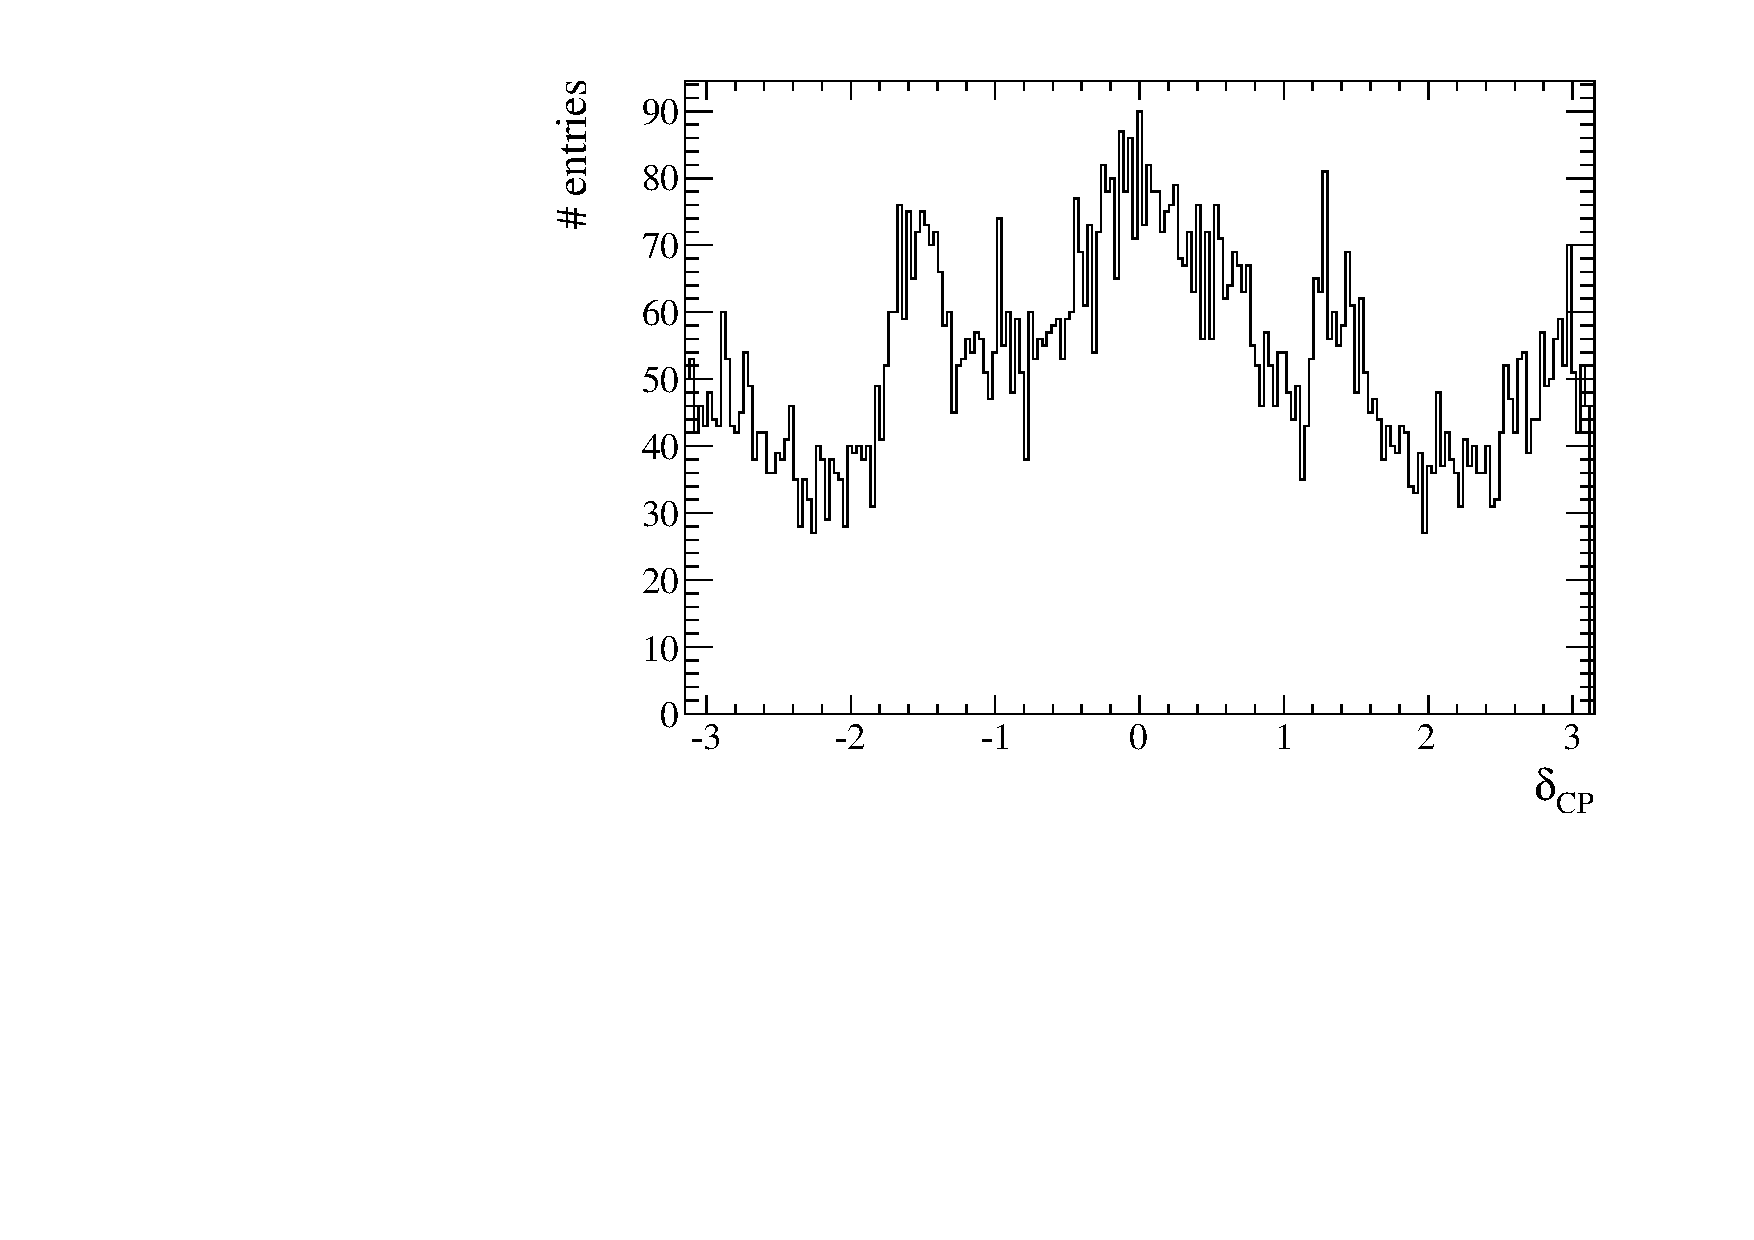
\includegraphics[width=0.5\textwidth]{./joint_plots/coverage_fc/coverage/cbestfit_nh_deltacp_0_1D_normal.pdf}
\caption {
Best-fit distribution of $\delta_{CP}$ obtained by fixing the mass hierarchy to normal and not profiled.
$10k$ toy experiments are produced with $\delta^{true}_{CP} = 0$ and normal hierarchy.
}
\label{fig:bf_dcp_fix_nh}
\end{figure*}

%The $\Delta \chi^2$ distribution corresponding to $\delta^{true}_{CP} = -\pi/2$ shows a spike at 0.
%This comes from the intrinsic physical boundary present at $-\pi/2$, since 
%the $\sin \delta_{CP}$ term in the oscillation probability has a upper boundary at $\pm \pi/2$.
%Since the true mass hierarchy is normal and the $\delta^{true}_{CP} = -\pi/2$ 
%a downward fluctuation in the antineutrino $e$-like sample and a upward fluctuation
%in the neutrino mode $e$-like sample cannot be accomodated by changing the hierarchy to inverted,
%since it have an opposite effect, and further need to choose $- \pi / 2$ as best-fit value.
%A similar behavior is shown in the best-fit distribution of $\delta^{true}_{CP} = +\pi/2$,
%though the effect is smaller because 
%a downward fluctuation in the neutrino $e$-like sample and a upward fluctuation
%in the antineutrino $e$-like sample can be accomodated also by choosing the hierarchy as inverted,
%since it has a degenerate effect as $\delta_{CP} = +\pi/2$. 

In general most of the strange behaviors present in the best-fit and $\Delta \chi^2$ distributions
can be explained with a still low sensitivity to both $\delta_{CP}$ and mass hierarchy 
and the strong degeneracy between the two oscillation parameters.
   


\begin{table}
\center
\begin{tabular}{| c | c | c | c |}
\hline
				\multicolumn{4}{| c |}{\bf $e$-like neutrino mode}  \\
\hline
	 				& $\delta_{CP} = -\pi/2$ 	& $\delta_{CP}=0$ 	& $\delta_{CP}=+\pi/2$  \\
\hline
Normal Hierarchy		& 26.596				& 22.407			& 18.179 	\\ \hline	
Inverted Hierarchy		& 23.554 				& 19.704			& 15.891	\\ \hline	
\hline
				\multicolumn{4}{| c |}{\bf $e$-like antineutrino mode}  \\
\hline
	 				& $\delta_{CP} = -\pi/2$ 	& $\delta_{CP}=0$ 	& $\delta_{CP}=+\pi/2$  \\
\hline
Normal Hierarchy		& 3.219 				& 3.704			& 4.122 	\\ \hline	
Inverted Hierarchy		& 3.475				& 3.987			& 4.499	\\ \hline	
\end{tabular}
\caption{
Expected number of events for neutrino and antineutrino mode $e$-like sample
for different values of $\delta_{CP}$ and mass hierarchy.
}             
\label{tab:eventrate_dcp_mh}                                                                                                                                                                             
\end{table}


%
% Posterior predictive method
%

\subsection{Posterior predictive method for the choice of the prior}
\label{sec:posterior_predictive}

One possible issue for a frequentist analysis, where either the Feldman-Cousins critical values or the p-value
are computed, is the choice of the prior for the parameters, to which the experiment is sensitive, 
in order to produce a fake data ensemble needed to get the expected distribution of the test statistic ($\Delta \chi^2$ in this case).
In principle a fully frequentist analysis would constrain all the systematic parameters which are measured by another
experiment (ND280, solar parameters and $\theta_{13}$ in this case) and provide a measurement for all the free parameters of the model.
However if the number of parameters to measure is high, it becomes difficult to perform confidence intervals
in a $n$-dimensional space, e.g. $\Delta m^2_{32}$ vs $\sin^2 \theta_{23}$ vs $\delta_{CP}$ vs mass hierarchy.

The main goal of this analysis release is the combined measurement of $\delta_{CP}$ and mass hierarchy
and a prior must be used in order to project out $\Delta m^2_{32}$ and $\sin^2 \theta_{23}$.
Flat priors for both these parameters are used, as shown in \cref{tab:osc_params_joint_priors}.
This method can be called \emph{prior predictive}, since the prior is not based on our own data.

In this section another approach is tested. In order to make the choice of the prior less arbitrary
or to avoid improper priors, 
%avoiding any bias in the result due to the choice of the prior, 
the so called ``posterior predictive" method is tested.
The main feature is that fake data ensemble is generated in such a way to be consistent with the data that are being analyzed. 
A sort of penalty term based on the compatibility of our data with the expectation within the systematic and statistical uncertainties is used.
It consists of the following steps:
\begin{itemize}
\item generate the fake data ensemble for all the Super-K samples as described in \cref{sec:systematics:inputs},
	i.e. the same way as the standard analysis;
\item for each toy fake data set a weight $w$, consisting of the likelihood value given by \cref{eq:chisquare}, is calculated
	by using the fake data set before applying the statistical fluctuation 
	(only systematic thrown) as expected distribution
	and the real data set as observed distribution.
	All the four Super-K samples are used in the likelihood;
\item for each fake data set the $\Delta \chi^2$ is calculated using the procedure described in \cref{sec:marginalization},
	same as for the standard analysis, but, in addition, is weighted with $w$;
\item the critical values and the p-value are computed on the weighted $\Delta \chi^2$ distributions.
\end{itemize}

This weighting procedure is mathematically equivalent to use a posterior distribution, e.g. the best-fit likelihood distribution
obtained by the fit of the Run 1-6 data set, to perform toy experiments. 
The advantage of this method is that the correlations between the 
systematic and oscillation parameters are better taken into account.


In \cref{fig:post_Asimov_A_dcp_0_nh} an example of $\Delta \chi^2$ distributions for prior and posterior
predictive methods is shown.

\begin{figure*}[htb]
\center
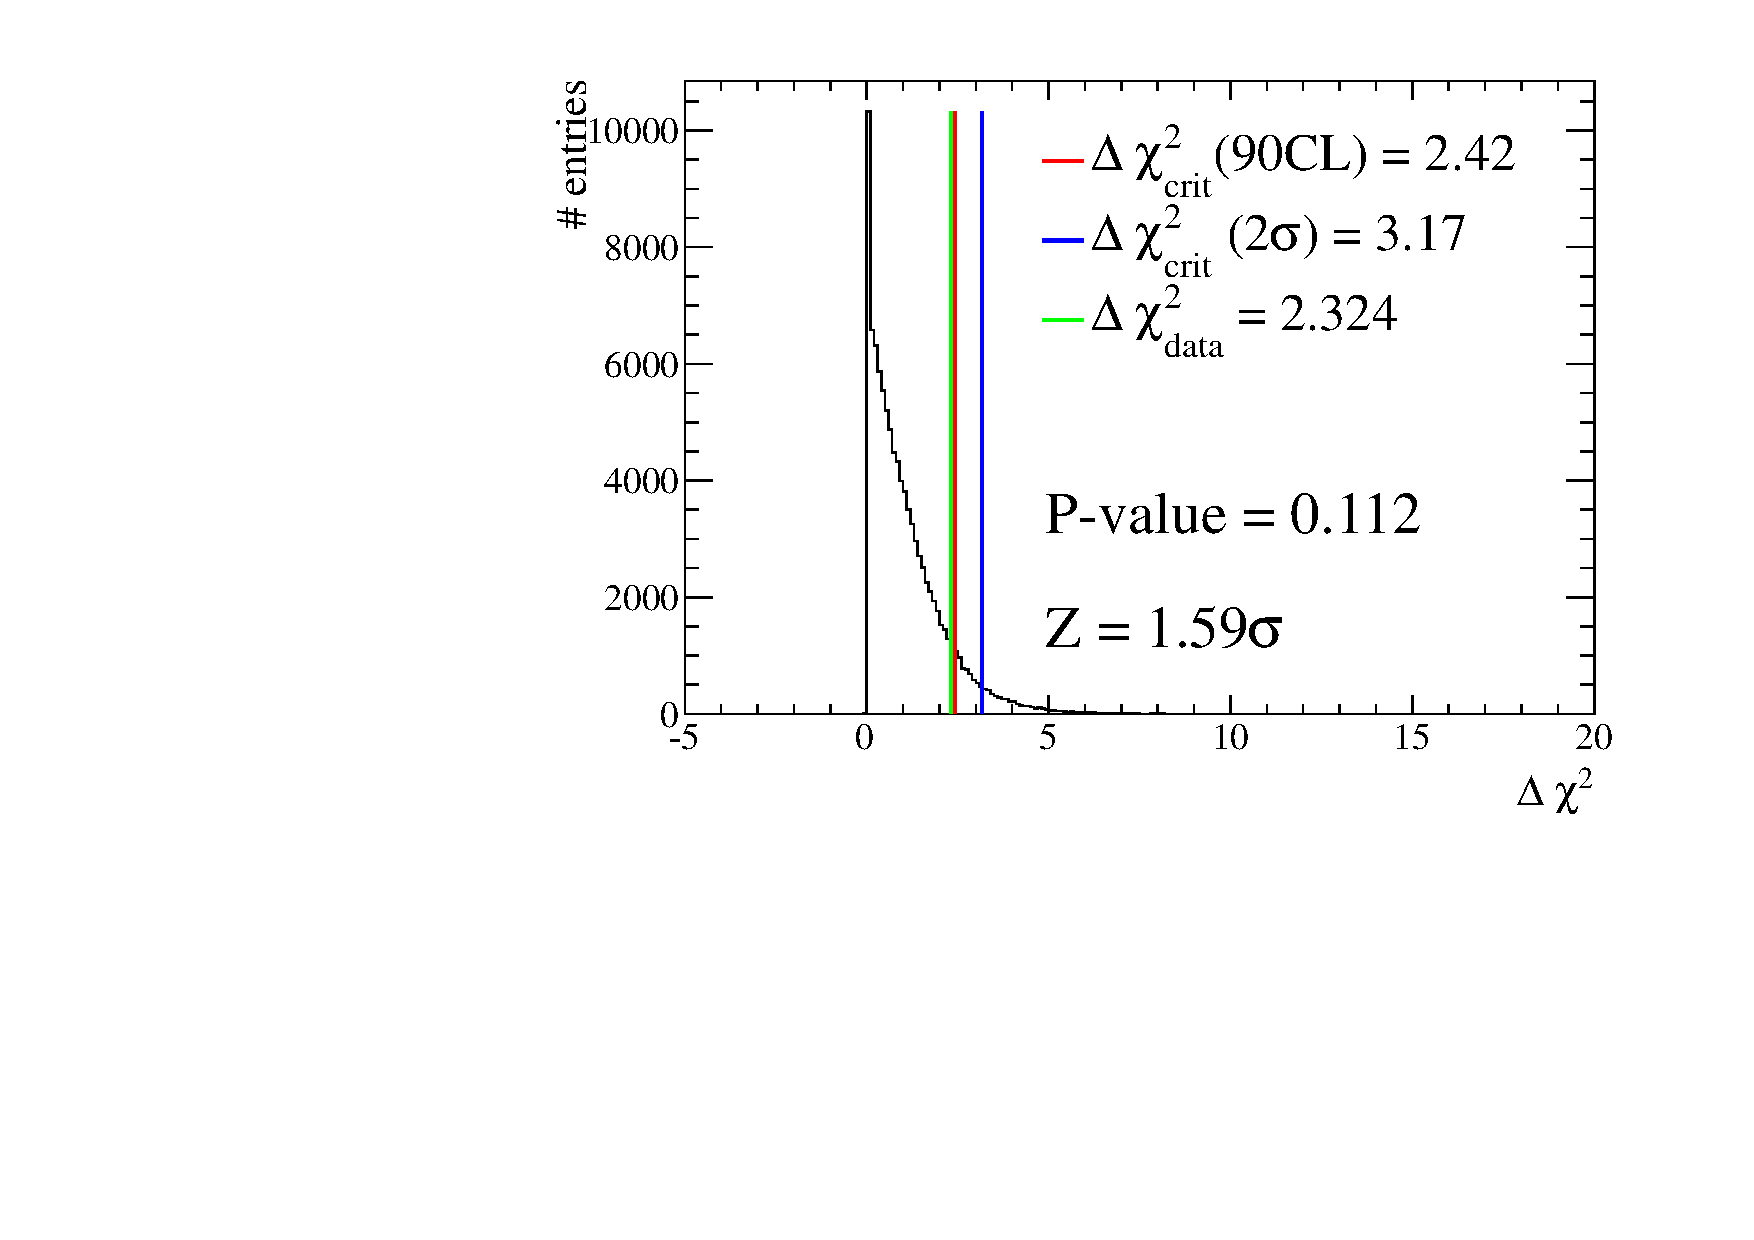
\includegraphics[width=0.49\textwidth]{./joint_plots/coverage_fc/posterior_predictive/Asimov_A/Asimov_A_deltachisq_glob_deltacp_0_normal.pdf}
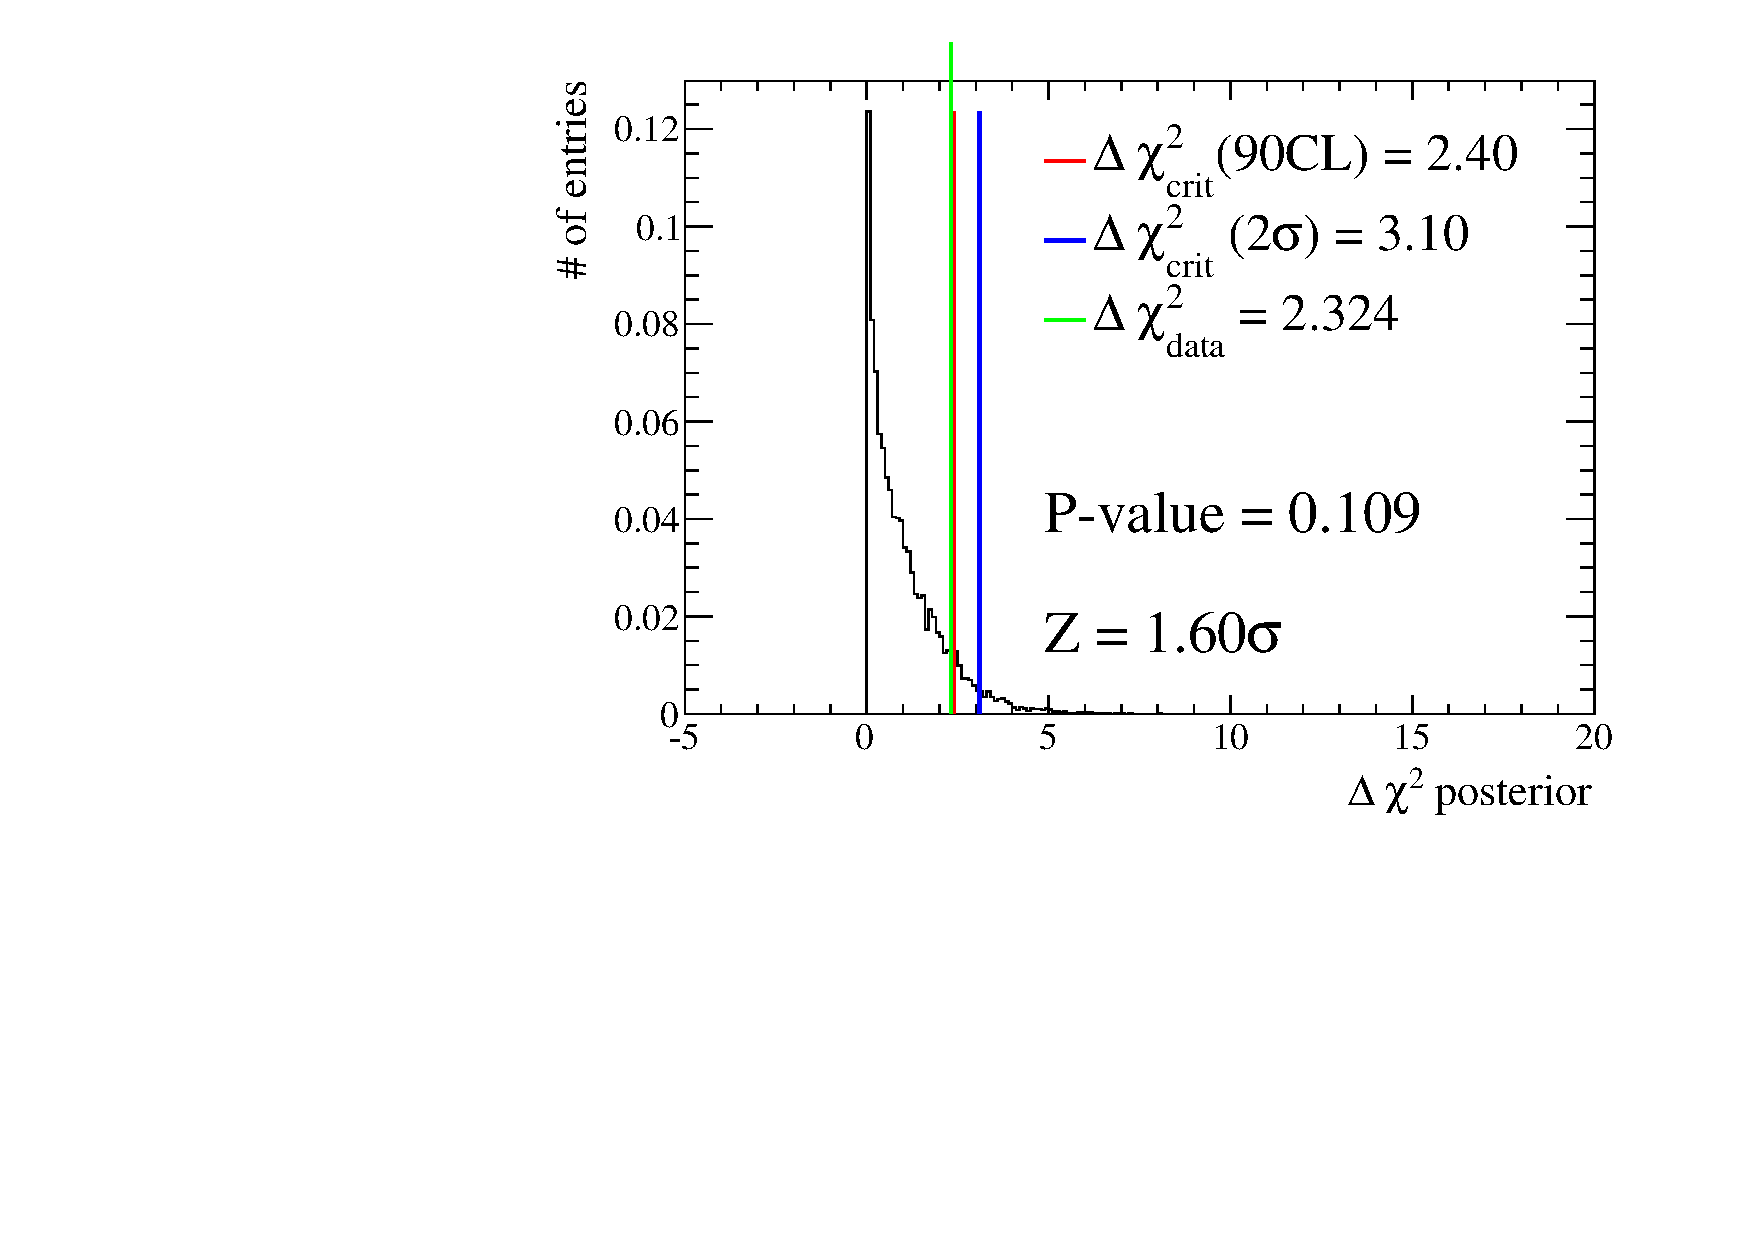
\includegraphics[width=0.49\textwidth]{./joint_plots/coverage_fc/posterior_predictive/Asimov_A/Asimov_A_deltachisq_posterior_deltacp_0_normal.pdf} \\
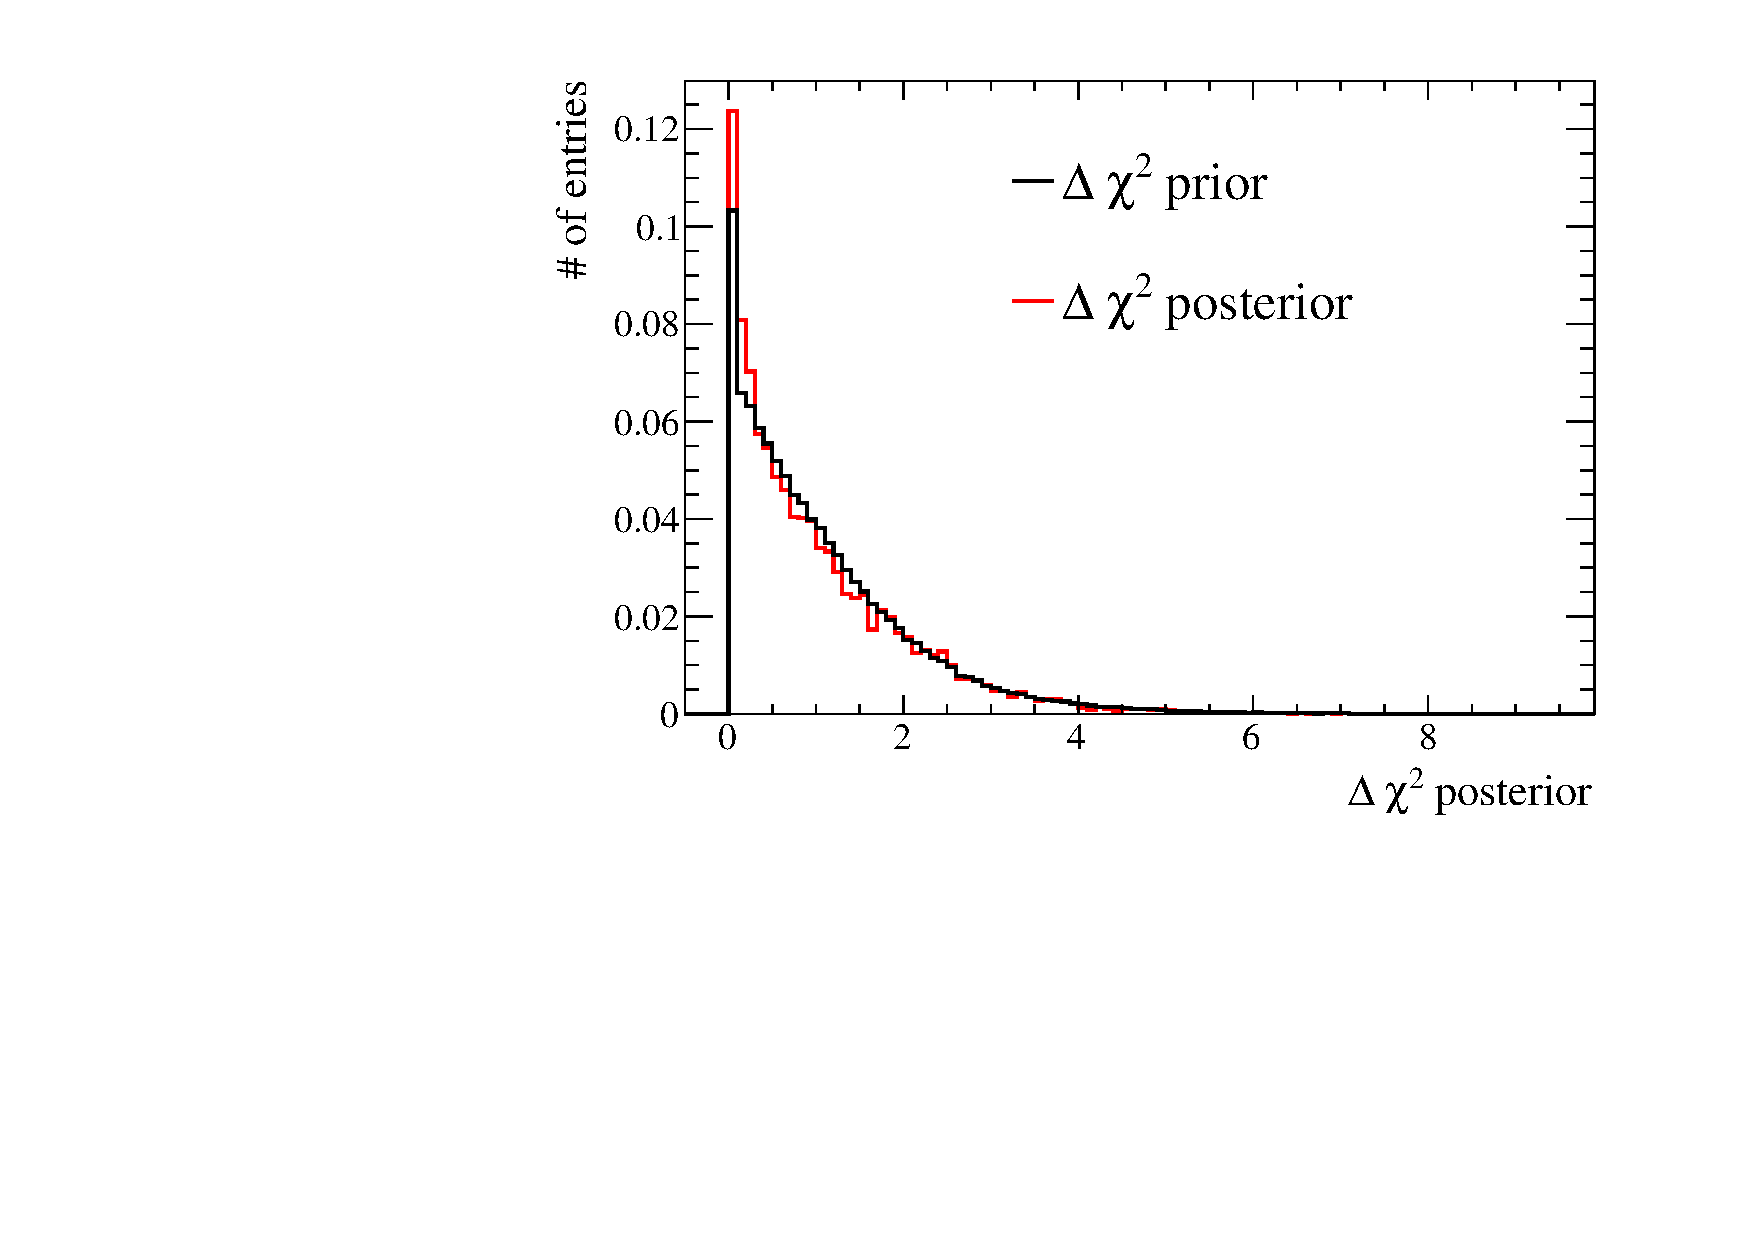
\includegraphics[width=0.49\textwidth]{./joint_plots/coverage_fc/posterior_predictive/Asimov_A/Asimov_A_deltachisq_comparison_deltacp_0_normal.pdf}
\caption {
$\Delta \chi^2$ distributions with prior (left) and posterior (right) predictive methods.
In the bottom plot the comparison between the two distributions normalized to 1 is shown.
Fake data sets are generated with $\delta_{CP} = 0$ and normal hierarchy.
The Asimov data A is used both to generate the weights of the fake data sets as well as to estimate the p-value.
50k fake data sets are used.
Since the posterior predictive distribution is weighted, the effective number of entries is lower with respect 
to the prior predictive case. 
}
\label{fig:post_Asimov_A_dcp_0_nh}
\end{figure*}


In \cref{tab:critval_posterior_Asimov_A} and~\ref{tab:critval_posterior_Asimov_B} the critical values 
calculated with the prior and posterior predictive methods for different true values of $\delta_{CP}$ and
mass hierarchy and both Asimov data set A and B.
Since the fake data set reweighting decreases the effective number of fake data sets, 
more than 10k toys experiments (the number used in the standard analysis) are needed.
For this reason at least 50k toy experiments were performed. 
The errors were calculated assuming the critical values to follow the weighted binomial distribution as explained in 
appendix \ref{app:p_value_stat_error}. 
It was also checked that 50k toy experiments are enough, since adding other 50k 
does not change much the critical values, even the ones at $2\sigma$ CL, which affect the tail of the $\Delta \chi^2$ distribution. 
The result was that the critical values for prior and posterior predictive methods are very similar
and the confidence intervals will not change much by adopting either of the two methods.

\begin{table}
\center
\begin{tabular}{| c | c | c |}
\hline
{\bf CL} 				& {\bf Prior} &{\bf Posterior}  \\
\hline
\hline
\multicolumn{3}{| c | }{$\delta^{true}_{CP} = 0$, $MH^{true} = \text{normal}$}  \\
\hline
$1\sigma$				& 1.306 		& $1.247 ^{+0.017}_{-0.017}$	\\ \hline	
90\%					& 2.424 		& $2.402 ^{+0.022}_{-0.027}$	\\ \hline	
$2\sigma$				& 3.174		& $3.102 ^{+0.057}_{-0.040}$	\\ \hline	
\hline
\hline
\multicolumn{3}{| c | }{$\delta^{true}_{CP} = 0$, $MH^{true} = \text{inverted}$}  \\
\hline
$1\sigma$				& 1.287  		& $1.278 ^{+0.021}_{-0.014}$	\\ \hline	
90\%					& 2.473  		& $2.556 ^{+0.039}_{-0.050}$	\\ \hline	
$2\sigma$				& 3.241 		& $3.355 ^{+0.071}_{-0.038}$	\\ \hline	
\hline
\multicolumn{3}{| c | }{$\delta^{true}_{CP} = -1.351$, $MH^{true} = \text{inverted}$}  \\
\hline
$1\sigma$				& 1.101  		& $ 1.065^{+0.015}_{-0.017}$	\\ \hline	
90\%					& 2.225 		& $ 2.071^{+0.039}_{-0.051}$	\\ \hline	
$2\sigma$				& 3.145		& $ 2.919^{+0.069}_{-0.062}$	\\ \hline	
\hline
\end{tabular}
\caption{
The critical values of $\Delta \chi^2$ computed with Feldman-Cousins
for both prior and posterior predictive method are shown.
50k toy experiments were used for the true point 
$\delta_{CP} = -1.351$ and inverted hierarchy
and 100k toy experiments were used for the true points
$\delta_{CP} = 0$ and normal hierarchy
and
$\delta_{CP} = 0$ and inverted hierarchy.
The weights of the fake data sets were generated with the Asimov data set A.
}             
\label{tab:critval_posterior_Asimov_A}                                                                                                                                                                             
\end{table}


\begin{table}
\center
\begin{tabular}{| c | c | c |}
\hline
{\bf CL} 				& {\bf Prior} &{\bf Posterior}  \\
\hline
\hline
\multicolumn{3}{| c | }{$\delta^{true}_{CP} = 0$, $MH^{true} = \text{normal}$}  \\
\hline
$1\sigma$				&1.306  		& $1.244 ^{+0.012}_{-0.014}$	\\ \hline	
90\%					&2.424  		& $2.448 ^{+0.018}_{-0.024}$	\\ \hline	
$2\sigma$				&3.174 		& $3.235 ^{+0.052}_{-0.037}$	\\ \hline	
\hline
\hline
\multicolumn{3}{| c | }{$\delta^{true}_{CP} = 0$, $MH^{true} = \text{inverted}$}  \\
\hline
$1\sigma$				&1.287  		& $1.231 ^{+0.013}_{-0.014}$	\\ \hline	
90\%					&2.473  		& $2.416 ^{+0.022}_{-0.025}$	\\ \hline	
$2\sigma$				&3.241 		& $3.174 ^{+0.039}_{-0.038}$	\\ \hline	
\hline
\hline
\multicolumn{3}{| c | }{$\delta^{true}_{CP} = -1.351$, $MH^{true} = \text{inverted}$}  \\
\hline
$1\sigma$				&1.101  		& $1.079 ^{+0.014}_{-0.015}$	\\ \hline	
90\%					& 2.225 		& $2.231 ^{+0.039}_{-0.035}$	\\ \hline	
$2\sigma$				& 3.145		& $3.239 ^{+0.101}_{-0.069}$	\\ \hline	
\end{tabular}
\caption{
The critical values of $\Delta \chi^2$ computed with Feldman-Cousins
for both prior and posterior predictive method are shown.
50k toy experiments were used for the true point 
$\delta_{CP} = -1.351$ and inverted hierarchy
and 100k toy experiments were used for the true points
$\delta_{CP} = 0$ and normal hierarchy
and
$\delta_{CP} = 0$ and inverted hierarchy.
The weights of the fake data sets were generated with the Asimov data set B.
}             
\label{tab:critval_posterior_Asimov_B}                                                                                                                                                                             
\end{table}

The most critical oscillation parameter for the combined measurement of  $\delta_{CP}$ and mass hierarchy
is $\sin^2 \theta_{23}$ since it affects the normalization of the $e$-like samples. % and its prior is flat.
A test was done in order to check the impact of different values of $\sin^2 \theta_{23}$ on the measurement.
Critical values were computed by generating the fake data sets without flat priors.
The only parameters that were randomly extracted in the toy generation were the solars and $\theta_{13}$,
i.e. the ones well constrained by external measurements. 
$\Delta m^2_{32}$ is kept fixed to $2.5 \times 10^{-3}~\text{eV}^2$ and 
$\sin^2 \theta_{23}$ is fixed to three different values, respectively 0.35, 0.5 or 0.65.
Since the only randomized oscillation parameters are the ones constrained by external measurements, 
there is no need to perform many toy experiments this time.
In \cref{tab:critval_posterior_sinsqth23_Asimov_A} and \cref{tab:critval_posterior_sinsqth23_Asimov_B}
the computed critical values are shown. 
Prior and posterior predictive methods give similar critical values for Asimov data set A (the most similar to our data)
and slightly different values only for the Asimov data set B
and $\sin^2 \theta_{23} = 0.35$ and $0.65$, the most extreme cases.
%$\Delta \chi^2 \sim 0.1\text{-}0.2$ in the worst case.
%If $\sin^2 \theta_{23} = 0.65$ the posterior critical values are smaller 

\begin{table}
\center
\begin{tabular}{| c | c | c |}
\hline
{\bf CL} 				& {\bf Prior} &{\bf Posterior}  \\
\hline
\hline
\multicolumn{3}{| c | }{$\sin^2 \theta_{23} = 0.35$}  \\
\hline
$1\sigma$				&1.343  		& $1.337 ^{+0.047}_{-0.041}$	\\ \hline	
90\%					&2.597  		& $2.553 ^{+0.093}_{-0.073}$	\\ \hline	
$2\sigma$				&3.423 		& $3.411 ^{+0.149}_{-0.144}$	\\ \hline	
\hline
\hline
\multicolumn{3}{| c | }{$\sin^2 \theta_{23} = 0.5$}  \\
\hline
$1\sigma$				&1.264  		& $1.229 ^{+0.026}_{-0.030}$	\\ \hline	
90\%					&2.462 		& $2.431 ^{+0.041}_{-0.037}$	\\ \hline	
$2\sigma$				&3.278 		& $3.237 ^{+0.044}_{-0.052}$	\\ \hline	
\hline
\hline
\multicolumn{3}{| c | }{$\sin^2 \theta_{23} = 0.65$}  \\
\hline
$1\sigma$				&1.244  	 	& $1.210 ^{+0.028}_{-0.022}$	\\ \hline	
90\%					&2.238  		& $2.170 ^{+0.069}_{-0.060}$	\\ \hline	
$2\sigma$				&2.816 		& $2.796 ^{+0.073}_{-0.105}$	\\ \hline	
\end{tabular}
\caption{
The critical values of $\Delta \chi^2$ computed with Feldman-Cousins
for both prior and posterior predictive are shown.
5.6k toy experiments were performed. 
The weights of the fake data sets were generated with the Asimov data set A.
The true oscillation parameters are $\delta^{true}_{CP} = 0$ and $MH^{true} = \text{normal}$
for all the toy experiments.
}             
\label{tab:critval_posterior_sinsqth23_Asimov_A}                                                                                                                                                                             
\end{table}

\begin{table}
\center
\begin{tabular}{| c | c | c |}
\hline
{\bf CL} 				& {\bf Prior} &{\bf Posterior}  \\
\hline
\hline
\multicolumn{3}{| c | }{$\sin^2 \theta_{23} = 0.35$}  \\
\hline
$1\sigma$				&1.343  		& $1.375 ^{+0.028}_{-0.037}$	\\ \hline	
90\%					&2.597  		& $2.685 ^{+0.087}_{-0.052}$	\\ \hline	
$2\sigma$				&3.423 		& $3.580 ^{+0.225}_{-0.116}$	\\ \hline	
\hline
\hline
\multicolumn{3}{| c | }{$\sin^2 \theta_{23} = 0.5$}  \\
\hline
$1\sigma$				&1.264  		& $1.239 ^{+0.026}_{-0.032}$	\\ \hline	
90\%					&2.462 		& $2.453 ^{+0.068}_{-0.035}$	\\ \hline	
$2\sigma$				&3.278 		& $3.269 ^{+0.065}_{-0.041}$	\\ \hline	
\hline
\hline
\multicolumn{3}{| c | }{$\sin^2 \theta_{23} = 0.65$}  \\
\hline
$1\sigma$				&1.244	  	& $1.177 ^{+0.027}_{-0.038}$	\\ \hline	
90\%					&2.238  		& $2.082 ^{+0.028}_{-0.043}$	\\ \hline	
$2\sigma$				&2.816 		& $2.647 ^{+0.060}_{-0.064}$	\\ \hline	
\end{tabular}
\caption{
The critical values of $\Delta \chi^2$ computed with Feldman-Cousins
for both prior and posterior predictive are shown.
5.6k toy experiments were performed. 
The weights of the fake data weights were generated with the Asimov data set B.
The true oscillation parameters are $\delta^{true}_{CP} = 0$ and $MH^{true} = \text{normal}$
for all the toy experiments.
}             
\label{tab:critval_posterior_sinsqth23_Asimov_B}                                                                                                                                                                             
\end{table}

Since the prior and posterior predictive methods gives very similar results
the choice of the priors done for the analysis is safe and no bias is expected.
The prior predictive method will be used in order to compute the confidence 
intervals with correct coverage and to estimate the significance to $\delta_{CP}=0,\pi$.
The prior predictive method will be used also for the future statistical updates.


%
% Validation minimization algorithm
%

\subsection{Validation of the minimization algorithm}
\label{sec:minim_algorithm}

As explained in \cref{sec:cl}, the best-fit parameters are found by setting up 
a grid of points of the parameters of interest and calculating the $\Delta \chi^2$ for each of them.
The grid is fine enough in order to have a very small variation of the $\Delta \chi^2$ distribution
as a function of the parameter of interest.
The best-fit point can be found by computing the entire $\chi^2$ distribution and 
looking for the lowest $\chi^2$ value.
However since the Feldman-Cousins implies a large number of toy experiments and fits for several points of $\delta_{CP}$,
this can be very CPU time consuming.
For this reason a minimization algorithm has been developed.
Similar to MINUIT \cite{Minuit}, this algorithm uses the descent gradient:
at each point of the parameter of interests it calculates the $\chi^2$ in the adjacent points along all the
possible directions (depending on the number of dimensions) and move toward the lower one,
until it stops in a minimum.
It is worth to note the MINUIT cannot be used because the grid of points of the free parameters is discrete,
while it needs to work in a continuous space.

However the descent gradient algorithm is strongly affected by the presence of local minima and depends on the 
point of the free parameters from where the fit starts.
In order to avoid this problem the fit is performed 4 times starting from 4 different starting points: $-\pi$, $-\pi/2$, $+\pi/2$ and $+\pi$.
The method has been tested by performing $10k$ toys for normal hierarchy and $4k$ toys for inverted hierarchy for the
true points $\delta_{CP} = -\pi/2, 0, +\pi/2, +\pi$.
For all the tests the number of times where the fit stopped in a local minimum is $\leq 1/10000$. 
Similar numbers have been found for inverted hierarchy.
For all the critical values the minimization algorithm is used helping to reduce the CPU time of about 30\% - 50\%,
depending on the toy experiment.


\clearpage

